% LaTeX 2e Document.
% 
% $Id: user_man.tex,v 1.12 2006/04/19 10:27:25 vdmtools Exp $
% 

%%%%%%%%%%%%%%%%%%%%%%%%%%%%%%%%%%%%%%%%
% PDF compatibility code. 
\makeatletter
\newif\ifpdflatex@
\ifx\pdftexversion\@undefined
\pdflatex@false
%\message{Not using pdf}
\else
\pdflatex@true
%\message{Using pdf}
\fi

\newcommand{\latexorpdf}[2]{
  \ifpdflatex@ #2
  \else #1
  \fi
}

\newcommand{\pformat}{a4paper}

\makeatother
%%%%%%%%%%%%%%%%%%%%%%%%%%%%%%%%%%%%%%%%

\latexorpdf{
\documentclass[\pformat,12pt]{jarticle}
}{
\documentclass[\pformat,pdftex,12pt]{article}
}

\usepackage[dvipdfmx]{graphicx, color}
\usepackage[dvipdfmx,bookmarks=true,bookmarksnumbered=true,colorlinks,plainpages=true]{hyperref}
\usepackage{alltt}
\usepackage{makeidx}
\usepackage{ifthen}
\usepackage{verbatim}
\usepackage{cite}

\usepackage{toolbox}
\usepackage{vdmsl-2e}

\usepackage{vpp}

\usepackage{ascmac}

\graphicspath{{figures/}}
\def\seename{$\Rightarrow$}

\ifnum 42146=\euc"A4A2 \AtBeginDvi{\special{pdf:tounicode EUC-UCS2}}\else
\AtBeginDvi{\special{pdf:tounicode 90ms-RKSJ-UCS2}}\fi

\makeindex

\def\vdmsl{{\small VDM-SL}}
\def\vdmpp{{\small VDM}++}
\newcommand{\vdmslpp}{VDM++}
\newcommand{\vdmslppEm}{VDM++}
\newcommand{\ToolboxName}{VDM++ Toolbox}
\newcommand{\Toolbox}{Toolbox}
\newcommand{\toolbox}{Toolbox}
\newcommand{\vdmde}{vppde}
\newcommand{\vdmgde}{vppgde}
\newcommand{\vdmhome}{vpphome}
%\newcommand{\vdmdeNineteen}{vppde} % not in use
\newcommand{\vdmdeNineteenEl}{vppde.el}
\DeclareRobustCommand{\VdmSlPp}{VDM++-\VdmSl}
\newcommand{\vdmext}{vpp}
\newcommand{\vdmModView}{\guicmd{VDMビュー}}

\newcommand{\vdmtoolsver}{v8.3.2}

\newcommand{\cg}{\vdmslpp\ to C++ Code Generator}

\newcommand{\subsubsubsection}[1]{\paragraph{#1}\mbox{}\\}

%%%%%%%%%%%%%%%%%%%%%%%%%%%%%%%%%%%% translated comment by teramoto
% 基本的にVDMSL/のifdefの使用はLaTeXのifthenelseの使用に置き換えられている。
% このため、二つのLaTeX Boolean値VDMSL、VDMppが定義されている(pが小文字なのは環境変数
% と区別するためである)使用方法は以下のとおり
%   \ifthenelse{\boolean{VDMsl}}{vdmsl-text}{vdmpp-text} ←本文ではほとんどこれが使われている
%   \ifthenelse{\boolean{VDMsl}}{vdmsl-text}{}
%   \ifthenelse{\boolean{VDMpp}}{vdmpp-text}{}
% ifdefに対し\ifthenelseを使うことの利点は、地の文中に問題を招く空行なしでVDM-SL やVDM++に特有の部分を
% 区別しつつ、埋め込むことができるところにある。
%%%%%%%%%%%%%%%%%%%%%%%%%%%%%%%%%%%% translated comment by teramoto end
% The values are initialised such that exactly one of the values is true
% and the other is false.  This should hopefully avoid strange behaviour
% due to possible preprocessing errors.  The default case is VDM-SL.
\newboolean{VDMsl}
%\setboolean{VDMsl}{true}
\newboolean{VDMpp}
%\setboolean{VDMpp}{false}
\newboolean{VDMrt}
\setboolean{VDMsl}{false}
\setboolean{VDMpp}{true}
\setboolean{VDMrt}{false}

% This macro can be used in `description' lists where
% the item given to `meti' is put on its own line,
% thereby giving proper (nicer) identation to the
% explanation.
\newcommand{\meti}[1]{\item[#1]\mbox{}\\}

\newcommand{\Index}[1]{#1\index{#1}}

\newcommand{\Lit}[1]{`#1\Quote}
\newcommand{\Rule}[2]{
  \begin{quote}\begin{tabbing}
    #1\ \ \= = \ \ \= #2  ; %    Adds production rule to index
  \end{tabbing}\end{quote}
  }
\newcommand{\SeqPt}[1]{\{\ #1\ \}}
\newcommand{\lfeed}{\\ \> \>}
\newcommand{\OptPt}[1]{[\ #1\ ]}
\newcommand{\dsepl}{\ $|$\ }
\newcommand{\dsep}{\\ \> $|$ \>}
\newcommand{\Lop}[1]{\Lit{\kw{#1}}}
\newcommand{\Sig}[1]{\Lit{{\tt #1}}}
\newcommand{\blankline}{\vspace{\baselineskip}}
\newcommand{\Brack}[1]{(\ #1\ )}
\newcommand{\nmk}{\footnotemark}
\newcommand{\ntext}[1]{\footnotetext{{\bf Note: } #1}}

%\usepackage[]{color}
\usepackage{longtable}
\usepackage{float}
\definecolor{covered}{rgb}{0,0,0}     %black
\definecolor{not_covered}{gray}{0.5}  %gray

%\restylefloat{figure}
\setcounter{topnumber}{3}
\def\topfraction{1.0}
\setcounter{bottomnumber}{3}
\def\bottomfraction{1.0}
\setcounter{totalnumber}{3}
\def\textfraction{.1}


\parindent0mm

\newlength{\keywwidth}

\newcommand{\xfigpicture}[4]{
\begin{figure}[hbt]
\setlength{\unitlength}{1mm}
\begin{center}
\mbox{
\begin{picture}(#1,#2)
\put(0,0){\special{psfile=#3 hscale=70 vscale=55}}
\end{picture} }
\end{center}
\caption{#4}
\end{figure}
}

%\newcommand{\qq}{\marginpar{\bf ???}}
\newcommand{\aaa}{\tt }
\newcommand{\cmd}{\tt }
\newcommand{\guicmd}[1]{{\gt #1}}
\newcommand{\keyw}[1]{{\sf #1}}
%\newcommand{\id}[1]{%
%  \settowidth{\keywwidth}{\tt #1}%
%  \protect\makebox[\keywwidth][l]{{\it #1}}}
%\nolinenumbering

\begin{document}
\vdmtoolsmanualscsk{VDMTools ユーザマニュアル (\vdmslpp)}
       {\ifthenelse{\boolean{VDMrt}}{2.0 beta}{2.0}}

\section{はじめに} \label{introduction}

%This manual presents an introduction to the \vdmslpp\ \Toolbox.


\VDMTools\ は、コンピュータシステムの精巧なモデルを開発・分析するツールである。
システム開発の早期に導入すれば、これらのモデルはシステム仕様として、
あるいはユーザの要求の網羅性や整合性のチェックを助けるものとして役立つ。
モデルは、ISO VDM-SL 標準言語~\cite{ISOVDM96}\index{VDMひょうじゅん@VDM標準}、
あるいは、オブジェクト指向形式仕様言語VDM++\cite{LangManPP-SCSK}\cite{Fitzgerald&05}によって表現される。
本マニュアルでは、実装に先立ち、 \vdmslpp\ で表現されたモデルの自動チェックと検証を行うためのツールである
 \vdmslpp\ ツールボックスについて記述する。
その範囲は、従来からの構文と型のチェックツールから、必要に応じてモデルを実行し、
実行中には自動的に整合性チェックを行う強力なインタープリタに及ぶ。
実行機能は、分析・設計の早期からテスト技術の利用を可能にするとともに、
確立されているソフトウェアエンジニアリングの実践に即した全体的なテストの実行を可能にする。
そのうえ、このインタープリタでは、ブレイクポイントの設定、文のステップ実行、
表現の評価、コールスタックの調査、スコープにおける変数の値のチェックなど、
モデルのインタラクティブなデバッグが可能である。

本ドキュメントには \vdmslpp\ ツールボックス(この文書では \Toolbox\ と呼ぶ)の紹介とリファレンスマニュアルを記載する。
\vdmslpp\ 言語には別に言語マニュアルがある。
\ifthenelse{\boolean{VDMsl}}{\cite{LangMan-SCSK}}{\cite{LangManPP-SCSK}}.
このマニュアルでは、{\em 仕様\/}という言葉は目的を問わず本言語で構成されたすべてのモデルを指すものとして使う

\subsection*{VDM入力フォーマット}\index{インプット!フォーマット}


\Toolbox\ はMS Wordまたは \LaTeX\ の文書に埋め込まれた \vdmslpp\ の仕様をサポートしているので、
仕様を抜き出したファイルを別途作ることなく、仕様の分析を行うことができる。
システムのモデルとその文書を統合して扱う方法として、これらの書式を使用することを推奨する。
モデルの記述と文書を統合して扱うことで、
最新版の仕様と文書化されている仕様の不整合を避けることができる。
もちろん、Word や \LaTeX\ を使用しなくてもよく、好みのテキストエディタを使って、
シンプルなテキストファイルの仕様を書くことも出来る。

仕様は日本語を使って記述することができ、\Toolbox\ を使って解析することができる。
\Toolbox\ は複数の文字コードを入力文書としてサポートしている。
付録~\ref{sec:generic}\index{インプット!いっぱん@一般}
で \Toolbox\ への文字コードの設定方法を説明している。

MS Wordを使用して\vdmslpp\ の仕様を作成する場合は、仕様を記述した文書を
{\em Rich Text Format\/}~(RTF)フォーマットで保存しなくてはならない。
\Toolbox\ の配布パッケージには、このフォーマットでのサンプルファイルが含まれる。
このマニュアルでは、\Toolbox\ の配布パッケージに含まれるそれらのファイルを使った例を参照している。
例題のファイルで、``{\tt .rtf}''が拡張子がついていれば、リッチテキストフォーマット(RTF)のファイル
であることがわかる。

このマニュアルでは、\Toolbox\ の機能の紹介を Word の RTF を前提として行う。
\LaTeX\ で仕様を作成するのであれば、
付録~\ref{sec:latexANDvdm}に書かれているフォーマットとスタイルを使って
\LaTeX\ のコマンドにVDM仕様を埋め込む方法を参照してほしい。
\Toolbox\ にはこのフォーマットでもサンプルファイルが入っているが、
拡張子は``{\tt .rtf}''ではなく``{\tt .\vdmext}''である。そのため、例が{\tt sort.rtf}というファイルを
参照していた場合、代わりに{\tt sort.\vdmext}というファイルを使わなくてはいけない。
ディレクトリ構造の参照はこのマニュアルを通じて以下のような形式で示される。

{\tt examples/sort.vdm} (スラッシュ区切り)  
Windowsでは\verb+examples\sort.vdm+ (英語ではバックスラッシュ区切り).と同じである。

シンプルなテキストファイルとして仕様を記述した場合、説明文を仕様に
組み込む唯一の方法は、言語マニュアルに記載されている
\vdmslpp\ コメント構文を用いることだ。このフォーマットについては通常拡張子
``{\tt .\vdmext}''でファイルが用意されている。

\subsection*{このマニュアルの使い方}


このマニュアルは3つの部分に分かれる。セクション~\ref{sec:overview}と~\ref{sec:guidedtour} は
\Toolbox\ のさまざまなツールの概略とGUIを利用した\Toolbox\ のチュートリアルを提供する。
マニュアルのこの部分を実際に試してみる前に、\Toolbox\ がインストールされていなくては
ならない(付録~\ref{sec:set_env}参照)。\Toolbox\ のインストールについてはこの文書に記述される
\ifthenelse{\boolean{VDMsl}}{\cite{InstallMan-SCSK}}{\cite{InstallPPMan-SCSK}} 。
セクション~\ref{sec:guidedtour}を読み進むにつれ、さまざまなツールや制御コマンドを利用できることが
わかるだろう。

第2のパート~(セクション~\ref{sec:ref})は、\Toolbox\ のシステム的なすべての機能を
カバーするリファレンスガイドである。
3つの利用可能なインターフェースすべて(コマンドラインインターフェース、Emacsインターフェース、
GUI)について、それぞれの機能を記述してある。

このマニュアルの第3のパートは一連のトピックスについての付録で構成されている。
付録~\ref{sec:vdmlinks}はVDMの情報源について記載されているが、これにはインターネットのサイト、
プロジェクトの記述、技術論文や参考文献が含まれている。付録\ref{sec:latexANDvdm}では\LaTeX\ の文書
でどのようにテキストと仕様をマージするかを説明している。

付録~\ref{sec:set_env}では環境を\Toolbox\ 向けにどう設定するかが記述されている。
付録~\ref{getting-started}ではEmacsインターフェースについて。
付録~\ref{sec:testscript}にはSort仕様(このマニュアルで実行可能な例として使われている)
のシステムテストに使うテストスクリプトがいくつか含まれている。\ifthenelse{\boolean{VDMsl}}{そして}{}
付録~\ref{sec:trouble} では\Toolbox\ を使っていると見られるMicrosoft Wordにおいての一般的な問題について、
考えうる解決策をいくつか提供している。\ifthenelse{\boolean{VDMsl}}{}
{さらに、付録~\ref{sec:priorityfile}では、インタープリタで使うファイルの優先順位の定義用の
フォーマットが記述されている。}

\newpage

\section{\protect\VDMTools\ の概略}\label{sec:overview}


\vdmslpp\ 仕様は、システムの特性を厳密に記述することを目的としたドキュメントである。
この仕様は、セクション~\ref{introduction}で記述されている入力フォーマットで書かれた複数のファイルに
分かれていることもある。図~\ref{fig:toolbox}は\Toolbox\ の機能の概要とその付属的な機能を示したものである。
ツールについては下記に記述する。

\begin{figure}
\begin{center}
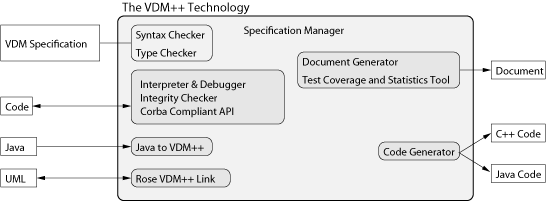
\includegraphics[width=10cm]{vdmtools_pp.png}
\caption{\protect\VDMTools\ の概略}
\label{fig:toolbox}
\end{center}
\end{figure}

\begin{description}
  

\item[マネージャー] 仕様に定義されている\ifthenelse{\boolean{VDMsl}}{モジュール}{クラス}
の状態を常に保持する。仕様は、複数のファイルで構成されていることもあり、それらすべての状態を保持する。

\item[構文チェック機能] \vdmslpp\ 言語の定義に照らして、\vdmslpp\ の仕様の構文が正しいか
どうかチェックする。構文が受け入れられれば、\Toolbox\ 内の他ツールの利用が可能となる。

\item[型チェック機能] 強力な型推論メカニズムを持ち、値や演算子の誤用を特定する。
またランタイムエラーの起こりうる箇所も示す。

\item[インタープリタとデバッガ] インタープリタは、\vdmslpp\ で実行可能な構成要素すべてを実行する。
その範囲は、集合の内包式や列の列挙式など単純な構成子から、より複雑な構成要素
(例外処理、ラムダ表現、ルーズな表現やパターンマッチング\ifthenelse{\boolean{VDMpp}}{、マルチスレッドモデルまでも}{})
にも及ぶ。仕様を実行することの利点の一つは、
テスト技術がこれらの検証に役立つということだ。開発プロセスにおいて、
仕様の小(大)部分が設計者の理解と自信を深めるのに有効である。その上、
実行可能な仕様は実行プロトタイプを形成する。

ソースレベルのデバッガは、実行可能な仕様を用いて作業をする上で、
必要不可欠な機能である。\vdmslpp\ デバッガは、ブレイクポイントの設定、ステップ実行、
スコープ内で定義された変数の値チェック、
コールスタックのチェックなど、通常のプログラミング言語向けのデバッガと同様の機能をサポートする。

\item[証明課題生成機能] 証明課題生成機能は、 \vdmslpp\ ツールボックスの型チェックの機能を
拡張するものである。仕様全体をスキャンして、内的矛盾点や整合性を侵害しうる潜在的なソースをチェックする。
データ型の不変条件、事前条件、事後条件、
列の境界や写像のドメインの違反チェックが含まれる。\emph{証明課題}は\vdmslpp\ の式で表され、
trueと評価されなければならない。もしfalseと評価されていたら、それは仕様の相当する箇所に
潜在的な問題があることを示している。

\item[テスト機能] テスト機能では{\em テストスイート\/}と呼ばれる予め用意されたテストセットを
使って、仕様の実行が可能である。テストカバレッジ情報は、テストスイートの実行中に自動的に記録され、
あとから、仕様のどの部分が頻繁に評価されているか、どの分が全くカバーされていないかなどを、
表示する。テストカバレッジ情報は、仕様がWordまたは \LaTeX\ で記述されている場合には、
ソースファイル文書に直接表示することができる。

\item[自動コード生成] Toolboxは、\vdmslpp\ の仕様から\ifthenelse{\boolean{VDMsl}}{C++}{C++とJava}の
コードを自動生成する機能をサポートしており、この機能により仕様と実装の間に一貫性を持たせることができる。
コード生成機能は\vdmslpp\ の構文の95\%\ から実行可能なコードを生成する。仕様の実行不可能な箇所向けに、
ユーザによる定義コードを含めることを可能にする機能も併せ持つ。いったん仕様がテストされれば、
コード生成機能を迅速な実装を自動的に得る手段として利用できる。C++のコード生成機能の使い方は
本ドキュメント\ifthenelse{\boolean{VDMsl}}{\cite{CGMan-SCSK}}{\cite{CGManPP-SCSK}}に記載されている。
\ そしてJavaコード生成機能の使い方は本ドキュメント\cite{CGJavaManPP-SCSK}に記載されている。

\item[動的リンク機能] 外部のコードを仕様の実行に加えることを可能にする。
この機能により、伝統的な方法で開発されたコンポーネントで構成される形式モデルを結合したり、
モデルにグラフィカルなフロントエンドを提供するといったことが可能になる。

\item[Corba対応API] \Toolbox\ はCorba対応APIを提供しており、これにより
実行中の\Toolbox\ に他のプログラムがアクセスできる。これは型チェック機能やインタープリタ、
デバッガなどの\Toolbox\ のコンポーネント外からの制御を可能にするものである。
APIを使えば、グラフィカルなフロントエンドやレガシーコードなど、どんなコードからでも\Toolbox\ 
へのアクセスが可能になる。

\item[UML リンク] UML リンク はUMLと\vdmpp\ を結びつける。
\Toolbox\ とXMIファイルを経由して、astah* ProfessionalやEnterprise Architectと
双方向のモデル共有を可能とする。
また、Rational RoseとはOLEを経由して双方向で緊密に結びつける変換機能を提供する。

ゆえに、このリンク機能はUML と\vdmpp のラウンドトリップエンジニアリングをサポートし、
形式的な記述が機能の詳細な振る舞いを記述するのに使われる一方で、
グラフィカルな記述が構造的でダイアグラムを利用したモデルの概略を提供するのに使われる。
UML リンクについてはドキュメント\cite{UMLMan-SCSK}に記述されている。

\item[Javaから\vdmpp\ への変換ツール] この機能は現存するJavaアプリケーションを
\vdmpp にリバースエンジニアリングするものである。アプリケーションの分析が\vdmpp レベルで
実行され、新たな機能が特定される。最終的に、新たな仕様がJavaから翻訳される。
Javaから\vdmpp への変換ツールの使い方は\cite{Java2VDMMan-SCSK}に記述されている。
注)現在この機能は、現行のJavaのすべての構文をサポートしていない(ジェネリクス、可変引数など)。

\end{description}

\newpage

\section{\protect\VDMTools ガイドツアー } \label{guistart}
\label{sec:guidedtour}


このセクションでは、\Toolbox\ の「ガイドツアー」を提供する。
VDMによるシステムモデリングを新たに学ぼうとするのであれば、
``{\it ソフトウェア開発のモデル化技法}''~\cite{Fitzgerald&98b}, J.フィッツジェラルド、P.G.ラルセン著、
または、``{\it VDM++によるオブジェクト指向システムの高品質設計と検証}''~\cite{Fitz-Larsen&2010J}
を最初に読むことをお勧めする。
これらのチュートリアルブックには、\Toolbox\ を使って探索可能な、
VDM仕様で書かれたさまざまな例題が掲載されている。
\cite{Fitzgerald&98b} ではISO標準のVDM-SLを使って記述されており、一方、
\cite{Fitzgerald&05} では \vdmpp\ と呼ばれる、オブジェクト指向拡張された言語を使って記述されている。
これらの一般的な概念を知っているが、
\ifthenelse{\boolean{VDMsl}}{標準的な記法に詳しくない人}{
\vdmslpp\ でオブジェクト指向向けに拡張された部分に詳しくない人}
には、\vdmslpp\ の言語リファレンスマニュアルである``{\it The  \vdmslpp\ Specification Language}''
\ifthenelse{\boolean{VDMsl}}{\cite{LangMan-SCSK}}{\cite{LangManPP-SCSK}}を一読すること
をお勧めする。

\subsection{\protect\VDMTools で取り扱う仕様の作成}\index{インプット!さくせい@作成}


\Toolbox\ を使用するためには、\vdmslpp\ の仕様を書いておく必要がある。
このセクションでは、シンプルなソートのサンプルを作成することを通じて、
MS Wordのリッチテキストフォーマットを使用した方法を記述する。\LaTeX\ 文書を
使いたい場合は、付録~\ref{sec:latexANDvdm}\footnote{プレーンテキストのみの\vdmslpp を
使用することも可能}を参照のこと。
このセクションでは、MS Wordを使用すると想定していることを覚えておいてほしい。

MS Wordを起動して、\Toolbox\ から
\ifthenelse{\boolean{VDMsl}}{{\tt \vdmhome/examples/sort/sort.rtf}ファイル}{
{\tt \vdmhome/examples/sort/MergeSort.rtf} ファイル}\footnote{\vdmhome は
\Toolbox\ のトップディレクトリ。Windows の場合、通常は、
C: \yen Program Files \yen The VDM++ Toolbox v?.?
となる} を開く。このファイルを一通り読めば、

このドキュメントが説明文と\vdmslpp 形式のモデルであることがわかるはずだ。形式の部分は
\texttt{VDM}スタイルですべて書かれている。
VDMスタイルの文書から直接元の文書に戻すのはおそらく無理だろう。通常のプリンタはVDM
のキーワードを太字のフォントで印刷する。このスタイルの外観を修正することはできるが、
スタイルの名前は変えられない。なぜなら\Toolbox\ が\texttt{VDM}スタイルで書かれた
文書の部分だけを解析するからである。

\Toolbox\ 内で使用されるスタイルの定義は\Toolbox\ の中にある{\tt VDM.dot}ファイル(Word形式)
\index{VDM.dotファイル}に記述されている。このファイルはテンプレートディレクトリ(通常は
\verb+C:\Program Files\Microsoft Office\Templates+ )にコピーすることで、
新しくドキュメントを作成した場合にテンプレートを選択すると(普通に使用していれば、
このほかにもさまざまな方法でテンプレートディレクトリにスタイル定義がコピーされる)これらのスタイルの定義が
含まれることになる。

\ifthenelse{\boolean{VDMsl}}{{\tt sort.rtf} ファイル}%
{{\tt MergeSort.rtf} ファイル}の最後を見てみよう。
クラス名MergeSortが\texttt{VDM\_TC\_TABLE}の形式で書かれているのがわかるだろう。
この使い方は後でテストカバレッジ情報の記録・表示方法についての話をするときに詳しく述べる。
この\texttt{VDM\_COV} および \texttt{VDM\_NCOV} 形式はテストカバレッジの情報と
関連付けるときにも使われる。
これらの形式についても後ほど述べる。

さらにMS Wordを使用して\Toolbox\ への入力物を作成する経験を積む場合は、
「ガイドツアー」を終えた後に\Toolbox\ 内のほかのサンプルファイルを読むことをお勧めする。

\subsection{GUIで \vdmslpp\ を始める}\index{GUI!スタート} 


\Toolbox\ は通常GUIを使う。GUIを使い始める前に、VDMのソースファイルがワーキングディレクトリ
にコピーされていなければならない。\Toolbox\ は異なる種類のソートアルゴリズムの仕様を含んでいるが、
これはテクニカルリポート\ifthenelse{\boolean{VDMsl}}{\cite{SortEx-SCSK}}{\cite{SortExpp-SCSK}}に書かれて
いるとおりである。このガイドツアーでは、このソート仕様をサンプルとして使うため、{\tt \vdmhome/examples/sort}
ディレクトリをコピーしてそこへディレクトリを移動してもらいたい。これで次からのツアーをあなたの環境で
\Toolbox\ 内のツールを直接試すことが出来るようになったはずだ。

\Toolbox\ はWindowsのスタートメニューから選択するか、Unix環境であれば{\tt
  \vdmgde}コマンド\index{vdmgdeコマンド}で起動する。
図~\ref{fig:startgui}は\Toolbox\ の起動画面である。このウィンドウを\Toolbox\ の
{\em メインウインドウ\/}と呼ぶ

\begin{figure}[tbh]
\begin{center}
\ifthenelse{\boolean{VDMsl}}{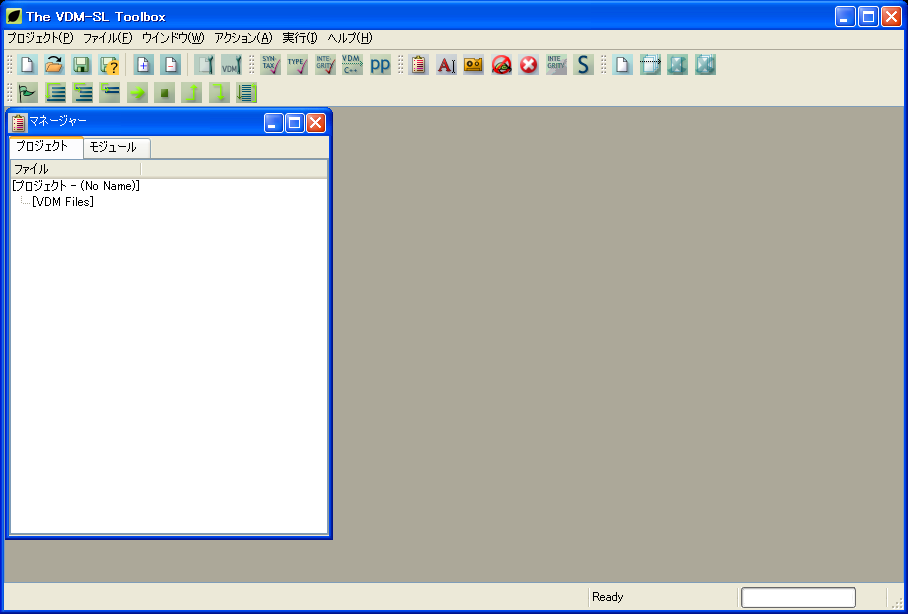
\includegraphics[width=11cm]{startgui-sl.png}}{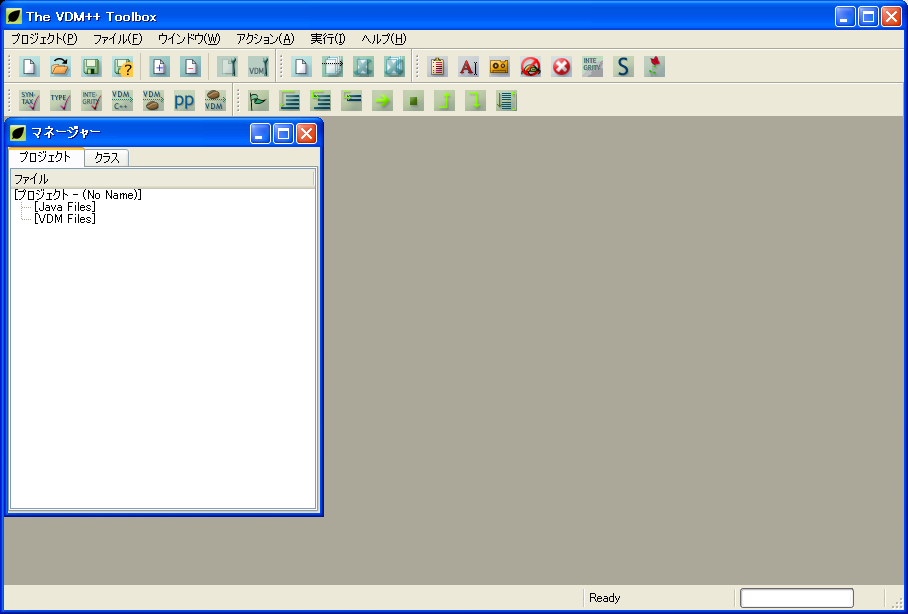
\includegraphics[width=11cm]{startgui-pp.png}}
\caption{スタートアップ画面}
\label{fig:startgui}
\end{center}
\end{figure}

\subsection{オンラインヘルプ}\index{オンラインヘルプ}
 
% %%%%% The next paragraphs should be reinserted when help window is
% %%%%% implemented -- RM
%
% At any time when you are using the \Toolbox\ you can press the ``{\tt
%   F1}'' button and a help window~(as shown in
% Figure~\ref{fig:guihelp}) will appear with
% on-line help for the 
% graphical user interface. The part of the help text that is shown at
% the top of the help window is related to the particular part of the
% \Toolbox\ window in which the cursor is placed. The help text is
% organised in a hypertext format so it is possible to follow links from
% one part of the help text to another.

% \begin{figure}[tbh]
% \begin{center}
% #ifdef VDMSL
% \resizebox{\textwidth}{!}{\includegraphics{guihelp-sl}}
% #endif VDMSL
% #ifdef 
% \resizebox{\textwidth}{!}{\includegraphics{guihelp-pp}}
% #endif 
% \caption{The Help Window\label{fig:guihelp}}
% \end{center}
% \end{figure}

% The help window can also be accessed by pressing the  
% \raisebox{-0.8mm}{
\includegraphics[width=0.03\textwidth]{help}}
% button on the \guicmd{Help} toolbar or by selecting the corresponding
% item from the \guicmd{Help} menu. 


\Toolbox\ のオンラインヘルプと一般的なインターフェースは\guicmd{ヘルプ}ツールバーや\guicmd{ヘルプ}
メニューからアクセスできる。最近では以下に示す限られたものだけが利用可能である。

\begin{description}
 \item[\guicmd{ツールについて} (\hspace{-1.8mm}
\raisebox{-0.8mm}{
\includegraphics[width=0.03\textwidth]{help.png}}):]
  \Toolbox\ のバージョン番号を表示する.
 \item[\guicmd{Qtについて}  (\hspace{-1.8mm}
\raisebox{-0.8mm}{
\includegraphics[width=0.03\textwidth]{qt.png}}):]
  Qt(\Toolbox\ のインターフェースが利用している、C++のマルチプラットフォーム
  GUIツールキット)へのリファレンス情報を表示する
% \item[\guicmd{What's This?} (\hspace{-1.8mm}
%\raisebox{-0.8mm}{
\includegraphics[width=0.03\textwidth]{whatsthis}}):]  
%  これを選択してから\Toolbox\ の一部の上でマウスの左ボタンをクリックすると、
%  その項目についての記述が表示される(現在は一部のみ実装されている)
\end{description}

\subsection{メニュー、ツールバー、サブウインドウ}

メインウインドウの上部は6つのプルダウンメニューが一列になって構成されている。

\begin{description}
\item[\guicmd{プロジェクト}:]
  プロジェクトメニューは\vdmslpp\ の仕様を構成するファイル名の集合で構成されている。
  このメニューからはプロジェクトを開く/保存する、プロジェクトの設定(ファイルの追加/削除)
  をする、新規プロジェクトの作成などができる。\Toolbox\ を終了させたり、\Toolbox\ のさまざまな
  ツールのオプションを設定する機能もここにある。(例えば型チェックのレベルを設定など)

\item[\guicmd{ファイル}:]
  ここからは仕様を訂正するためファイルエディタが起動できる。またエラーが報告されたとき、
  \Toolbox\ によって自動的に表示されるソースファイルの表示を終了させることが出来る。

\item[\guicmd{ウインドウ}:]
  メインウインドウの画面に表示されているウインドウをコントロールする。
  メニュー項目を使って、対応するウインドウの表示/非表示を行うことができる。

\item[\guicmd{実行}:]
  インタープリタのコントロール機能を提供する(セクション~\ref{interpreter}参照)。
  構文チェックや型チェック、証明課題の生成、コード生成、
JavaからVDM++へのリバースエンジニアリング、
  清書など、仕様に適用されるさまざまなアクションを提供する。

%\item[\guicmd{Help}:]
%  \Toolbox\ のオンラインヘルプや一般的なインターフェース
\end{description}

%  以下ではこのメニューの6つ\footnote{\Toolbox\ が開始された時、1番目と3番目と4番目の
%  メニューに相当するものだけが開く。残りの3つはその上にアイコン化されて表示される}あるツール
%  バーの項目について同様のアクションを提供するものを示す。
  このメニューの下には、メニューと同じ機能を提供するツールバーが配置される。
  
  メインウインドウの下部の画面は、現在のプロジェクトの状態に関する情報や
  \Toolbox\ 内のツールへのインターフェースを提供するさまざまなサブウインドウを表示する
  のに使用される。利用できるウインドウは以下のとおり:

\begin{description}
\item[\guicmd{マネージャー}]\index{マネージャー}
  現在のプロジェクトの最新状態を表示する。以下の2つのビューから構成される。

  \begin{description}
  \item[\guicmd{プロジェクトビュー}]\index{プロジェクトビュー}
  プロジェクトの内容をツリー形式で表示する。
  プロジェクトの構成ファイルとそれぞれで宣言されている\ifthenelse{\boolean{VDMsl}}{モジュール}{クラス} 
  (ファイルの構文チェックが成功したもののみ)が含まれる。
  
  \ifthenelse{\boolean{VDMsl}}{
     \item[\guicmd{モジュールビュー}]\index{モジュールビュー}
     プロジェクトに含まれる\vdmslpp\ モジュールの個々の状態を表示する。}{
     \item[\guicmd{クラスビュー}]\index{クラスビュー}
       \guicmd{VDMビュー}と\guicmd{Javaビュー}の二つがあり、プロジェクトに含まれる個々
       の\vdmslpp\ クラス・Javaファイルをそれぞれ表示する。} 
  \end{description}

\item[\guicmd{ソースウインドウ}]\index{ソースウィンドウ}
  仕様を表示する。エラーが発生した場合は、
  \guicmd{エラー一覧}でエラーを選択した場合は、その位置を表意する。

\item[\guicmd{ログウインドウ}]\index{ログウィンドウ}
  \Toolbox\ からのメッセージを表示する

% \item[\guicmd{References}] Displays the dependencies between classes,
%   that is the classes which use the selected class and the classes
%   which the selected class uses~(a class {\em uses\/} another class if it
%   has references to objects of that class, for example through its
%   instance variables or operation calls). 
\item[\guicmd{実行ウインドウ}]\index{インタープリタウィンドウ}
インタープリタとのインターフェース。

\item[\guicmd{エラー一覧}]\index{エラーリスト}
\Toolbox\ によって発見されたエラーリポート。

\item[\guicmd{証明課題ウインドウ}]\index{しょうめいかだいういんどう@証明課題ウインドウ}
  仕様から生成された証明課題を表示するウインドウ。

\item[\guicmd{識別子検索ウインドウ}]\index{しきべつしけんさくういんどう@識別子検索ウインドウ}
  仕様から識別子を検索する。定義部分のみや部分一致による検索ができる。

\item[\guicmd{UMLリンクウインドウ}]\index{UMLリンクウインドウ}
  UMLツールとの連携を操作するウインドウ。
\end{description}

\Toolbox\ の起動時には、\guicmd{マネージャー}のみが開いている。

\subsection{プロジェクトを作成する}

まず、どのファイルを分析にかけるかを\Toolbox\ に設定する必要がある。
このため、プロジェクトメニューから\guicmd{ファイルを追加}を選択するか(\guicmd{プロジェクト})
ツールバーから\raisebox{-0.4mm}{
\includegraphics[width=0.03\textwidth]{plus.png}}  
(\guicmd{ファイルを追加}) ボタンを押す\footnote{このガイドツアーでは、ツールバーのボタンを使った操作
を中心に話を進めている。メニュー項目を使っても同じ操作を行うことができる}。
すると、図~\ref{fig:addFiles}に示すようなダイアログボックスが表示される。\index{プロジェクト!ファイルついか@ファイル追加}.

\begin{figure}[tbh]
\begin{center}
\ifthenelse{\boolean{VDMsl}}{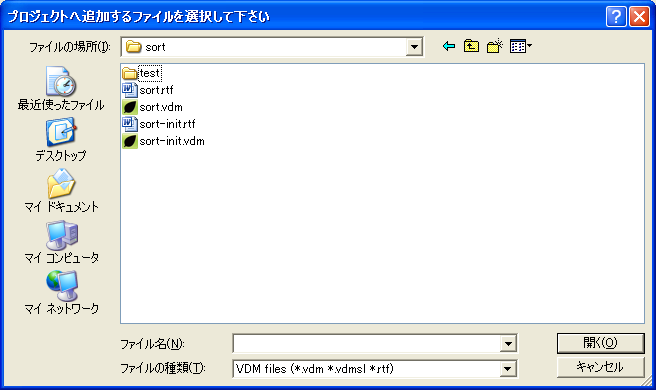
\includegraphics[width=11cm]{addFiles-sl.png}}{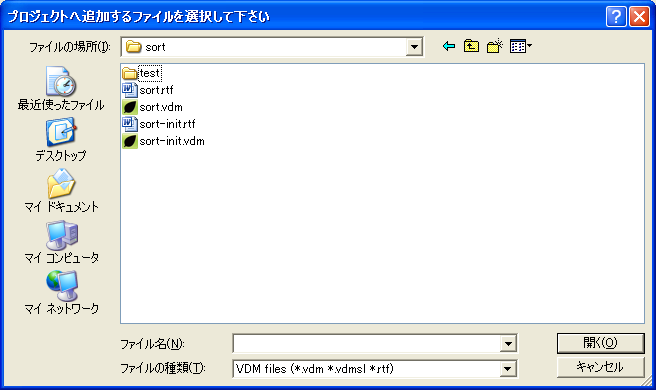
\includegraphics[width=11cm]{addFiles-sl.png}}
\caption{プロジェクトにファイルを追加する}
\label{fig:addFiles}
\end{center}
\end{figure}

\ifthenelse{\boolean{VDMsl}}
{%
sort-init.rtfファイルをダブルクリックする(またはファイルを選択のうえ``\guicmd{開く}''ボタンを押下して
プロジェクトへファイル追加)。このファイルがプロジェクトに追加されているはずだ。
{\cmd Ctrl}キー\footnote{この操作を行うためのキーはOSに依存する。Windows や Linux では{\cmd Ctrl}キー、
Mac OS X では{\cmd Command}キーとなる。}を押しながら
マウスの左ボタンをひとつずつ順番に押すことで一度に複数ファイルを選択することができ、{\cmd Shift} キーを
押しながらファイルリストの最初と最後を選択する(順番はどちらでもよい)ことで一覧のファイルを選択することも
できる。{\tt sort-init.rtf}にはこのガイドツアーで見せるの目的で、エラーがいくつか入っていることに注意してほしい。
}
{%
{\tt MergeSort.rtf} を除く、6つの{\tt .rtf} ファイルを選択して({\cmd Ctrl}\footnote{この操作を行うためのキーは
OSに依存する。Windows や Linux では{\cmd Ctrl}キー、Mac OS X では{\cmd Command}キーとなる。}
 +マウスの左ボタンクリックを順番に繰り返す)、
「開く」ボタンを押す。そうすると、選択したファイルがプロジェクトに追加される。単純にマウスの左ボタン
をダブルクリックするだけでもファイル1つであれば追加することができる(ただし、ダイアログが閉じてしまう
ので複数のファイルを追加することはできない)。また{\cmd Shift}キーを押しながら最初のファイルと
最後のファイルを選択してもよい。{\tt MergeSort-init.rtf}ファイルにはこのガイドツアーで見せる目的で、
いくつかのエラーが入っていることに注意してほしい。
}

\ifthenelse{\boolean{VDMsl}}{{\tt sort-init.rtf} ファイル}{6つの {\tt .rtf}ファイル}
は、下記図~\ref{fig:addedfiles}に示す、
\Toolbox\ のメインウインドウにある、\guicmd{マネージャー} の\guicmd{プロジェクトビュー}に表示されているはずだ。

\begin{figure}[tbh]
\begin{center}
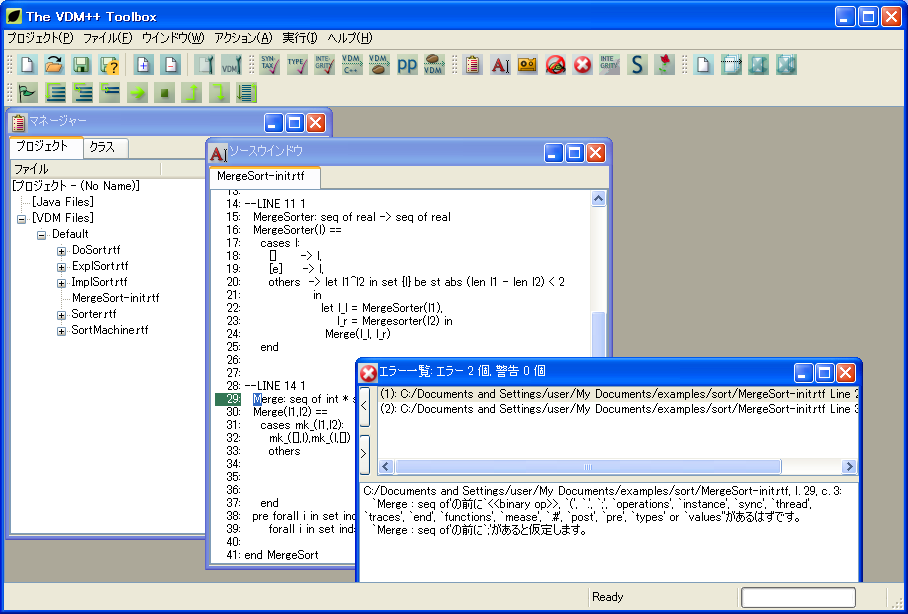
\includegraphics[width=11cm]{addedFiles-pp.png}
\caption{ファイル追加後のメインウインドウ}
\label{fig:addedfiles}
\end{center}
\end{figure}


\subsection{VDM仕様の構文チェック}\index{こうぶんチェック@構文チェック} 


プロジェクトを作成したら、すべての\ifthenelse{\boolean{VDMsl}}{モジュール}{クラス}が、\vdmslpp\ の
構文ルールに準じているかチェックする必要がある。構文チェック機能は、作成した仕様の構文が
正しいかどうかチェックする。プロジェクトにファイルを追加したり、プロジェクトに登録されている
ファイルが変更されたりすると、ツールは自動的に構文チェックを行う。ツールの設定で、自動的な
構文チェックを行わないようにすることもできるが、その場合は、
ファイルを変更したら、ツールの他の機能を使用する前に、再度構文チェックをしなくてはならないことを
忘れないでもらいたい。

\subsubsection{仕様の解析}


\guicmd{マネージャー}の\guicmd{プロジェクトビュー}で
\ifthenelse{\boolean{VDMsl}}{{\tt sort-init.rtf}ファイルをクリック}{6つの {\tt .rtf} ファイルを選択}し、 
(\guicmd{アクション})ツールバーの\raisebox{-0.7mm}{
\includegraphics[width=0.03\textwidth]{syntaxcheck.png}}  
(\guicmd{構文チェック})を押すと、構文チェック機能が起動する
(「Default」フォルダのレベルを選択し、構文チェックの操作を適用することで、
同じ操作を行うことができる。つまり、そのフォルダ内の各ファイルに操作が適用される)。
%ここで、\guicmd{ログウインドウ}が自動的に開き
%(すでに開いていない場合)、\ifthenelse{\boolean{VDMsl}}{``{\tt Parsing "sort-init.rtf" ...}''}{
%``{\tt Parsing "..../DoSort.rtf" ...}'' 等}のメッセージを表示することに注目してほしい。
\guicmd{ログウインドウ}に、\ifthenelse{\boolean{VDMsl}}{``{\tt Parsing "sort-init.rtf" ...}''}{
``{\tt Parsing "..../DoSort.rtf" ...}'' 等}のメッセージが表示されていることに、注目してほしい。
(ファイルは複数選択することもでき、その場合は選択されたファイルのすべての構文がチェックされる。)
\guicmd{ログウインドウ}には、エラー情報が出力されている場合があるので、問題解決の手がかりになることがある。
構文エラー\index{こうぶんエラー@構文エラー} が発見された場合は
\guicmd{エラー一覧}\index{エラーリスト}のウインドウが自動的に起動される。
また、\guicmd{ソースウインドウ} も表示される。
ソートのサンプルには、説明のために、二つ構文エラーがはいっている。

% \subsubsection{Traversing errors}
\subsubsection{構文エラーの修正}\index{こうぶんエラー@構文エラー!しゅうせい@修正}


図~\ref{fig:error}に\guicmd{エラー一覧}を示す。画面の上部に、エラーまたは警告の生じた
箇所のリスト(ファイル名、行番号、カラム番号)が表示され、下部には選択中のエラーの詳細情報が表示される。
最初はリストの先頭のエラーが自動的に選択される。

\begin{figure}[tbh]
\begin{center}
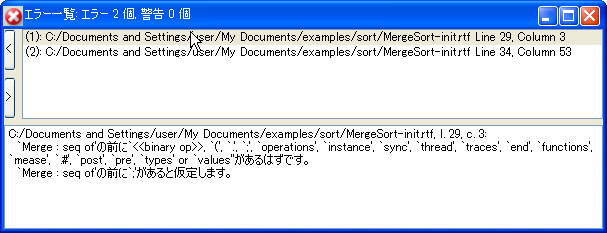
\includegraphics[width=\textwidth]{errorList-pp.png}
\caption{エラー一覧}
\label{fig:error}
\end{center}
\end{figure}

\guicmd{ソースウインドウ}には、エラー一覧内で選択中のエラーに対応する、仕様の部分が表示される。
実際の箇所は、ウインドウのカーソルでマークされて示される。最初の構文エラーに対しては、
\guicmd{ソースウインドウ}は図~\ref{fig:source1}のように表示される。

\begin{figure}[tbh]
\begin{center}
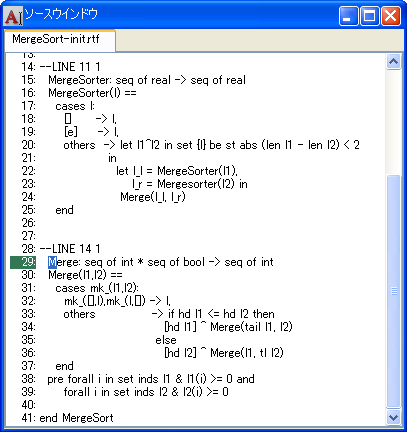
\includegraphics[width=9cm]{sourceWindow-pp.png}
\caption{最初のエラーがソースウインドウに表示された所}
\label{fig:source1}
\end{center}
\end{figure}

\newpage

最初のエラーメッセージは下記のとおり:

\begin{verbatim}
C:/Documents and Settings/user/My Documents/examples/sort/MergeSort-
    init.rtf, l. 29, c. 3:
  `Merge : seq of'の前に`<<binary op>>, `(', `.', `;', `operations',
    `instance', `sync', `thread', `traces', `end', `functions',
    `mease', `.#', `post', `pre', `types' or `values''があるはずです。
  `Merge : seq of'の前に`;'があると仮定します。
\end{verbatim}

この形式のメッセージは、エラーの発見されたポイントで、予測されるものが
見つからなかった場合に表示される。構文チェック機能は、エラーを報告し、
起こった箇所において、修正および構文チェックの続行を行うための仮説を示す。

この例では、エラーメッセージは、構文チェックを続けるためには、{\aaa Merge} 関数の
前に\Lit{;}が必要であるという仮説を伝えている。\cite{LangManPP-SCSK}を参照すれと、
\vdmslpp\  の構文の記述から、 この仮説が正しいことが分かる。すなわち、2つの関数定義は
デリミタ\Lit{;}で区切らなくてはならない。
このエラーは、{\aaa MergeSorter} 関数の定義の最後に、ファイルエディタを使って、
\Lit{;}という文字を追加することで修正できることがわかる。

(構文チェック機能が仮説を示しても、元ファイルは変更されないことに注意してほしい。
元ファイルの修正は、ユーザの手作業で行なわねばならない。)

構文エラーの修正は、\Toolbox\ 上から好みのエディターを直接起動する
ことで出来るようになる。(付録~\ref{sec:set_env}参照)メインウインドウで
\ifthenelse{\boolean{VDMsl}}{{\tt sort-init.rtf}}{{\tt MergeSort-init.rtf}}ファイルを選択し、
(\guicmd{ファイル})ツールバーの\guicmd{外部エディタ}\index{がいぶエディタ@外部エディタ} ボタン
(\raisebox{-0.8mm}{
\includegraphics[width=0.03\textwidth]{externaleditor.png}})を押す。
%外部エディタの起動時に複数のファイルが選択されていた場合、この方法だと選択したファイル
%それぞれが\guicmd{外部エディタ}で表示される。

エラーリストの左側に表示されている {\fbox{\tt >}}ボタンを押すか、\guicmd{エラー一覧}画面の画面上半分に
表示される、エラー箇所の概要を直接選択すると、見たいエラーリポートを読むことが出来る。以下のように説明がされている。


\begin{verbatim}
C:/Documents and Settings/user/My Documents/examples/sort/MergeSort-
    init.rtf, l. 34, c. 53:
  `l1 , l2 )'の前に`<<binary op>>, `(', `)', `,', `.', `[', `‾',
    `.#', ``' or `, ... ,''があるはずです。
  `l1 , l2 )'の前に`*'があると仮定します。
\end{verbatim}

これは{\tt l1, l2}の前で構文エラーが起こっており、構文エラーを修復
するためには、乗算記号`{\tt *}'が`{\tt tail}'と`{\tt l1}'の間に必要であるとの仮説を示して
いる(`{\tt tail}'は識別子の名前であると予測)。
この場合、仮説は間違っており、実際は、列から先頭を除いたものを返す`{\tt tl}'演算子を`{\tt tail}と
書き間違えたことによるエラーである。ファイルエディタを使って修正してみよう。

構文エラーを修正してファイルを保存したら、正しく修正できていることを確認するために、
再度構文チェック機能\index{こうぶんチェッカー@構文チェック機能}を走らせなくてはならない\footnote{標準の設定では、
外部エディタで仕様を修正し保存した後、\Toolbox\ のウインドウに戻ると、自動的に構文チェックが行われる}。
今回、仕様は構文的に正しいはずであり、
\guicmd{マネージャー} \ifthenelse{\boolean{VDMsl}}{}{の(\guicmd{クラスビュー})} 
内にある\vdmModView\ のウインドウを選ぶと、
\ifthenelse{\boolean{VDMsl}}{仕様を表すモジュール(この例ではモジュール構造を何も使用していないため、
{\tt DefaultMod} と呼ばれるモジュール)}{仕様で定義されている6つのクラス({\aaa
    DoSort, ExplSort, ImplSort, MergeSort, Sorter, SortMachine})}
の状態が確認できる。

さらに、構文的に正しいことを示す記号 \raisebox{-0.7mm}{
\includegraphics[width=0.03\textwidth]{syntaxcheckdone.png}}
が構文の欄についているはずだ。(図~\ref{fig:vdmModView}参照)
その他の欄がブランクなのは、仕様の型チェックやコード生成、清書などがまだ1度も行われていない
ことを意味している。

\begin{figure}[tbh]
\begin{center}
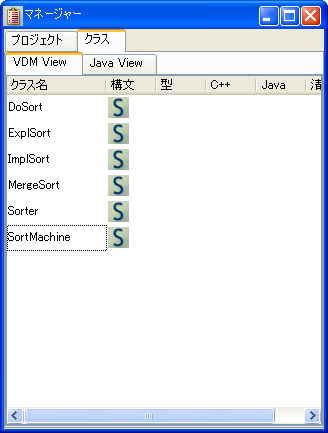
\includegraphics[width=9cm]{vdmView.png}
\caption{VDMビュー}
\label{fig:vdmModView}
\end{center}
\end{figure}

構文チェックが成功したので、ファイルを\vdmModView\ から直接選択して、次の処理に進むことができる。

\subsection{VDM仕様の型チェック}
\index{かたチェック@型チェック}\label{sec:gde-tc}


仕様が構文チェックをパスしたら、型チェックを行うことが出来る。
型チェックは(\guicmd{アクション})ツールバーの\raisebox{-1.0mm}{
\includegraphics[width=0.03\textwidth]{typecheck.png}}  
(\guicmd{型チェック}) ボタンを押すと起動する。

\vdmModView\ で \ifthenelse{\boolean{VDMsl}}{モジュール{\tt DefaultMod}}{6つのクラスすべて} 
を選択し、型チェックを行う。型チェックが終わると、 \Toolbox\ は、状態表示を更新し、記号
\raisebox{-1.0mm}{
\includegraphics[width=0.03\textwidth]{typecheckdone.png}}
と\raisebox{-1.0mm}{
\includegraphics[width=0.03\textwidth]{typecheckerror.png}}
(赤いラインのついた\raisebox{-1.0mm}{
\includegraphics[width=0.03\textwidth]{typecheckdone.png}})
を使って、各々の\ifthenelse{\boolean{VDMsl}}{モジュール}{クラス}に関して型チェックが成功したか失敗したかを示す。

この例では、説明のために、
\ifthenelse{\boolean{VDMsl}}{Sortの仕様}{{\tt MergeSort}クラス}
の型チェックが失敗するようになっている。エラーが4つ\footnote{型エラーのフォーマットに
ついては、このマニュアルのリファレンス部分に詳細が記述されている。セクション~\ref{type check}
参照}と警告が1つ発生しする。これらは、構文エラーと同様、\guicmd{エラー一覧} に表示される。

図~\ref{fig:type_error1}に示されている最初のエラーは、
関数名{\tt Merge\underline{s}orter} の{\tt s}が小文字であることが原因である。
(\guicmd{ソースウインドウ} の表示については図~\ref{fig:source-type}を参照のこと)
この関数名は {\tt MergeSorter}でなくてはならない。


\begin{figure}[tbh]
\begin{center}
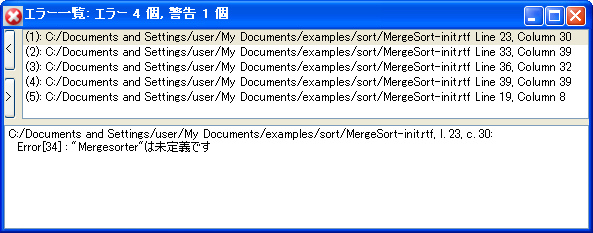
\includegraphics[width=11cm]{typeError1-pp.png}
\caption{型チェック後最初のエラー表示}
\label{fig:type_error1}
\end{center}
\end{figure}

\begin{figure}[tbh]
\begin{center}
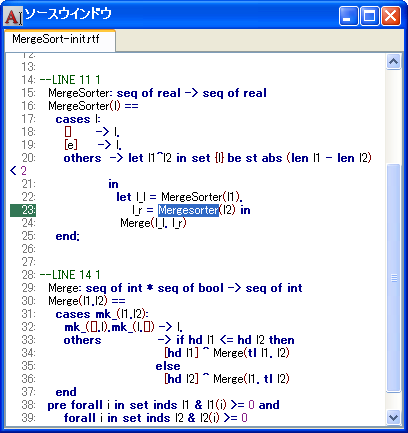
\includegraphics[width=9cm]{sourceWindow-type-pp.png}
\caption{型エラー時のソースウインドウ}
\label{fig:source-type}
\end{center}
\end{figure}


図~\ref{fig:type_error2}に示される2番目のエラーは、
数値型でない右辺に\Sig{<=}演算子を適用しようとしたために起きたものである。
もっと詳しく言えば、期待される引数の型(エラーメッセージ中では{\sf exp:}と表示)が{\tt real}型
(実数型は最も一般的な数値の型である)であるのに対して、実際の引数の型
(エラーメッセージ中では{\sf act:}と表示)は{\tt bool}型であるため型の不整合が生じている。
エラーの原因を特定しようとする場合、このような情報は有用な場合がある。

\begin{figure}[tbh]
\begin{center}
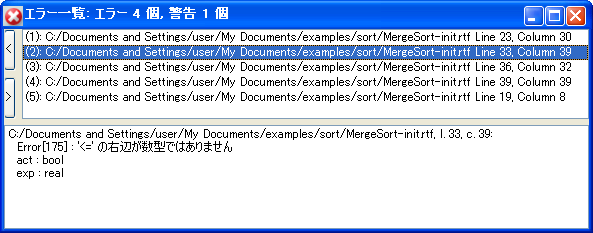
\includegraphics[width=11cm]{typeError2-pp.png}
\caption{2番目の型チェックエラー表示}
\label{fig:type_error2}
\end{center}
\end{figure}


このエラーは、{\tt Merge}関数のシグネチャに、{\tt seq of int}で
あるはずのものが{\tt seq of bool} と書かれていることが原因である。
\ifthenelse{\boolean{VDMsl}}{3番目のエラーも\Sig{<=} 演算子の左辺が右辺となっているだけで、同様である。
そのため、これらのエラーは、最初のエラーに関連して出たものである。最初のエラーを
修正して}{3番目と4番目のエラーも同じ原因であり、2番目のものとも関係しているため、2番目のエラー
が修正されると消える。このため、最初の2つのエラーを修正して} 
、再度、仕様の構文チェック、型チェックを行う。 

メインウインドウの状態についての情報が、この処理中どのように更新されたか注目してほしい。
まず元ファイルが編集されると、\vdmModView\ でそのファイルが構文的に正しいことを示す記号
\raisebox{-0.7mm}{
\includegraphics[width=0.03\textwidth]{syntaxcheckdone.png}}  
が、\Toolbox\ 上に現在あるバージョンとファイルシステムにあるバージョンの不整合があることを示す
\raisebox{-0.7mm}{
\includegraphics[width=0.03\textwidth]{syntaxcheckmodified.png}}に変わる\footnote{自動構文
チェックによりこの記号をみることはないかもしれない}。
このファイルは、処理を行う前に再度構文チェックが行われていなくてはならない。次に、構文チェックの後、
再度型チェックを走らせると、両方の処理が正しく終了したことを示す記号
\raisebox{-0.7mm}{
\includegraphics[width=0.03\textwidth]{syntaxcheckdone.png}}と
\raisebox{-1.0mm}{
\includegraphics[width=0.03\textwidth]{typecheckdone.png}} 
がそれぞれの状態表示する場所に表示される。

型チェック処理は、警告を返してきたとしても成功であることに注意。
これは警告は、通常、実際のエラーではなく、仕様の中の冗長性を示している。
例えば、あるブール式がいつもfalseであると予想されたり、
特定のパラメータやローカル変数が関数や操作中で一度も使用されないなどである。
もちろん、このような冗長性は、実際のエラー(警告を出している式や文にタイプミスがあるような)に起因するかもしれない。
そのため、警告をチェックすることは、そのようなことがないかどうかを確認するためにも有用である。
例では、{\tt MergeSort} 関数内のcases式の2番目のパターンにあるローカル変数`{\tt e}'が、
一度も使用されていないという警告が表示されている。これは、現実には、エラー
ではなく、仕様は正しく意味をなしている。ただし、警告を除去したいのであれば、
`{\tt e}'を`{\tt -}'(“don't-care” pattern)に置き換えればよい。

仕様が型チェックをパスしても、正しいことを保障するものではなく、まだエラーが潜んでいるかもしれない
(なんらかのプログラミング言語のコンパイラの構文チェック、型チェックをパスしたとしても、
0除算によるランタイムエラーなどがありうるように)。このような、モデル中のランタイムエラーの
元となりうる潜在的なところを特定する一助とするために、型チェック機能には、
仕様中でランタイムエラーを起こしうる潜在的なところをすべてエラーとして報告するオプションがある。
%そのため、もし報告された潜在的なエラーが起こり得ないと自分自身が納得するなら、
%ランタイムエラーは起こらないだろう。
このオプションについての情報は、マニュアルのセクション~\ref{sec:def-typechedk}を参照のこと。

% Ueki 2005/01/06 ここまで

% 
% %%%%%%% Next bit needs reinstating and updating when References
% %%%%%%% window is working -- RM 
%
% #ifdef 
% \subsection{Getting an Overview of the Classes}

% {\bf whole section needs revising -- RM}

% It can be difficult to gain an overview of the structure of a \vdmpp\ 
% specification simply from its ``flat'' documentation. The \Toolbox\ 
% includes two tools which can show the structure of the classes which
% have been read in and syntax checked.  These are called the
% \guicmd{Inheritance Tool} and the \guicmd{Dependency Tool}.
% Alternatively, if you prefer to use UML, the Rose-\vdmslpp\ link could
% be used instead. However, that link will not be considered in this
% manual, instead we refer the interested readers to \cite{UMLMan-SCSK}.
% % (see \cite{} for more information).

% \subsubsection{Using the inheritance tool}

% Invoke the \guicmd{Inheritance tool}\index{Inheritance Tool} from the
% \guicmd{Tools} menu in the main window. The inheritance tree of the
% sort specification will now appear in a new window as shown in
% Figure~\ref{fig:inhtree}. The inheritance tree shows that {\tt Sorter}
% is a superclass of {\tt DoSort}, {\tt ExplSort}, {\tt ImplSort} and
% {\tt MergeSort}. The {\tt SortMachine} class has no super- or
% subclasses. The tool gives the inheritance information of those
% classes that have been accepted by the syntax checker.

% \begin{figure}[tbh]
% \begin{center}
% %\resizebox{8cm}{!}{\includegraphics{inhtree}}\
% \caption{The Inheritance Tree of the Sorting Specification\label{fig:inhtree}}
% \end{center}
% \end{figure}

% Besides giving a survey of the inheritance structure of the
% specification, the inheritance tree can also be used to navigate
% through your specification. Select one class in the inheritance tree
% by clicking with the leftmost mouse button. The class will now be
% selected in the main window of the \Toolbox.


% \subsubsection{Using the dependency tool}\label{sec:dependencytool}

% Another way to get a better overview of the structure of a \vdmpp\ 
% specification is to use the \guicmd{Dependency Tool}\index{Dependency
%   Tool} which for a selected class shows:
% \begin{itemize}
% \item its superclasses, 
% \item its subclasses, 
% \item the classes it uses~(a class {\em uses\/} another class if it
%   has references to objects of that class, for example through its
%   instance variables or operation calls), and
% \item the classes which use the selected class.
% \end{itemize}

% Select the \guicmd{Dependency Tool} in the \guicmd{Tools} menu bar in
% the main window. A new window with the \guicmd{Dependency Tool} will
% now pop up. If you select the class {\tt Sorter} in the classes list
% in the main window the \guicmd{Dependency tool} will appear as shown
% in Figure~\ref{fig:dep_sorter}. You can see that {\tt DoSort}, {\tt
%   ExplSort}, {\tt ImplSort} and {\tt MergeSort} are subclasses to the
% {\tt Sorter} class and that the {\tt Sorter} class uses the {\tt
%   SortMachine} class (the {\tt SortMachine} has an instance variable
% which is an object reference to the {\tt Sorter} class).


% \begin{figure}[tbh]
% \begin{center}
% %\resizebox{9cm}{!}{\includegraphics{dependency_sorter}}
% \caption{The Dependency Information on the {\tt Sorter} Class\label{fig:dep_sorter}}
% \end{center}
% \end{figure}

% As with the \guicmd{Inheritance Tool}, you can navigate through the
% specification in the \guicmd{Dependency Tool}. Just click on a class
% in the \guicmd{Dependency Tool} and that class will be selected
% in the main window, in the \guicmd{Dependency Tool} and in the
% \guicmd{Inheritance Tool} if it is open. Now try clicking on class
% {\tt SortMachine}, and you will get the dependency information for
% this class as shown in Figure~\ref{fig:dep_sortmachine}. From this you
% can see that the class has no super- or subclasses, nor is it used by
% any other classes, however, it uses the class {\tt Sorter}.


% \begin{figure}[tbh]
% \begin{center}
% %\resizebox{9cm}{!}{\includegraphics{dependency_sortmachine}}
% \caption{The Dependency Information on the {\em SortMachine} Class\label{fig:dep_sortmachine}}
% \end{center}
% \end{figure}
% #endif //

\subsection{仕様の検証}


仕様はある目的のために作成される:通常は、提案されたコンピュータシステムの
設計された振る舞いの理解を深めるためや、安全性などの特性を考慮して
設計されているかチェックするため、次の詳細設計や実装の基礎に役立てる
ためなどだ。その目的は何であれ、単に仕様の構文や型が正しいだけでは
不十分で、たとえ抽象的なレベルであっても、モデル化されたシステムの振る舞いを
忠実に表現していなくてはならない。

{\em 検証\/}は形式仕様が、モデル化されたシステムの非形式に表現された
要求を正確に反映しているかどうかについて自信を深めるプロセスである。
形式仕様言語の仕様があれば、広範囲の検証技術が使える:仕様は
詳細に調べることができ、テストもできる。仕様が設計された特徴を表現して
いるかについて極めて厳格な試験を実施することも可能だ。\Toolbox\ はアニメーションと
デバッガ(仕様の一部に値を入力して実行)とインタープリタを使ったテストまで、
あるいは証明課題の生成まで検証作業をサポートしている。このセクション
では仕様のチェックとその品質向上のために使われるインタープリタ、デバッガや
証明課題生成機能をどう使うかについて記述する。

\subsubsection{インタープリタを使用した式の評価}
\label{interpreter}\index{インタープリタ}


インタープリタを使って、式や文の評価とデバッグを行うことができる。
これらはかなり複雑で、\Toolbox\ に読み込まれている仕様で定義されている
関数や操作の実行、変数の使用を含んでいる。デバッガを使って
ブレイクポイントの設定、評価作業のステップ実行、変数の値を見るなどができる。

図~\ref{fig:interpwin}に示す\guicmd{実行ウインドウ}\index{インタープリタウィンドウ}が、
(\guicmd{ウインドウ})ツールバーの\raisebox{-1.0mm}{
\includegraphics[width=0.03\textwidth]{interpreter.png}}  
(\guicmd{実行})ボタンを押すことによって開く。
\guicmd{実行}ツールバーが、まだ開いていなければ同時に開く。


\begin{figure}[tbh]
\begin{center}
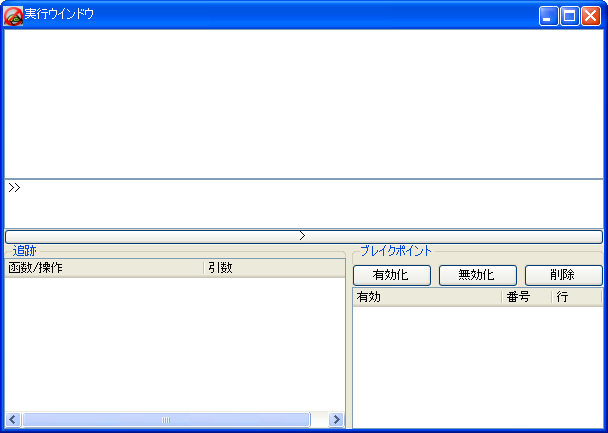
\includegraphics[width=11cm]{interpreterWindow.png}
\caption{実行ウインドウ}
\label{fig:interpwin}
\end{center}
\end{figure}


実行ウインドウの上部には2つの画面、それぞれ\guicmd{応答} と\guicmd{入力}画面がある:
\guicmd{入力}画面からはインタープリタに直接コマンドを入れることが出来、
その結果が\guicmd{応答}画面に表示される。\vdmslpp\ の式を評価するためには、
\guicmd{入力}画面からコマンドラインで直接タイプする。 

入力画面で下記のようにタイプしてみよう:

\begin{verbatim}
  print { a | a in set {1,...,10} & a mod 2 = 0 }
\end{verbatim}

Returnキーを押す。
答えとして、偶数の集合が表示される。今検証した式は、集合内包と呼ばれる構成子
である。後に(\ifthenelse{\boolean{VDMsl}}{\cite{UMLMan-SCSK}}{\cite{LangManPP-SCSK}})で説明する。

\raisebox{-1.0mm}{
\includegraphics[width=0.03\textwidth]{runI.png}}  
(\guicmd{初期化})ボタンを押すことで、 インタープリタの初期化\index{インタープリタ!しょきか@初期化}
が行われ、\ifthenelse{\boolean{VDMsl}}{{\tt sort-init.rtf} ファイル}{仕様ファイル}から読み込まれている
\vdmslpp\ の構成要素を参照することが可能になる。
初期化中に、定数は評価され、\ifthenelse{\boolean{VDMsl}}{状態定義の値}{インスタンス変数}が初期化される。
初期化後は、関数、操作、
インスタンス変数、値、型など仕様\ifthenelse{\boolean{VDMsl}}{}{のクラス}内で定義されているものなら
何でも参照できる。 


どの関数が{\aaa MergeSort}クラスから呼び出し可能かを見るために、\guicmd{入力} 画面の
プロンプトで{\cmd functions MergeSort} とタイプする。そうすると、{\aaa MergeSort}クラスの
呼び出し可能な関数のリストが表示される。リストからは関数{\aaa pre\_Merge}のような、
付随する事前条件がある場合に生成される事前条件関数
\index{じぜんじょうけんかんすう@事前条件関数 |see{\\ 関数, \\ 事前条件}}
\index{かんすう@関数!じぜんじょうけん@事前条件}
を呼び出すことが可能であることがわかる。

関数や操作の適用、インスタンス変数や値 (定数) 定義の精査は、
オブジェクトを通じてのみ実行される。オブジェクトを生成すれば、
インタープリタ内でそれらを利用することがが可能となる。

以下の2つのコマンドは、\guicmd{入力} 画面で使うと、{\aaa ms} という名の {\aaa MergeSort}クラスの
オブジェクトを生成し、引数[3, 56, 34-12, 0 ] で{\tt ms} の{\tt Sort}関数を呼び出し、
結果を表示する。

\begin{verbatim}
  create ms := new MergeSort()
  print ms.Sort([ 3, 56, 34-12, 0 ])
\end{verbatim}

また、オブジェクトはインタープリタ中の記述の評価中でもローカルに生成することが
可能である。例えば、前の例の{\tt ms}オブジェクトのようにオブジェクト名をつけなくても
{\tt MergeSort`Sort}は以下のコマンドで実行できる 

\begin{verbatim}
  print new MergeSort().Sort([ 3, 56, 34-12, 0 ])
\end{verbatim}

この例では、評価の期間中はローカルにオブジェクトが生成される。すなわち、{\tt Sort} 操作
のテスト中だけオブジェクトが存在することとなる。

インスタンス変数を調べるため、まず {\tt SortMachine}クラスのオブジェクトを生成する。

\begin{verbatim}
  create sm := new SortMachine()
\end{verbatim}

{\tt SortMachine}クラスは{\tt srt}という名前のインスタンス変数を持ち、これは{\tt Sorter}
オブジェクトへの参照である。最初から{\tt srt}は{\tt MergeSort}オブジェクトを指している。
まず、{\tt srt}の値を見てみてから、それが指しているオブジェクトの{\tt Sort}操作を呼んでみよう。

\begin{verbatim}
  print sm.srt
  print sm.srt.Sort([ 3, 56, 34-12, 0 ])
\end{verbatim}

図~\ref{fig:evalgui}は上記の評価の結果を示している。


\begin{figure}[tbh]
\begin{center}
\mbox{}
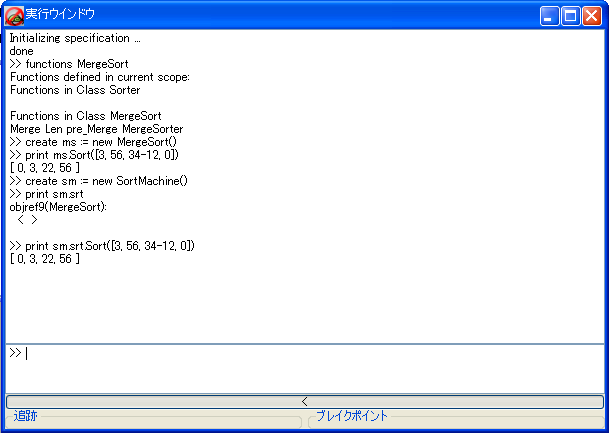
\includegraphics[width=15cm]{evalExpr-pp.png}
\caption{式の評価}
\label{fig:evalgui}
\end{center}
\end{figure}


\vdmslpp\ の構成要素すべてが実行可能なわけではないので、実行可能でない
ものはインタープリタを使った評価が出来ないことに注意。例えば、陰関数{\aaa ImplSort`ImplSorter} を
数字の引数を使って呼び出そうとした場合、インタープリタは評価中に実行不可能な構成要素
\index{じっこうふかのうなこうせいようそ@実行不可能な構成要素}に出くわしたとエラーを返す。
図~\ref{fig:evalgui}を参照

\subsubsection{ブレイクポイントの設定}
\label{sec:gui-breakpoints}\index{ブレイクポイント}\index{ブレイクポイント!せってい@設定} 

ブレイクポイントは、インタープリタで関数などの実行をするときに実行を一時中断する。

\ifthenelse{\boolean{VDMsl}}{{\aaa break MergeSort}}{{\aaa break MergeSort`MergeSorter}}
とタイプすることで、
\ifthenelse{\boolean{VDMsl}}{関数{\aaa MergeSort}}{クラス{\aaa MergeSort} の関数{\aaa MergeSorter}}
にブレイクポイントを設定することができる。

(\ifthenelse{\boolean{VDMsl}}{現在のモジュールにブレイクポイントを設定するときは、単純に関数または操作
名を参照すればよい。他モジュールにブレイクポイントを設定する場合は、関数または
操作名を定義済みのモジュール名で修飾しなくてはならない。}{
ブレイクポイントを設定するときは、関数や操作の名前を、それらが定義されているクラス名で修飾しなければ
ならない。})
コマンドを実行すると、\guicmd{実行ウインドウ}の右下の\guicmd{ブレイクポイント}画面に、
ブレイクポイントに割当られた番号(この場合、最初にブレイクポイントを設定しているので1)、
ブレイクポイントが有効であることを示す印 \raisebox{0.5mm}{{\fbox{\tt\tiny $\surd$}}}とともに、
ブレイクポイントの設定場所が表示される。
今度は、以前使った\index{printコマンド}コマンドを使う代わりに、{\cmd debug}コマンドを使って評価作業を行うことが
出来る。この2つのコマンドの違いは、{\cmd print} がブレイクポイントを無視する一方、{\cmd debug}コマンド
はブレイクポイントでインタープリタを停止させることができることである。\index{ブレイクポイント!むし@無視}

以下のようにタイプして
\ifthenelse{\boolean{VDMsl}}{{\aaa MergeSort}}{{\aaa Sort}}関数を呼び出してみよう。

\begin{verbatim}
  debug new MergeSort().Sort([ 3, 56, 34-12, 0 ])
\end{verbatim}

インタープリタは\ifthenelse{\boolean{VDMsl}}{{\aaa MergeSort}}{{\aaa Sort}}
関数に入ったところのブレイクポイントでストップする。
同時に、
\ifthenelse{\boolean{VDMsl}}{{\aaa MergeSort}}{{\aaa Sort}}
関数を含む仕様のソースファイルが\guicmd{ソースウインドウ}に表示され、
現在評価中のポイント(ここではブレイクポイントの場所。例では
\ifthenelse{\boolean{VDMsl}}{{\aaa MergeSort}}{{\aaa Sort}}
関数の最初のところ)
にカーソルが当たる。加えて、\guicmd{追跡}画面(\guicmd{実行ウインドウ}の左下)には
コールスタック\index{コールスタック}が表示される。

ここで、\ifthenelse{\boolean{VDMsl}}{{\aaa MergeSort}}{{\aaa Sort}} 
{\cmd print}コマンドを使う(\guicmd{入力}画面で{\aaa print l} とタイプする)\index{printコマンド}か、
\guicmd{実行ウインドウ}の左下部分にある\guicmd{追跡} 画面の関数名の近くに表示されている\Sig{...} 部分を
マウスの左ボタンをクリックするかすると、関数のパラメータの値を詳細に見ることが出来る。
値の表示されているパラメータ上でマウスの左ボタンをクリックすると、また\Sig{...} 表示に戻る

ソースファイルの箇所を直接選択することでもブレイクポイントを設定することができる。
加えて、ブレイクポイントは関数・操作の最初である必要はなく、その内部であればどこでも設定できる。

ソースファイルがRTF形式のファイルでない場合は、
\guicmd{ソースウインドウ}のファイル中の設定したい位置で右ボタンをクリックし、
メユーから\guicmd{ブレイクポイント設定}を選択することで、ブレイクポイントを設定できる。
ソースファイルにRTFフォーマットを使っている場合は、Wordでファイルの適切な位置に
カーソルをあて\texttt{Control-Alt-Spaceキー} でブレイクポイントが設定できる。

デバッグ中はいつでもブレイクポイントが設定できる。それでは、上記の方法で、ソースファイルを使って、
\ifthenelse{\boolean{VDMsl}}{}{{\aaa MergeSort}クラスの}
{\aaa Merge}関数内にブレイクポイントを設定してみよう。

インタープリタに戻って(\guicmd{実行})ツールバーの
\raisebox{-1.0mm}{
\includegraphics[width=0.03\textwidth]{continueI.png}} 
(\guicmd{実行再開})ボタンを押してみよう。これで
次のブレイクポイントまで実行される。実際には
\ifthenelse{\boolean{VDMsl}}{{\aaa MergeSort}}{{\aaa Sort}}
の再帰的な呼び出しによって、インタープリタは同じブレイクポイントで何度か止まるが、
そのたびに{\tt Merge}関数の中で実行がとまるまで\guicmd{実行再開}ボタンを何度も押す。

実行が進むにつれ、さまざまな関数が呼ばれ\guicmd{追跡}画面にログが増えていく。
そしてこのコールスタック\index{コールスタック} を実行のステップをトレースするのに使うことが出来る。 
\raisebox{-1.0mm}{
\includegraphics[width=0.03\textwidth]{upI.png}}  
(\guicmd{一段上の函数の呼び出し位置を表示})ボタンを何度か押して関数のトレースの前後関係がどう変化しているか確認できる。 
\raisebox{-1.0mm}{
\includegraphics[width=0.03\textwidth]{downI.png}}  
(\guicmd{ー段下の函数の呼び出し位置を表示})ボタンは追跡を元に戻すときに使う。

\raisebox{-1.0mm}{
\includegraphics[width=0.03\textwidth]{singlestepI.png}}
(\guicmd{1ステップ実行})ボタンを押すことでステップ実行をすることもできる。ボタンを何度か押して、
\guicmd{ソースウインドウ} 中のカーソルが、評価箇所の変化をマークする様子を確認してほしい。
これで、関数のパラメータだけでなく、スコープ中にあるローカル変数を含むすべての変数に
アクセス可能になった。さらに、例えば{\cmd print} コマンドを使うことなどで、値の中身を見ることもできる
ようになった。

図~\ref{fig:guidebug}にデバッグの例を示す。

\begin{figure}[tbh]
\begin{center}
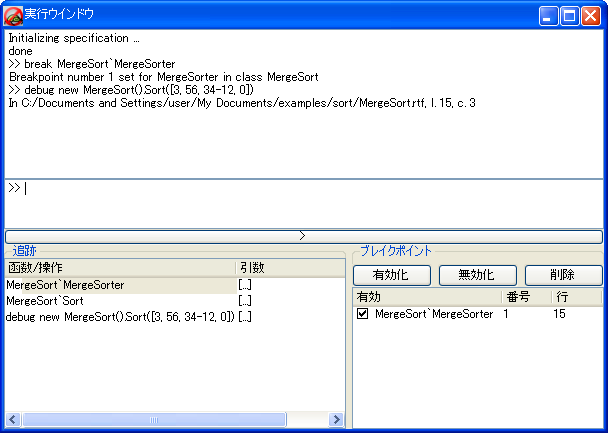
\includegraphics[width=15cm]{debugging-pp.png}
\caption{仕様のデバッグ}

\label{fig:guidebug}
\end{center}
\end{figure}


ブレイクポイントは、デバッグ実行中であってもなくても、いつでも削除することができる\index{ブレイクポイント!さくじょ@削除}。
\guicmd{実行ウインドウ}の\guicmd{入力} 画面で\\
{\tt delete 1} (例\ ブレイクポイント1番を削除)\\
とタイプしてみてほしい(これで1番のブレイクポイントが削除される)。
\guicmd{実行ウインドウ}の\guicmd{ブレイクポイント}画面で、ブレイクポイントを選択して画面上部
にある\guicmd{削除}ボタンを押しても結果は同じである。

\guicmd{ブレイクポイント} 画面上部の他2つのボタンは、ブレイクポイントの有効・無効を設定する。
\index{ブレイクポイント!むこう@無効}\index{ブレイクポイント!ゆうこう@有効}
\ifthenelse{\boolean{VDMsl}}{{\aaa MergeSort}}{{\aaa MergeSort`MergeSorter}}関数
の中にブレイクポイントを再度設定し、それを
\guicmd{ブレイクポイント}画面で選択して\guicmd{無効化}ボタンを押してみよう。
記号
\raisebox{0.5mm}{{\fbox{\tt\tiny $\surd$}}}\
がブレイクポイントが無効になっていることを示す
\raisebox{1mm}{{\fbox{\rule[-0.75mm]{0mm}{1.5mm}{\hspace*{1.5mm}}}}}\ 
に変わっていることに注目。\guicmd{有効化} ボタンを押すことでブレイクポイントは再度有効になり、記号は
\raisebox{0.5mm}{{\fbox{\tt\tiny $\surd$}}}\ 
に戻るはずである。

% It is also possible to make
% nested debugs.\index{Debugging!Nested} Try doing this and try using the
% {\tt popd}\index{{\tt popd} command} command to restore the context
% that existed when the last {\tt debug} command was invoked.

\subsubsection{動的型チェック}
\index{かたチェック@型チェック!どうてき@動的}

型チェック機能が仕様のエラーを報告しなくても、型情報の簡単な静的解析(関数や操作の
シグネチャに宣言されている型のみに基づいた解析)では、
通常、すべての型エラーを見つけることは不可能なので、型エラーが存在する可能性がある。
例えば、ある関数の引数が1個の整数({\aaa int}型)と定義され、
実数({\aaa real}型)に対して評価する式が適用されていたとしても、
{\aaa int} 型が{\aaa real}型のサブタイプであるため、関数の実行時に、整数値を持つ実数型の引数で
関数が呼ばれた場合、その適用は正しい。

仕様レベルでこの手の型エラーを発見するために、評価実行中に、インタープリタが
動的型チェックを実行するよう設定することができる。
このオプションは\guicmd{プロジェクトオプション} ウインドウの\guicmd{実行} タブで設定できるが、プロジェクト
オプションツールバーに表示されている\raisebox{-1.0mm}{
\includegraphics[width=0.03\textwidth]{projectoptions.png}} 
 (\guicmd{プロジェクトオプション} )ボタンを押すことで当該画面が表示される。
下記図~\ref{fig:interoptions}にこれを示す。

\begin{figure}[tbh]
\begin{center}
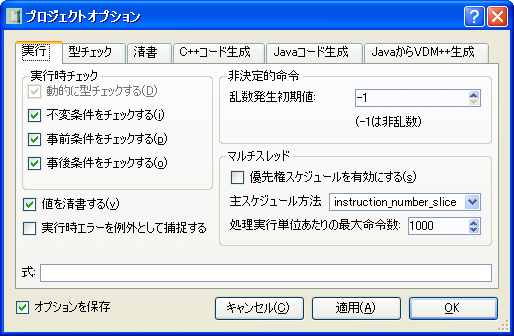
\includegraphics[width=12.5cm]{interpreterOptions-pp.png}
\caption{インタープリタオプションの設定}
\label{fig:interoptions}
\index{Options!Interpreter}
\end{center}
\end{figure}


「動的に型チェックする」オプションをを有効にすると、インタープリタは評価実行中、実際の型をチェックする。

今回の例では、\guicmd{プロジェクトオプション}ウインドウの\guicmd{実行} タブで動的型チェックを有効に設定し、
\guicmd{適用} 、\guicmd{OK} ボタンを押すと 、式の評価


\begin{verbatim}
  debug new MergeSort().Sort([ 3.1415, -56, 34-12, 0 ])
\end{verbatim}

のところでインタープリタは動的型チェックエラーを報告する。(ブレイクポイントを有効に
設定したままになっていた場合は、一度ステップ実行をする必要がある)これは、関数
\ifthenelse{\boolean{VDMsl}}{{\aaa Merge}}{{\aaa MergeSort`Merge}}
のシグネチャが、引数にint型をとると宣言してあるのに、
実際の引数は{\tt 3.1415}というreal型(int型でない)の数字を含んでいるからである。この動的
型エラーは、仕様のエラーの可能性を明らかにしている−
\ifthenelse{\boolean{VDMsl}}{}{ {\aaa MergeSorter} クラスの}
{\aaa MergeSort}関数はパラメータとしてreal型の列も許容すべきなのに、
\ifthenelse{\boolean{VDMsl}}{}{同じクラスの}
integerの列のみを許容する{\aaa Merge} 関数を呼び出しているためだ。

似たような方法で、インタープリタが動的に型の不変条件や関数の事前条件、事後条件、
予想される操作(例\ {\aaa true}と評価される)などのチェックをするように設定することが
可能である。これらのオプションも図~\ref{fig:interoptions}.\index{じぜんじょうけんチェック@事前条件チェック}
\index{じごじょうけんチェック@事後条件チェック}\index{ふへんじょうけんチェック@不変条件チェック} にあるような
\guicmd{プロジェクトオプション} ウインドウの\guicmd{実行} 
タブで設定することができる。

例として\guicmd{プロジェクトオプション} ウインドウの\guicmd{実行} タブに戻って、
\guicmd{事前条件をチェックする}のオプションチェックを有効にしてみよう。これで以前の箇所を再度評価してみると、
今度はリストから数字{\tt 3.1415}が省略されてしまっている。今度はインタープリタが図~\ref{fig:dtcerror}に示す
ように事前条件違反を報告している。これは
\ifthenelse{\boolean{VDMsl}}{{\aaa Merge}}{{\aaa MergeSort`Merge}}関数の事前条件が、
入力値の全てが負でないことを要求しているからだ。

\begin{figure}[tbh]
\begin{center}
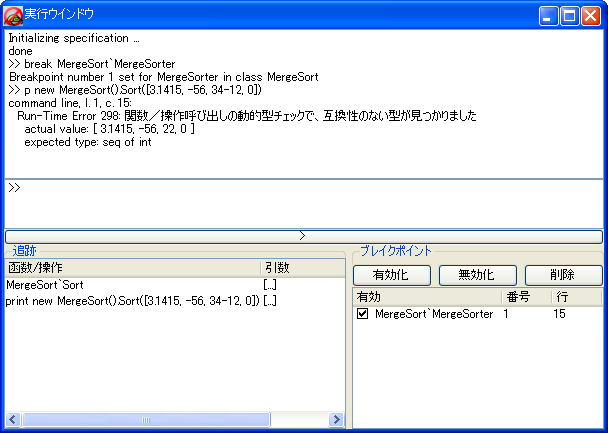
\includegraphics[width=12.5cm]{dynamicTCError-pp.png}
\caption{動的型チェックエラー}
\label{fig:dtcerror}
\end{center}
\end{figure}

\subsubsection{証明課題のチェック}\label{pogWalk}
\index{しょうめいかだい@証明課題}

上記の型チェック、不変条件、事前条件、事後条件などの動的チェックは
基本的にテストの一形式である−いくつかの \emph{特別な}入力値に対してランタイム
エラーが起こるかどうかチェックする。証明課題生成機能はランタイムエラーの可能性を
調査するもっと一般的な方法を提供するが、これは数学よりもプログラミングに
通じている人からすれば、あまり直感的に理解できないかもしれない。

証明課題生成機能は仕様の潜在的にランタイムエラーが起こりうる箇所を探して分析し、
ランタイムエラーが起こりえない条件を表す一連の証明課題を生成する。
これらの証明課題は、動的チェックよりもより一般的に使われるが、それは適切な
変数\footnote{
場合によっては、すべてのコンテクストが明確に示されず、変数のスコープが仕様の精査によって定義される。
}がとりうる
すべての値の定量化を含む \vdmslpp\ の記述として表現されるからである。
これは、もし証明課題がTrueと実行された場合、変数の値に何が入っていようが
それと関連するランタイムエラーは存在しないことになる(動的チェックの場合、
もちろん選ばれた変数の特定の値についてランタイムエラーが起こらないことが確認できる
にすぎない)。もちろん、証明課題がfalseを示すこともあり、その場合仕様の
相当する箇所に潜在的な問題があることを指摘している。

実際に証明課題生成機能がどう動くかを見るには、
\ifthenelse{\boolean{VDMsl}}{{\aaa DefaultMod} モジュール}{ {\aaa
    ExplSort} クラス} を選択し
(\guicmd{アクション})ツールバーの\raisebox{-1.0mm}{
\includegraphics[width=0.03\textwidth]{integritycheck.png}}  
(\guicmd{証明課題生成})ボタンを押すとこの
\ifthenelse{\boolean{VDMsl}}{モジュール}{クラス}の整合性
テスターが起動する。\guicmd{証明課題ウインドウ}が開いて表示され、証明課題が
生成される。図~\ref{fig:integWin}にこれを示す。


\begin{figure}[tbh]
\begin{center}
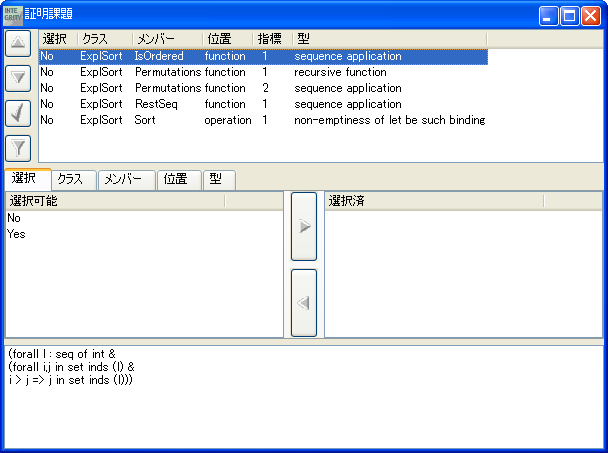
\includegraphics[width=12.5cm]{integWin-pp.png}
\caption{証明課題ウインドウ}
\label{fig:integWin}
\end{center}
\end{figure}


\guicmd{証明課題ウインドウ}の画面上部に証明課題のリストがそれらの状態
(\guicmd{選択済} 欄)、仕様の場所(\guicmd{モジュール}、 \guicmd{メンバー} 、 \guicmd{位置} 欄)と型(\guicmd{型}欄)
の情報と一緒に表示されている。\guicmd{指標} 欄の数字は単純に同じ箇所の違う証明課題
を区別するものである。この例でも見られるように、小さい仕様であっても、
たくさんの証明課題を生成することがある−実際、30ある証明課題の
すべてがチェックされている−そのため、大きな仕様ではこれらをフィルターできるため、
有効である。
\guicmd{証明課題ウインドウ} の中ほどの2つの画面で、さまざまなフィルタリング方法が
利用できる
\ifthenelse{\boolean{VDMsl}}{}{ (詳細はセクション~\ref{sec:pog} 参照)。}
最後に、特定の証明課題がウインドウ
のトップ画面で選択されると、それに相当する\vdmslpp\ の記述がウインドウの下の画面に
表示され、同時に\guicmd{ソースウインドウ} のカーソルが仕様の関連する箇所を示す。
それぞれの証明課題はTrueかそうでないかを決定しようとするため、詳細に調べられる。



{\aaa isOrdered}関数と関連する最初の証明課題(例\ インデックス番号1番)を選
択してみよう。これは下記のような形式になっている:


\begin{verbatim}
  (forall l : seq of int &
  (forall i,j in set inds (l) &
  i > j =>
   i in set inds (l)))
\end{verbatim}


そして\guicmd{ソースウインドウ}のカーソルの位置から、\verb+l(i)+ で表されるシーケンス
 アプリケーションの状態と関連していることがわかり、

\begin{verbatim}
  forall i,j in set inds l & i > j => l(i) >= l(j)
\end{verbatim}

は正しい定義である(例:\ {\aaa i}の値は常に列{\aaa l}のインデックス)。

このような典型的な例では、実際証明課題が正しいことを見て取るのは
簡単だが - 2番目の記述は、直接的には{\aaa i}も{\aaa j}も{\aaa l}のインデックスであることを示しており、
{\aaa i}が{\aaa j}より大きいかどうかに関わらず(3行目の記述)不適切であるとされている。
それゆえ、この課題はチェックしなくてはならない。\guicmd{証明課題ウインドウ}の
トップ画面左の \raisebox{-1.0mm}{
\includegraphics[width=0.03\textwidth]{checkmark.png}}
(\guicmd{項目の選択/非選択}) ボタンを押すことによってチェックができる。

列 アプリケーションに関連する他の3つの証明課題を見てみよう。
これらが正しいことを確認するのも簡単だ。ひとつは{\aaa isOrdered}が列アプリケーション
\verb+l(j)+ よりも \verb+l(i)+ と関連しているというところで上記で論じた例外に酷似しているため、
同様のが適用できる。{\aaa Permutations}に関連するものは、すぐに正しいことが
わかるがこれは2番目のものが(\verb+i in set inds (l)+)で要求される結果を出していることからである。
3番目の{\aaa RestSeq}の場合は、{\aaa j}は{\aaa l}のインデックスに属していないといけないので、インデックスの
ひとつ{\aaa j}が{\aaa i}と一緒に書かれているのを消さなくてはならないと示している。これら3つの証明課題
は同様の方法で選択し、マーク・チェックすることができる。

これらのようなケースでは、証明課題は機械的チェッカーを使って
実際には自動的に確認をする。しかしより複雑なケースにおいては、いつも
自動確認が使えるわけではなく、実際の推論が自動化されるようなものであったとしても、
推理の過程で人が舵取りをする必要がある。

%\footnote{A prototype automatic checker and
%  reasoning support system has in fact been produced but this is not
%  yet sufficiently developed for full integration with the
%  Toolbox.}. 

そのように複雑な課題の例が
\ifthenelse{\boolean{VDMsl}}{{\aaa ExplSort} function}{{\aaa Sort} }
関数にある。これは基本的には、暗黙の{\aaa let}文の述部を満たす
少なくともひとつの値{\aaa r}がなくてはならない(さもないと仕様は意味を成さない

\ifthenelse{\boolean{VDMsl}}{}{\footnote{
ここで、変数{\aaa l}、 これは仕様の記述によれば任意のintの引数群であるが、について暗黙の定量化がなされている}}
)が、これに関する記述が仕様にないのである。
この証明課題が正しいことがわかるのはそう簡単な事ではない。なぜなら{\aaa Permutations}の定義を
使っているユーザ定義の関数{\aaa Permutations}, {\aaa isOrdered}, {\aaa RestSeq}が出てくるからである。
加えて、{\aaa Permutations}は帰納的に定義されている。しかしながら、\emph{提供された} 関数{\aaa Permutations} 、
{\aaa isOrdered}が正しく定義されているため、証明課題が正しいことも簡単に見て取れる。
-明らかにどんな数の順番が与えられてもソート可能なので、われわれがすべきことは
{\aaa Permutations}関数で返された順列が入力値としてとりうるすべての順列をカバーしているかということと、
{\aaa isOrdered}関数が順番に引数の数字を正しく定義しているかである。

\guicmd{ソースウインドウ} の{\aaa isOrdered}関数の定義を見てみよう。これが相対的に
正しいことは簡単にわかるはずだ その定義の記述は直接的には、列における
2つのポジションが与えられているが、後の番号の方は先の方の番号のより小さくなりえないとなっている
−これははっきりとこの要素が(昇)順になっているはずであることを意味している。

{\aaa Permutations}関数を見てみよう。case式の最初の部分は扱いやすい−空の数列の順列
がひとつしかない可能性があり、要素がひとつしかない数列は、はっきり言えば数列
そのものである。{\aaa others}部分については、まず{\aaa RestSeq}関数を見る必要がある。これは
単に与えられた数列から与えられた箇所の要素を取り除けばよいだけだ。{\aaa Permutations}
関数の{\aaa others}部分では、順列の最初の要素として元の数列から任意の要素を選択する
ことと元の数列の残りの要素のすべてのとりうる順列を結合することによって順列を構成している。
それゆえ、これですべてのとりうる順列が与えられるため証明課題は満たされる。

残り2つの証明課題を見てみると、
\ifthenelse{\boolean{VDMsl}}{}{両方とも} 
{\aaa RestSeq}関数に関係するものだが、
ひとつは事前条件の型の一種、これは事前条件が満たされてさえいれば、関数の明確な
結果が{\aaa 事後条件}を満たすことを要求しているが−が有効であることがわかる。この関数は
数列からひとつの要素を取り除くため、数列のLengthが一つ減って数列の要素は変わらないか
(その数列で1回より多く要素の削除が行われた場合)少なくなる。しかしながら、{\aaa 不変条件}の型
の証明課題は、すべての自然数は0と異なるとしており、これはもちろん正しくない。

\guicmd{ソースウインドウ}の{\aaa RestSeq}の仕様を見てみると、証明課題は関数の事前条件から
生成されていることがわかる:

\begin{verbatim}
  i in set inds l
\end{verbatim}

実際、列のインデックスは正の自然数の集合(例.\ \verb+set of nat1+nat1型)であるため、別名をつけるが{\aaa i}が{\aaa nat1}
型でない時点で事前条件は自動的に正しくないことになる。これはこの関数のシグニチャで
{\aaa nat}を{\aaa nat1}に修正するべきだということを意味している。こうすれば、新しい証明課題は


\begin{verbatim}
  (forall l : seq of int, i : nat1 &
  i <> 0)
\end{verbatim}

となり、これはもちろん正しい。

他\ifthenelse{\boolean{VDMsl}}{関数}{クラス}の証明課題は同じようなやり方で扱うことができる。

\subsubsection{マルチスレッド・モデル}

% This section should be expanded with a nice multi threaded sorting
% example

\vdmslpp\ はモデル中でマルチスレッドをサポートしており、この言語の特徴は特定の
スレッドにブレイクポイントを設定したりステップ実行をしたりできるインタープリタでも
サポートされている。特定のスレッドを選んでステップ実行することもできる。インタープリタに
おけるスケジューリングのアルゴリズムは、\Toolbox\ 内から選択される。


\subsection{体系的テスト}
\label{tour:testing}


検証のサポートという点からすると、 \Toolbox\ はテストカバレッジの測定結果を
含む\vdmslpp\ の仕様のテスト向けツールを提供する。テストカバレッジの測定結果は
与えられたテストスイート\index{テストカバレッジ!テストスイート}が仕様をどのくらいカバーできているか
見るための助けとなる。
これは記述や表現がテストスイートの実行中評価された特別なテストカバレッジファイルで
情報を集めることによってなされる。

テストカバレッジレポートの作成には3つのステップがある。

\begin{enumerate}

\item
{\em テストカバレッジファイル}\index{テストカバレッジ!ファイル}を準備する。
このファイルは仕様の構造についての情報を含んでいる。

\item
インタープリタに仕様の構成要素の呼び出しを実行させることで仕様をテストする。
このプロセスはテストカバレッジファイルの情報を更新する。

\item
テストカバレッジレポートを清書する。清書機能は
仕様とテストカバレッジファイルをとり、うまく活字に組まれたテストカバレッジ情報を
含む仕様を作り出す。以下についてはセクション~\ref{subsec:pp}でまた記述する。
\end{enumerate}

\begin{figure}[tbh]
\begin{center}
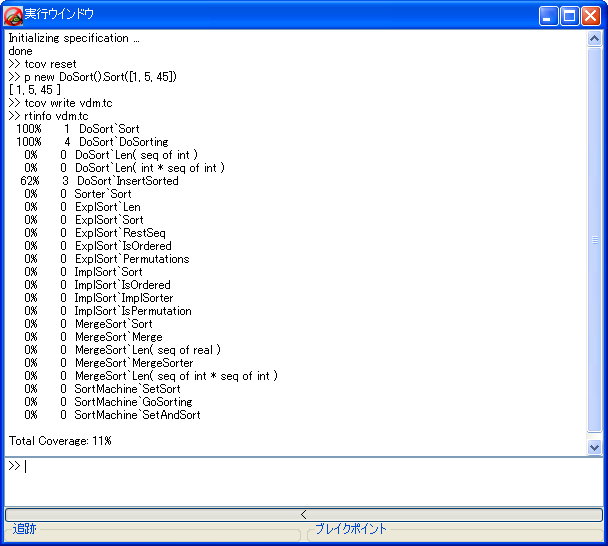
\includegraphics[width=12.5cm]{testCov-pp.png}
\caption{テストカバレッジ情報の収集}
\label{fig:guitcov}
\end{center}
\end{figure}


このプロセスは図~\ref{fig:guitcov}に記述されている。まず{\tt tcov reset}\index{tcov resetコマンド}をテストカバレッジ
ファイルをリセットするために発行するため、与えられた仕様のテスト情報には何も
載っていない。それから仕様と異なる物を評価するため\guicmd{print}コマンドを使う。それから、
\guicmd{tcov write}\index{tcov writeコマンド}で先ほど
の\guicmd{tcov reset}を発行してから生成されたテストカバレッジ情報
すべてを\texttt{vdm.tc}ファイルに保存する。最後に、コマンド\guicmd{rtinfo}\index{rtinfoコマンド} が
テストカバレッジファイルの情報を要約したテーブルを表示する。これが仕様のさまざまな関数や操作
のリストをひとつに構成し、それぞれテスト中に何回その関数/操作が呼び出され
ているかと、仕様の1度以上テストされた箇所のパーセンテージの注釈がつく。

\vdmslpp\ \Toolbox\ (\ifthenelse{\boolean{VDMsl}}{\texttt{vdmde}}{\texttt{vppde}})
のコマンドラインバージョンもテストカバレッジ情報の収集をサポートするため
同様の機能を有していることに注意してほしい。

\guicmd{tcov write} コマンドを使って\texttt{vdm.tc} ファイルにテストカバレッジ情報を書き込む前に、
実際のテストでは自然にもっとたくさんのテストを増やしていくものだ。本当に実際の
プロジェクトでは、一般的にこのプロセス全体を自動化するために小さなスクリプトファイル
を書くなどして全体的なテスト環境を構築したする。これもまた予測される結果に対する
実際の個々のテスト結果と比較できる(通常{\tt -O} オプションが使うのに必要である)。
付録~\ref{sec:testscript}にこのようなWindowsとUnixのスクリプトファイルの例が含まれている。

\subsection{清書機能}\label{subsec:pp}


\index{せいしょきのう@清書機能}
%\index{generating \LaTeX|see{pretty printing}}
%\index{latex@\LaTeX|see{pretty printing}}

清書機能は仕様を入力フォーマットから清書版に変更する。この
清書版は大体ドキュメント化の目的で使われる。
  
清書機能が動いているところを見るには、まず\guicmd{プロジェクトオプション} 画面の
\guicmd{清書}タブをクリックし、インデックスを生成するためにオプションをひとつ有効にし
(RTFフォーマットが使われていれば2つのうちどちらを使っても問題はない)、テストカバレッジの
色オプションも有効にする。たった今\Toolbox\ のワーキングディレクトリ に生成した{\tt vdm.tc}ファイルを
コピーしておく必要もある。インタープリタの\guicmd{入力} 画面から{\tt pwd}\index{pwdコマンド}を入力することで確定できる。

\guicmd{マネージャー}の\guicmd{プロジェクトビュー}で
\ifthenelse{\boolean{VDMsl}}{the {\tt sort-init.rtf} ファイル}{6つの {\tt .rtf} ファイルすべて} 
を選択し、(\guicmd{アクション})ツールバーの 
\raisebox{-1.0mm}{
\includegraphics[width=0.03\textwidth]{prettyprint.png}}
(\guicmd{清書}) ボタンを押す。\guicmd{ログウインドウ} に
\ifthenelse{\boolean{VDMsl}}{ファイル{\tt sort-init.rtf.rtf}}{
それぞれの選択された入力ファイルに対応する {\tt .rtf.rtf} ファイル}
が出来ているのがわかるはずだ。
\ifthenelse{\boolean{VDMsl}}{{\tt sort-init.rtf.rtf}}{{\tt dosort.rtf.rtf}}
ファイルでWordを起動してみる。
\vdmslpp\ のキーワードはすべて太字になっていることに注意してほしい。仕様のその他の部分は、
Wordの{\tt VDM\_COV}  と  {\tt VDM\_NCOV} 形式を使って書かれており、それぞれカバーされた部分とカバー
されていない部分に関連している。これらの形式の定義は変更することができ、ドキュメントに
カラープリンタを使うのであれば{\tt VDM\_NCOV} 形式の定義を変更する必要がある
(例\ カバーされていない部分はグレーを使う)

\ifthenelse{\boolean{VDMsl}}{{\tt sort-init.rtf.rtf}}{{\tt dosort.rtf.rtf}}
ファイルの最後に行ってみよう。{\tt VDM\_TC\_TABLE} 形式で書かれた
テキストがどのようにテストカバレッジを示す統計資料をあらわすテーブルに置き換わっているか
に注目。3つの欄が関数/操作名、テストカバレッジファイル内で呼ばれた回数、
それのカバレッジのパーセンテージの3つである。テーブルはこのようになる\footnote{前のセクションのインタープリタの
\guicmd{応答} 画面内で直接見られた情報の一部にとてもよく似ていることに注意。} 

\begin{center}
\begin{tabular}{|l|r|r|}\hline
\textbf{name}   & \textbf{\#calls} & \textbf{coverage} \\ \hline
DoSort          & 4     & 100\% \\
ExplSort        & 0     & 0\%\\
InsertSorted    & 3     & 62\%\\
IsOrdered       & 0     & 0\%\\
IsPermutation   & 0     & 0\%\\
Merge           & 0     & 0\%\\
MergeSort       & 0     & 0\%\\
Permutations    & 0     & 0\%\\
RestSeq         & 0     & 0\%\\
\textbf{total}  &       & 15\%\\\hline
\end{tabular} 
\end{center}


最後に、ファイルの最後にいって、Wordの\guicmd{挿入} プルダウンメニューから\guicmd{Index
and Tables ...}を選択する。
\ifthenelse{\boolean{VDMsl}}{{\tt sort-init.rtf.rtf}}{{\tt dosort.rtf.rtf}}
の定義の概要の見出しのためのレイアウトを希望するものに決めて\guicmd{Ok}ボタンを押すと
DMの定義のインデックスが自動的に生成される。

双方向の清書機構を\LaTeX\ に使用する際とはまったく違うが、このマニュアルの
リファレンスセクション(セクション~\ref{sec:testing}参照)で説明する。

\subsection{コード生成}
\index{C++コードせいせい@C++コード生成}
\index{コードせいせい@コード生成 |see {\\ C++コード生成, \\ Javaコード生成}}


\vdmslpp\ からC++へのコード生成のライセンス\index{ライセンス} を持っていれば、 
\raisebox{-1.0mm}{\includegraphics[width=0.03\textwidth]{cplusplus.png}}
(\guicmd{C++生成}) ボタンを押して自動的に仕様からC++のコードを生成することが出来る。
C++コード生成についての詳細は、
\ifthenelse{\boolean{VDMsl}}{\cite{CGMan-SCSK}}{\cite{CGManPP-SCSK}}を参照のこと。



\index{Javaコードせいせい@Javaコード生成}

同様に、\vdmslpp\ からJavaへのコード生成のライセンスを持っていれば、
\raisebox{-1.0mm}{\includegraphics[width=0.03\textwidth]{java.png}}
(\guicmd{Java生成}) ボタンを押すことで自動的に仕様からJavaのコードを生成することができる。
Javaコード生成の詳細については、\cite{CGJavaManPP-SCSK} を参照のこと。




\subsection{\protect\VDMTools\ API}

\VDMTools\ のすべての機能は、Corba APIを経由して外部プログラムにエクスポートすることができる。
APIの使い方についての詳細は\cite{APIMan-SCSK}を参照のこと。

%\subsubsection{Display of test coverage information in the GUI} \label{guirti}

%The tool \texttt{Test Coverage Tool} in the GUI can be used for
%displaying the collected test coverage information. The tool should be
%opened, the file for which test coverage information is wanted should
%be selected, and the button \texttt{Show Coverage} should be pressed.
%The specification file will be shown in the display window with the
%uncovered expressions and statements marked on the leading character
%with a red background (or underlined for B\&W displays).

\subsection{\protect\VDMTools の終了}


\Toolbox\ を終了させたいときは、メインウインドウの\guicmd{プロジェクト} メニューから\guicmd{終了} を選ぶ。
プロジェクトを保存せずに終了しようとすると、ダイアログが現れてプロジェクトを保存するかどうか聞いてくる。

これで\Toolbox\ の「ガイドツアー」は終了である。ツールの提供する機能がよりよく理解出来ていることと思う。
自身の\vdmslpp\ のモデルで\Toolbox\ を使い始められるようになっているはずだ。このマニュアルの残りの部分では、
特定の部分の特徴について詳細なリファレンスガイドとなっている。

\newpage
\section{\protect\VDMTools\ リファレンスマニュアル}\label{sec:ref}


このセクションは\Toolbox\ 内のツールそれぞれをカバーする数々のサブセクションで
構成されている。それぞれのツールはGUI、Emacs、コマンドラインの各インターフェースで
使用することができる。以下それぞれについて記述する。

\subsection{GUI全般}\label{sec:GUI}
\index{GUI}\index{GUI!スタート}


\Toolbox\ のGUIはウインドウズのプログラムから選択するか、Unix環境で{\tt \vdmgde}\index{vdmgdeコマンド} を
入力することで起動する。図~\ref{fig:startgui2}に示すGUIのメインウインドウが開く。

\begin{figure}[tbh]
\begin{center}
\includegraphics[width=11cm]{startgui-pp.png}
\caption{GUIスタートアップ画面}
\label{fig:startgui2}
\end{center}
\end{figure}


ウインドウのトップは6つのプルダウンメニューで構成されており、その下にはメニューと
同様のアクション を提供するボタン\footnote{ツールボックスの終了は\guicmd{プロジェクト} 
メニューからしかできない}から成る6つのツールバー
\footnote{\Toolbox\ を起動したときはツールバーは3つしか開いておらず、他の3つは
上部にアイコン化されて表示されている.} 
がある。ウインドウの下の
部分は現在のプロジェクトの状態についての情報や\Toolbox\ 内ツールのインターフェースを提供する
さまざまなサブウインドウを表示するのに使われる。以下のサブセクションでは、メニュー、
ツールバー、サブウインドウそれぞれについて機能別に記述する。

\subsubsection{プロジェクト・ハンドリング}\index{プロジェクト}
プロジェクトは\vdmslpp\ 形式の仕様のファイルを集めたもので構成される。
プロジェクトは保存されディスクから読み込むことが出来るが、これは\Toolbox\ に
個々のファイルを毎度毎度使いたいときに保存する設定をする必要がないことを意味する:
ただ適切なプロジェクトファイルを開けばよいだけなのだ。プロジェクトはGUIでのみ利用できる。

\guicmd{マネージャー}\index{マネージャー}は、\guicmd{ウインドウ} メニューから適切なものを
選択するかまたは\guicmd{ウインドウ} 
ツールバーの\raisebox{-1.0mm}{\includegraphics[width=0.03\textwidth]{browser.png}}ボタンを
押下することで起動/終了するが、現在のプロジェクトの状態を表示するだけ
でなく、操作しようとするプロジェクトファイルのサブセットに対し適用しようとするさまざまな\Toolbox\ の
操作を選ぶ場所でもある。\guicmd{プロジェクトビュー} と
\ifthenelse{\boolean{VDMsl}}{\guicmd{モジュールビュー}}{\guicmd{クラスビュー}}
の2つで構成される。

\guicmd{プロジェクトビュー} はプロジェクトのファイル構成(構文チェック済みのファイルのみ)と各々のファイルで
宣言されている
\ifthenelse{\boolean{VDMsl}}{モジュール}{クラス} の内容をツリー構造で表示する。
図\ref{fig:projectView}にそれを示す。

\begin{figure}[tbh]
\begin{center}
\mbox{}
\includegraphics[width=9cm]{projectView-pp.png}
\caption{プロジェクトビュー}
\label{fig:projectView}
\end{center}
\end{figure}



\guicmd{クラスビュー} は \guicmd{VDMビュー} と\guicmd{Javaビュー}で構成される。



\vdmslpp\ のファイルが構文チェックを無事パスすると、それらのファイルで定義されている
\ifthenelse{\boolean{VDMsl}}{モジュール}{クラス} の
名前が\vdmModView\ にリスト表示される。このビューはプロジェクトでの
\ifthenelse{\boolean{VDMsl}}{モジュール}{クラス} それぞれの状態を記号
\raisebox{-0.7mm}{\includegraphics[width=0.03\textwidth]{syntaxcheckdone.png}},
\raisebox{-1.0mm}{\includegraphics[width=0.03\textwidth]{typecheckdone.png}},
\raisebox{-1.0mm}{\includegraphics[width=0.03\textwidth]{cplusplusdone.png}},
\raisebox{-1.0mm}{\includegraphics[width=0.03\textwidth]{javadone.png}},
\raisebox{-1.0mm}{\includegraphics[width=0.03\textwidth]{prettyprintdone.png}}
で各々適切な欄にこれらは、当該\ifthenelse{\boolean{VDMsl}}{モジュール}{クラス} が
正常に構文チェック済み(syntax checked)、型チェック済み(type checked)、
C++コードを生成済み(translated to C++)、
\ifthenelse{\boolean{VDMsl}}{}{Javaコードを生成済み(translated to Java)、} 清書済み(pretty printed)
なのを示すが、似たような印で各記号に赤線が入ったもの
(%
\raisebox{-0.7mm}{\includegraphics[width=0.03\textwidth]{syntaxcheckerror.png}},
\raisebox{-1.0mm}{\includegraphics[width=0.03\textwidth]{typecheckerror.png}},
\raisebox{-1.0mm}{\includegraphics[width=0.03\textwidth]{cpluspluserror.png}},
\raisebox{-1.0mm}{\includegraphics[width=0.03\textwidth]{javaerror.png}},
\raisebox{-1.0mm}{\includegraphics[width=0.03\textwidth]{prettyprinterror.png}})
は個々の処理が失敗したことを示す。空欄だった場合は、まだ個々の処理が実行されて
いないことを示す。プロジェクト中のファイルのひとつがこのシステム上で修正されると、\guicmd{構文} 欄
に現在の\Toolbox\ でのファイルのバージョンとファイルシステムでのバージョンに不整合が起こっ
ていることを示す記号が表示される。そのファイルは他の処理に進む前に再度構文チェックを行うべきである。



\guicmd{Javaビュー} は\guicmd{VDMビュー} と似ているがJavaファイルで定義されたクラスの状態と名前を表示するところが
異なる(しつこいようだが構文チェックが成功していないと表示されない)。クラスが正しく構文チェック/型チェックを
通ったかを示す記号
\raisebox{-0.7mm}{\includegraphics[width=0.03\textwidth]{syntaxcheckdone.png}},
\raisebox{-0.7mm}{\includegraphics[width=0.03\textwidth]{syntaxcheckerror.png}},
\raisebox{-1.0mm}{\includegraphics[width=0.03\textwidth]{typecheckdone.png}},
\raisebox{-1.0mm}{\includegraphics[width=0.03\textwidth]{typecheckerror.png}}
が再度該当する欄に表示される。3つ目の欄にはクラスがそれぞれJavaから \vdmslpp\ へ正しく変換されたかどうか(
\raisebox{-1.0mm}{\includegraphics[width=0.03\textwidth]{java2vdmdone.png}},
\raisebox{-1.0mm}{\includegraphics[width=0.03\textwidth]{java2vdmerror.png}})
が表記される。もう一度言うが空欄はまだ個々の処理が一度も実行されていないことを意味する。
プロジェクト中のファイルのひとつがこのシステム上で修正されると、\guicmd{構文チェック} 欄に 
\raisebox{-0.7mm}{\includegraphics[width=0.03\textwidth]{syntaxcheckmodified.png}}マークが表示され、
現在の\Toolbox\ でのファイルのバージョンとファイルシステムでのバージョンに不整合が起こっていることを示す。
そのファイルは他の処理に進む前に再度構文チェックを行うべきである。



プロジェクトを開く/保存する、プロジェクトへのファイルの追加と削除、新規プロジェクトの作成などを
含むプロジェクト操作のためのさまざまな処理が\guicmd{プロジェクト}メニューとそれに相当する\guicmd{プロジェクト}
ツールバーから利用できる。これを図~\ref{fig:projectMenuToolbar}に示す。

\begin{figure}[tbh]
\begin{center}
\mbox{}
\includegraphics[width=11cm]{projectMenuToolbar-pp.png}
\caption{プロジェクトメニューとプロジェクトツールバー}
\label{fig:projectMenuToolbar}
\end{center}
\end{figure}


同じメニュー/ツールバーを使って、\Toolbox\ の環境に関係するオプション設定、
\Toolbox\ 中のさまざまなツールのオプション設定、\Toolbox\ の終了(メニューからのみ可能)
をすることができる。以下で利用できる処理について詳しく述べる。

\begin{description}


\item[\guicmd{新規プロジェクト} (\hspace{-1.8mm}
\raisebox{-0.8mm}{\includegraphics[width=0.03\textwidth]{projectnew.png}}):]
  新しいプロジェクト上で作業を始めたいときに選ぶ項目

\item[\guicmd{プロジェクトを開く} (\hspace{-1.2mm}
\raisebox{-0.8mm}{\includegraphics[width=0.03\textwidth]{load.png}}\hspace{.6mm}):]
  すでに存在するプロジェクトを開きたいときに選ぶ項目。ファイルブラウザが表示され希望する
  プロジェクトファイルを選択することができる。これがロードされると\Toolbox\ はプロジェクト中の
  すべてのファイルに自動的に構文チェックをかける。

\item[\guicmd{保存} (\hspace{-1.8mm}
\raisebox{-0.8mm}{\includegraphics[width=0.03\textwidth]{projectsave.png}}):]
  プロジェクトの設定を変えてそれを保存したいときに使用する項目

\item[\guicmd{別名で保存} (\hspace{-1.5mm}
\raisebox{-0.8mm}{\includegraphics[width=0.03\textwidth]{projectsaveas.png}}):]
  現在の構成を別な名前で保存したい場合に使う。ファイルブラウザが表示され新しい
  プロジェクトを保存する場所を好きに設定できる。また名前も好きなものに出来る。

\item[\guicmd{ファイルを追加} (\hspace{-1.5mm}
\raisebox{-0.8mm}{\includegraphics[width=0.03\textwidth]{plus.png}}):] 
  ツールボックス上の現在のプロジェクトにファイルを追加するときに使う。
  図~\ref{fig:addFiles} に示したようなウインドウが表示され、追加したいファイルを選択することができる。

\item[\guicmd{ファイルを削除} (\hspace{-1.5mm}
 \raisebox{-0.8mm}{\includegraphics[width=0.03\textwidth]{minus.png}}):]
 プロジェクトからファイルを削除したいときに使う。削除の確認ダイアログが表示される。

\item[\guicmd{プロジェクトオプション} (\hspace{-1.5mm}
\raisebox{-0.8mm}{\includegraphics[width=0.03\textwidth]{projectoptions.png}}):].
  \begin{itemize}
    \item \guicmd{実行} (セクション ~\ref{sec:interpreter}参照);
    \item \guicmd{型チェック}  (セクション~\ref{sec:tc}参照);
    \item \guicmd{清書}  (セクション~\ref{sec:pp}参照);
    \item \guicmd{C++コード生成} (セクション~\ref{sec:cg}参照)

    \item \guicmd{Javaコード生成}  (セクション~\ref{sec:cgjava}参照);
    \item \guicmd{Java からVDM++生成}  (~\cite{Java2VDMMan-SCSK}参照). 
  \end{itemize}

\item[\guicmd{ツールオプション} (\hspace{-1.5mm}
\raisebox{-0.8mm}{\includegraphics[width=0.03\textwidth]{tooloptions.png}}):].
  \guicmd{ツールオプション} ウインドウを開く。\Toolbox\ のインターフェースオプションの
  設定ができる。これらのオプションについては付録~\ref{sec:set_env}を参照のこと。

\item[\guicmd{最近使ったプロジェクト}:]
  PCで最近使ったプロジェクトのリストを開く。

\item[\guicmd{終了}:]
  \Toolbox\ を終了する。プロジェクトを保存していない場合は、\Toolbox\ が
  保存するかどうかを聞いてくる。ツールバーからは使えないことに注意。

\end{description}

\subsubsection{仕様の操作}


 \Toolbox\ は仕様に適用させうる広範囲な機能を提供している:構文チェック、
型チェック、証明課題の生成、
C++\ifthenelse{\boolean{VDMsl}}{}{/Java} のコード生成、
\ifthenelse{\boolean{VDMsl}}{}{Javaから \vdmslpp の生成、;} 
清書など。これらはアクションメニューまたはそれに
相当するアクションツールバーから起動することが出来る。図~\ref{fig:actionsMenuToolbar}にこれを示す。

\begin{figure}[tbh]
\begin{center}
\mbox{}
\includegraphics[width=11cm]{actionsMenuToolbar-pp.png}
\caption{アクションメニューとツールバー}
\label{fig:actionsMenuToolbar}
\end{center}
\end{figure}


それぞれのアクションはマネージャで現在選択中のファイル・
\ifthenelse{\boolean{VDMsl}}{モジュール}{クラス} 各々に適用される。
アクションはある程度まで相互依存しているため、そのうちのいくらかは選択された
\ifthenelse{\boolean{VDMsl}}{モジュール}{クラス}  が
求められ適用する機能を可能にする状態の時にのみ実行される。例えば、型チェック機能と
清書の機能は
\ifthenelse{\boolean{VDMsl}}{モジュール}{クラス} が構文チェック機能をパスしてから適用できる。

さまざまなアクションが下記に示すセクションで詳細に記述される。

\begin{description}


\item[\guicmd{構文チェック} (\hspace{-1.8mm}
\raisebox{-0.8mm}{\includegraphics[width=0.03\textwidth]{syntaxcheck.png}}):] セクション~\ref{sec:parser}参照 

\item[\guicmd{型チェック} (\hspace{-1.8mm}
\raisebox{-0.8mm}{\includegraphics[width=0.03\textwidth]{typecheck.png}}):] セクション~\ref{sec:tc}参照 

\item[\guicmd{証明課題生成} (\hspace{-1.8mm}
\raisebox{-0.8mm}{\includegraphics[width=0.03\textwidth]{integritycheck.png}}):] セクション~\ref{sec:pog} 参照

\item[\guicmd{C++コード生成} (\hspace{-1.8mm}
\raisebox{-0.8mm}{\includegraphics[width=0.03\textwidth]{cplusplus.png}}):] セクション~\ref{sec:cg}参照 

\item[\guicmd{Javaコード生成} (\hspace{-1.8mm}
\raisebox{-0.8mm}{\includegraphics[width=0.03\textwidth]{java.png}}):] セクション~\ref{sec:cgjava}参照

\item[\guicmd{清書} (\hspace{-1.8mm}
\raisebox{-0.8mm}{\includegraphics[width=0.03\textwidth]{prettyprint.png}}):] セクション~\ref{sec:pp}参照

\item[\guicmd{JavaからVDM生成} (\hspace{-1.8mm}
\raisebox{-0.8mm}{\includegraphics[width=0.03\textwidth]{java2vdm.png}}):] ~\cite{Java2VDMMan-SCSK}参照 


\end{description}

\subsubsection{ログウインドウ、エラーリストウインドウ、ソースウインドウ}


\guicmd{ログウインドウ} は\Toolbox\ からのメッセージを表示するが、これには上で記述
した動きを適用したときの成功・失敗の報告メッセージを含む。すでに開いていない限り、
新しいメッセージを表示するときに自動的に開く。代わりに\guicmd{ウインドウ} ツール
バーで \raisebox{-0.8mm}{\includegraphics[width=0.03\textwidth]{log.png}}
ボタンを押すか\guicmd{ウインドウ} メニューで相当する項目を選ぶことで手動でウインドウ
を開いたり閉じたりすることも出来る。

%   The \guicmd{Log Window} has three icons:
%   \begin{list}{}{}
%   \item[\includegraphics{clearBig}] This erases the content of the
%     log window.
%   \item[\resizebox{1cm}{!}{\includegraphics{print}}] This prints
%     the content of the frame to your printer. (Not available on the
%     Windows platform).
%   \item[\resizebox{1cm}{!}{\includegraphics{pipe}}] This pipes the
%     content of the buffer. When you select this icon a window pops up
%     and asks for a command to do the pipe command. (Not available on
%     the Windows platform).
%   \end{list}

\guicmd{エラー一覧} はアクション実行中に\Toolbox\ によって発見されたエラーを報告する。
図~\ref{fig:error2}に示すとおり2つの画面から構成される。上のほうの画面はエラーやワーニングの
起こった箇所(ファイル名、行数、欄番号)のリストを示し、一方下の画面では
選択中のエラーの詳細な説明が表示される。構文チェック中や型チェック中に
生じるさまざまなエラーの形式は、セクション~\ref{subsub:synerr} と~\ref{subsub:tcerr} に
それぞれ記述されている。最初は、自動的にリストの先頭のエラーが選択されている。
エラーリストの左にある {\fbox{\tt >}} or \fbox{{\tt <}} ボタンを押すことでエラーリスト内の
次・前へ移動できる。代わりに\guicmd{エラー一覧}の上の画面にあるエラー通知を示す印を直接選択
しても任意のエラーへ動かすことができる。

\begin{figure}[tbh]
\begin{center}
\includegraphics[width=\textwidth]{errorList-pp.png}
\caption{エラー一覧}
\label{fig:error2}
\end{center}
\end{figure}


\guicmd{エラー一覧} はすでに開いていない限り新しいエラーが見つかると自動的に開く。
代わりに \guicmd{ウインドウ} ツールバーで 
\raisebox{-0.8mm}{\includegraphics[width=0.03\textwidth]{error.png}}ボタンを押すか
\guicmd{ウインドウ} メニューで相当する項目を選ぶことで手動でウインドウを開いたり
閉じたりすることも出来る。

\guicmd{ソースウインドウ} もまたすでに開いていない限り新しいエラーが見つかると自動的に開く。
現在選択中のエラーが発見された元の仕様の一部を表示し、実際のエラーの位置は
ウインドウズのカーソルでマークされる。図~\ref{fig:error2}に記述された\guicmd{エラー一覧} に
相当する\guicmd{ソースウインドウ} を図~\ref{fig:source2}に示す。

\begin{figure}[tbh]
\begin{center}
\caption{ソースウインドウ}
\label{fig:source2}
\end{center}
\end{figure}


多くのソースファイルが\guicmd{ソースウインドウ}に表示されているが、内容が表示されている
のはそのうち1つだけである。違うソースファイルを見たければ、\guicmd{ソースウインドウ}の上部に
あるファイルに相当するタブを選択することで表示が変わる。新しいソースファイルを
足すには、\guicmd{マネージャー}で手動でファイル名(またはファイルに含まれる
\ifthenelse{\boolean{VDMsl}}{モジュール}{クラス} のひとつ)を
ダブルクリックする。ソースファイルは\guicmd{ファイル} ツールバーの 
\raisebox{-0.8mm}{\includegraphics[width=0.03\textwidth]{fileclose.png}}
(\guicmd{ソースウインドウから選択されたファイルを閉じる}) ボタン
または 
\raisebox{-0.8mm}{\includegraphics[width=0.03\textwidth]{filecloseall.png}}
(\guicmd{ソースウインドウのすべてのファイルを閉じる}) ボタンを押すと画面上から消える。 
\raisebox{-0.8mm}{\includegraphics[width=0.03\textwidth]{fileclose.png}})ボタンは
現在表示中のファイルを閉じ、
\raisebox{-0.8mm}{\includegraphics[width=0.03\textwidth]{filecloseall.png}})ボタンは
すべてのファイルを閉じる。

\guicmd{ソースウインドウ} は\guicmd{ウインドウ} ツールバーの
\raisebox{-0.8mm}{\includegraphics[width=0.03\textwidth]{source.png}}ボタンを
押すか\guicmd{ウインドウ} メニューから同様の項目を選択することで開いたり閉じたり出来る。

\subsubsection{ファイルの編集}


\Toolbox\ を終了させずにエラーを修正するために、好みのエディタ(付録~\ref{sec:set_env}参照)を
作業中のプロジェクトのファイルから直接起動することができる:単純に編集したいファイルを
\guicmd{Manager} で選択し、\guicmd{プロジェクト}ツールバーの\guicmd{外部エディタ}
\index{がいぶエディタ@外部エディタ} ボタン(%
\raisebox{-0.8mm}{\includegraphics[width=0.03\textwidth]{externaleditor.png}})を押す。
この方法で\guicmd{外部エディタ}を起動するときに複数のファイルが選択した場合、ひとつの
\guicmd{外部エディタ}で選択したファイルそれぞれを表示する。

\Toolbox\ はエディタで保存した変更を自動的に登録する。しかし編集されたファイルの
バージョンは自動的に更新されることはないので、ソースファイルを編集したら他のツールを使う前に
必ず構文チェック機能を再度走らせれば、\Toolbox\ にも変更が反映される。

% \subsubsection{Tracking dependencies}

% The \guicmd{References} window displays the dependencies between
% classes, that is the classes which use the selected class and the
% classes which the selected class uses~(a class {\em uses\/} another
% class if it has references to objects of that class, for example
% through its instance variables or operation calls). It can be opened
% by pressing the  
% \raisebox{-0.8mm}{\includegraphics[width=0.03\textwidth]{references}}
% button on the \guicmd{Window Operations} toolbar or by selecting the
% corresponding item from the \guicmd{Windows} menu, and closed by
% pressing the \guicmd{Ok} in the bottom right-hand corner of the window
% itself. %\fbox{{\bf needs completing! -- RM}}.
% This feature is not yet implemented. 

\subsubsection{インタープリタを使う}


インタープリタを使って式と文のデバッグ、評価ができる。\guicmd{実行ウインドウ}
はインタープリタへのインターフェースを提供するが、(\guicmd{ウインドウ})ツールバーの 
\raisebox{-1.0mm}{\includegraphics[width=0.03\textwidth]{interpreter.png}}  
(\guicmd{実行}) ボタンを押すと開く。また\guicmd{実行} メニューおよびツールバーは
インタープリタでできるあらゆる処理を提供する。詳細はセクション~\ref{sec:interpreter}で記述する。

\subsubsection{オンラインヘルプ}
\index{ヘルプ}
% 
% %%%%% This next paragraph should be reinserted when help window is
% %%%%% implemented -- RM
%
% At any time when you are using the \Toolbox\ you can press the ``{\tt
%   F1}'' button and a help window~(as shown in
% Figure~\ref{fig:guihelp}) will appear with on-line help for the
% graphical user interface. The part of the help text that is shown at
% the top of the help window is related to the particular part of the
% \Toolbox\ window in which the cursor is placed. The help text is
% organised in a hypertext format so it is possible to follow links from
% one part of the help text to another.

% The help window can also be accessed by pressing the  
% \raisebox{-0.8mm}{\includegraphics[width=0.03\textwidth]{help}}
% button on the \guicmd{Help} toolbar or by selecting the corresponding
% item from the \guicmd{Help} menu. 


\Toolbox\ のオンラインヘルプと一般的なインターフェースは\guicmd{ヘルプ} ツールバーや\guicmd{ヘルプ} メニューから
アクセスできる。最近では以下に示す限られたものだけが利用可能である。

\begin{description}

 \item[\guicmd{ツールについて} (\hspace{-1.8mm}
\raisebox{-0.8mm}{\includegraphics[width=0.03\textwidth]{help.png}}):]
  \Toolbox\ のバージョン番号を表示する

 \item[\guicmd{Qtについて}  (\hspace{-1.8mm}
\raisebox{-0.8mm}{\includegraphics[width=0.03\textwidth]{qt.png}}):]
  Qt(\Toolbox\ のインターフェースが利用している、C++のマルチプラットフォーム
  GUIツールキット)へのリファレンス情報を表示する

% \item[\guicmd{What's This?} (\hspace{-1.8mm}
%\raisebox{-0.8mm}{\includegraphics[width=0.03\textwidth]{whatsthis}}):]  
%  これを選択してから\Toolbox\ の一部の上でマウスの左ボタンをクリックすると、
%  その項目についての記述が表示される(現在は一部のみ実装されている)
\end{description}


\subsection{コマンドラインインターフェース全般}\label{subsec:maincommand}
\index{コマンドラインインターフェース}\index{コマンドラインインターフェース!かいし@開始}


コマンドラインインターフェースはプロンプトから以下のように入力 することで起動する。
\footnote{実行可能な{\tt \vdmde}コマンドがサーチパスに必ずあるか、フルパス指定をしなくてはならない}:

{\tt \vdmde\ [-o scriptfile] [-q] [specfiles]}

コマンドラインから{\tt \vdmde} がファイル名(\vdmslpp\ の仕様を
含んでいなければならない)で起動されると、ツールはコマンドモードに入り指定された
ファイルの構文チェックを始める。
{\tt -o scriptfile}をつけると、指定された仕様を読み込んだ後に、スクリプトファイルに記述
されたスクリプトを実行する。{\tt -q}オプションをつけると、すべての処理が終了した時点で、
{\tt \vdmde} は終了する。

ユーザーは\Toolbox\ が提供するたくさんのコマンドをプロンプトからタイプすることで、
仕様の操作、実行、デバッグができる。下記で与えられたコマンドは{\tt \vdmde}によってサポートされている。
丸カッコ内の省略形はコマンドの短縮形である。

多くのコマンドが、仕様の初期化前には使用できない。({\cmd init}コマンドについては、
セクション~\ref{sec:interpreter}を参照)これらのコマンドには({\tt *})マークがついている。

種々の構成要素の名前を表示するのに、多くのコマンドが使われる。
\ifthenelse{\boolean{VDMsl}}{\textbf{modules},}{\textbf{classes},} 
\textbf{functions}, \textbf{operations}, 
\ifthenelse{\boolean{VDMsl}}{\textbf{states}}{\textbf{instvars}},
\textbf{types}, \textbf{values}
である。\textbf{info} または\textbf{help}を使って\Toolbox\ のコマンドの
ヘルプが得られる。
頻繁に使われるコマンドのシーケンスはスクリプトファイルに集められ、 \textbf{script} コマンドを使って
実行することができる。一般的なOSのシステムコールは\textbf{system} コマンドで発行することができる。
\textbf{dir}コマンドはツールボックスの検索パスにディレクトリを足すときに使う。\textbf{pwd} コマンドは現在の
ワーキングディレクトリを表示する。最後に\textbf{quit}または\textbf{cquit}コマンドでコマンドライン入力の
\Toolbox\ を終了することが出来る。下記でこれらコマンドについて記述する。

\begin{description}


\item[*classes] \index{classesコマンド}\mbox{} \\
  定義済みのクラス名とその状態を表示


\item[*functions]  \ifthenelse{\boolean{VDMpp}}{{\tt class}}{}\index{functionsコマンド}\mbox{}\\ 
  \ifthenelse{\boolean{VDMsl}}{現在のモジュール}{クラス{\tt class}}で定義される関数名を表示する。
  事前条件、事後条件、関数の不変条件は仕様がそれを含む場合自動的に作成される

\item[*operations] {\tt class}\index{operationsコマンド}\mbox{}\\
  与えられたクラス名で定義される操作名を表示する


\item[*instvars] {\tt class}\index{instvarsコマンド}\mbox{}\\
  与えられたclass名で定義されるインスタンス変数名を表示する


\item[*types] \ifthenelse{\boolean{VDMpp}}{{\tt class}}{}\index{typesコマンド}\mbox{}\\ 
  \ifthenelse{\boolean{VDMsl}}{現在のモジュールで}{与えられたクラス名で}
  定義済みの型名を表示する

\item[*values] \ifthenelse{\boolean{VDMpp}}{{\tt class}}{}\index{valuesコマンド}\mbox{}\\ 
  \ifthenelse{\boolean{VDMsl}}{現在のモジュールで}{与えられたクラス名で}
  定義される値の名前を表示する

\item[help \mbox{[{\tt command}]}] \index{helpコマンド}\mbox{}\\
  このセクションで使われているような、すべての利用可能なコマンドを説明する
  オンラインヘルプと同じスタイル。引数なしだと利用可能なコマンドすべてのリストを
  表示する。そうでない場合は引数で与えられた{\tt コマンド}の説明となる。

\item[info \mbox{[{\tt command}]}] \index{infoコマンド}\mbox{}\\
  {\tt help}と同じ。

\item[script {\tt file}] \index{scriptコマンド}\mbox{}\\
  {\tt file}からスクリプトを読み込み、実行する。スクリプトは\vdmslpp\ コマンドの羅列である。
  これらはコマンドラインインターフェースであればこのセクションや他のセクションで記述
  されたどのコマンドも使用できる。スクリプトの実行が終わると、コントロールは\Toolbox\ に戻る

\item[system (sys) {\tt command}]\index{systemコマンド}\mbox{}\\
  シェルコマンドを実行する

\item[dir \mbox{[{\tt path ...}]}] \index{dirコマンド}\mbox{}\\
  アクティブなディレクトリのリストにディレクトリを追加する。これらのディレクトリは
  仕様のファイルの場所を探すとき自動的にサーチされる。
  このコマンドを引数なしで実行するとアクティブなディレクトリのリストが画面に
  表示される。ディレクトリは表示された順にサーチされる。

\item[pwd] \index{pwdコマンド} \mbox{}\\
  現在のワーキングディレクトリを表示する。例えば、プロジェクトファイルがあれば
  作業中のプロジェクトファイルのある場所である。すべての場合、vdm.tcファイルのある
  場所であり、コード生成で生成されたファイル\ifthenelse{\boolean{VDMpp}}{やRose-VDM++リンク}{} 
  が書き込みをするところとなる。

\item[encode \mbox{[{\tt encoding}]}] \index{encodeコマンド}\mbox{}\\
  仕様が書かれている文書の文字コードを設定する。

\item[cquit] \index{cquitコマンド} \mbox{}\\
  確認の質問なしでデバッガを終了する。バッチジョブでデバッガを
  使うときに利用するとよい

\item[quit (q)] \index{quitコマンド}\mbox{}\\
  {\tt cquit}と同じ
%\Toolbox\ の終了。確認の質問を聞いてくる\\

\end{description}

\subsubsection{ファイルの初期化}\index{コマンドラインインターフェース!ファイルのしょきか@ファイルの初期化}


コマンドラインインターフェースでは、「ファイルの初期化」をすることができる。
これらのコマンドは\Toolbox\ をコマンドラインで起動すると自動的に実行される。

初期化ファイルは{\tt .\vdmde ファイル}\index{.\vdmde ファイル}で指定され、
引数としてファイルを指定するためには
\Toolbox\ が起動するディレクトリか仕様のファイルのあるディレクトリと同じ
ディレクトリになくてはならない。

\newpage
\subsection{構文チェック機能}\label{sec:parser}


構文チェック機能は作成した仕様が言語定義であたえられている構文に沿うもので
あるかどうかチェックする。このシステムのほかのツールは仕様が構文的に正しい
前提で動くため、仕様は\Toolbox\ のほかのツールを適用する前に構文チェックを行い、
構文エラーのない状態にしておく必要がある。
\ifthenelse{\boolean{VDMsl}}{{\bf 元ファイルを修正した場合は、他のツールが
修正に気づく前に構文チェックを再度しておかなければ成らないことに注意すること。}}{}

構文チェック機能はGUI、コマンドライン、Emacsのいずれのインターフェースを使っても使用することができる。

構文チェック機能の狙いは仕様の構文エラーを出来るだけ多く同時にレポート
することである。このため、構文チェック機能は最新のリカバリー機構を使用しているが、
これにより構文エラーを見過ごしてしまう前に捕捉し復旧することや、すぐ次に
生じる仕様の構文エラーを報告することができる。仕様のある記号を
無視したり足りない記号を想定したりすることでこれを可能にする。
エラーメッセージは、仕様のエラーが起こった箇所で何が期待されていたかということや
チェッカーが実行し続けるためには何が無視されるべきで何が想定されるのかということに
ついての情報もあたえてくれる。最初は、何が想定/無視されるのかということに集中する
ことによってエラーメッセージを理解するのが最も簡単である。なぜならこの構文チェック機能に
よる推測は実際のエラーに近いものであることが多いからだ。

\subsubsection{GUI}


構文チェック機能をGUIで起動するには、チェックしたいファイルまたは
\ifthenelse{\boolean{VDMsl}}{モジュール}{クラス} (複数選択可能)
\footnote{
%--------------------------footnote inserted-----------
  \vdmModView\ で
  \ifthenelse{\boolean{VDMsl}}{モジュール}{クラス} を選択すると、構文チェック機能は実際には選択した
  \ifthenelse{\boolean{VDMsl}}{モジュール}{クラス} の含まれる
 ファイル一式に適用される−\Toolbox\ はどのファイルが編集されたかということしか知らない。
 これはもし特定のファイルが複数の
  \ifthenelse{\boolean{VDMsl}}{モジュール}{クラス} 定義を含んでいて、そのうちのいくつかだけを
  選択していた場合には、暗黙のうちに同じファイルの他
  \ifthenelse{\boolean{VDMsl}}{モジュール}{クラス} が処理に含まれる。
%--------------------------footnote inserted end-----------
}
を\guicmd{マネージャー} の\guicmd{プロジェクトビュー} または\vdmModView\ で選択して、
(\guicmd{アクション})ツールバーの \raisebox{-0.7mm}{\includegraphics[width=0.03\textwidth]{syntaxcheck.png}}  
(\guicmd{構文チェック})ボタンを押す。
\guicmd{ログウインドウ} が(開いていなければ)自動的に開き選択したファイルやクラスそれぞれのチェックの
進行状況についての情報を順番に表示する。構文エラー\index{こうぶんエラー@構文エラー}が発見されると、
\guicmd{エラー一覧}\index{エラーリスト} と\guicmd{ソースウインドウ} が自動的に起動する。

\subsubsection{構文エラーのフォーマット} \label{subsub:synerr}


仕様の構文エラーが見つかると、構文チェック機能\index{こうぶんエラー@構文エラー!フォーマット} は
\guicmd{エラー一覧}に以下のような情報を表示する。

\begin{enumerate}


\item
 構文エラーの箇所にどんな記号が(足りないことが)\textbf{想定される(expected)}か

\item
  構文エラーから復旧するにはどうすればよいか。記号を\textbf{挿入}するか、
  記号を\textbf{無視}するか、違う記号に\textbf{置き換える}かなど。仕様のファイル自体は
  この処理によって何も変わらない(構文チェック機能内でのみ実行される変化であり、
  これがさまざまな構文エラーを捕捉することを可能にしている)

\end{enumerate}

記号は3つの形式の混合で表示される:

\begin{itemize}

\item
     シングルクォート内に表示~e.g.\ {\tt `functions'}.

\item
  メタシンボルの表示~e.g.\ \verb!<end of file>!, 「ファイルの最後」の意味

\item
  似たようなトークン群をシングルトークンとして表示~e.g.\ 
  \verb!<<type>>!, 構文上のユニット {\tt type} (定義は
  \ifthenelse{\boolean{VDMsl}}{\cite{UMLMan-SCSK}}{\cite{LangManPP-SCSK}}) 予想される記号のリストを
  短くするためにこれがなされる
\end{itemize}

\subsubsection{コマンドラインインターフェース}\label{subsec:parcom}
\index{コマンドラインインターフェース!こうぶんチェッカー@構文チェック機能}

コマンドラインから構文チェック機能を起動するコマンドの構文は:

{\tt \vdmde\ -p [-w] [-R testcoverage] specfile(s) ...}

\vspace{0.5cm}

\noindent

{\tt -p} オプションをけると、{\tt \vdmde}コマンドはそれぞれ
\ifthenelse{\boolean{VDMsl}}{1つ以上のモジュール、またはフラットな仕様の一部}{1つ以上のクラス}
を含むたくさんのファイルをチェックする。
エラーは{\aaa stderr}で報告される。

その他の追加オプションは、

\begin{description}

\item[{\tt -w}]
   \vdmslpp\ のRTFファイルの一部をASCIIに書き出す。ASCIIのファイル名は
  RTFのファイル名に拡張子{\tt .txt}がつく。例){\tt sort.rtf}は{\tt sort.rtf.txt}となる

  このオプションはテスト環境で仕様の解析時間を減らすためによく使われる。
  RTFファイルの文書の部分が大きいと、ファイル全体を解析しなければならないため
  とても遅くなる。例えば、図はファイルの文書部分をとても大きくしてしまう傾向がある。

\item[{\tt -R}]
   \vdmslpp\ 仕様のテスト中違う構成要素がどれだけ実行されたかを記録するのに
  使われるテストカバレッジファイルを生成する。(ファイル名は引数
  {\tt testcoverage}で指定できる)現在のバージョンでは、このテストカバレッジ
  ファイルは{\tt vdm.tc}という名前でなくてはならない(清書機能が動くため)。
  例についてはセクション~\ref{vdmtc} を参照。

\item[{\tt -W code}] 仕様文書の文字コードを{\tt code}に設定する
\end{description}

\subsubsection{Emacsインターフェース}


Emacsインターフェースでは、すべてのコマンドをプロンプトから入力する。
構文チェックは\textbf{read}コマンドで行われ、構文エラーを詳しく見るには
\textbf{first}, \textbf{last}, \textbf{next}, \textbf{previous} コマンドが使われる。

\begin{description}

\item[read (r) {\tt file(s)}] \index{readコマンド}\mbox{}\\
  {\tt file(s)}から仕様の構文チェックを行う。
  \ifthenelse{\boolean{VDMsl}}
    {
      {\tt file(s)}はモジュール定義または関数、値、操作、型、場合によっては状態の定義を
      含まなくてはならない。
    }%
    {
      {\tt file(s)}は関数、値、型、インスタンス変数などを含むクラスの定義を含まなくてはならない。
    }

  それぞれのファイルの内容は全体として扱われる。これはもし構文エラーが
  起こっても、そのファイルの\vdmslpp\ での構成要素は何も含まれないということを意味する。
  またこれはもしそのファイルが複数の
  \ifthenelse{\boolean{VDMsl}}{モジュール}{クラス} を含んでいた場合も含む
  (\ifthenelse{\boolean{VDMsl}}{モジュール}{クラス}  には何も含まれない)。
  ファイルが構文チェックをパスし、構文チェック済みのファイルですでに定義された
  \ifthenelse{\boolean{VDMsl}}{モジュール}{クラス} が再定義
  されたならば、ワーニングが発生する。

\item[first (f)] \index{firstコマンド}\mbox{}\\
  構文チェック機能、型チェック機能、コード生成、清書機能
  からなど最初に記録されたエラーまたはワーニングメッセージを表示する。

\item[last] \index{lastコマンド}\mbox{}\\
  構文チェック機能、型チェック機能、コード生成、清書機能
  などから最後に記録されたエラーまたはワーニングメッセージを表示する。

\item[next (n) \index{nextコマンド}]\mbox{}\\
  構文チェック機能、型チェック機能、コード生成、清書機能
  などからソースファイルウインドウの次の位置に記録されたエラーまたはワーニングメッセージを表示する

\item[previous (pr)] \index{previousコマンド}\mbox{}\\
  構文チェック機能、型チェック機能、コード生成、清書機能
  などからソースファイルウインドウの前の位置に記録されたエラーまたはワーニングメッセージを表示する

\end{description}

\newpage
\subsection{型チェック機能}\label{sec:tc}
\label{sec:def-typechedk}\label{type check} \index{かたチェック@型チェック}

  
型チェック機能は記述されているものが仕様のその位置に想定される型であるか
どうかを評価する。しかし、型の正しさはそれが想定するようにいつもはっきりしたもの
であるわけではない。例えば、ある関数が引数に{\aaa int}型の値をとっているが記述としては
{\aaa real}型が適用されているとすると、{\aaa int}型は{\aaa real}型のサブタイプなので、提供されたその
関数は実行時たまたま実際には{\aaa int}型の引数をとって呼ばれ、アプリケーションが正しい
のかもしれない。また{\aaa real}型は{\aaa int}の一部ではないため、アプリケーションは正しくないの
かもしれない。このようなアプリケーションは{\em おそらく\/}よくまとめられているとは言えても、
{\em 明確に\/}よくまとめられているとは言えないのである。

実際、型チェック機能はこれら2つの異なるレベルどちらでも型チェックを実行することができる。
端的に言えばこれら2つの違いは「おそらく適格な仕様」が型としては正しいがそうである
ことがきちんと保障されていない一方で「明確に適格な仕様」は型として正しいことが
保障されているのことにある
\index{かたのただしさ@型の正しさ |see{\\ pos型, \\ def型}}
\index{てきかくせい@適格性 |see{\\ pos型, \\ def型}}。
そのため、全節で論じた関数の
アプリケーションは「おそらく適格な(possible well-formedness (``pos'') )型の」チェック \index{posがた@pos型}
は通っても「明確に適格な(definite well-formedness (``def'') )型の」チェック \index{defがた@def型}
は通らないことになる:``def''型チェックはランタイムエラーの潜在的な原因となるものを特定するからである。

``def''型チェック \index{defがた@def型} は潜在的にランタイムエラーが起こりうる箇所をすべて特定する。
これらは事前条件のある関数(事前条件はアプリケーションのその関数が呼ばれる前に
満たされていなければならない)を持つアプリケーションやVDMへ直接ビルトされる一部の
演算子(例.\ 除算演算子は2番目の引数が0だとランタイムエラーを起こす)を含む
アプリケーションを含み、同様に定義にサブタイプを使ったことから来る潜在的な不整合をも含む。

一般的に、``def''型のチェックは``pos''型のチェックよりエラーメッセージが多くなる。
そのため仕様をチェックするときはまず型がおそらく正しくない箇所を扱うため``pos'タイプの
チェックを行い、それからランタイムエラーの原因となる潜在的な箇所を特定する目的で``def''型
チェックを行うことをお勧めする。多くのケースで、これら
例えば、表記が``if \ldots then \ldots else \ldots'' 式の内にあるせいで、ランタイムエラーの条件が発生
するのを阻害する状態になっている箇所などを考慮外にすることができるだろう。
その他のケースとしては、``def''型のチェックは仕様の修正による防備を導入したいために
状態を特定することができる。

型チェック機能はGUIからでも\Toolbox\ のコマンドラインからでも、Emacsインターフェースからでもアクセス可能である。


\subsubsection{GUI}


GUIで型チェック機能を起動するには、\guicmd{マネージャー} の\guicmd{プロジェクトビュー} または\vdmModView\ で
チェックしたいファイルまたはクラスを選択し、(\guicmd{アクション})ツールバーの
\raisebox{-0.7mm}{\includegraphics[width=0.03\textwidth]{typecheck.png}} 
(\guicmd{型チェック})ボタンを押す。
\guicmd{ログウインドウ} が自動的に開き、選択されたファイル
\ifthenelse{\boolean{VDMsl}}{}{やクラス}それぞれについてチェックの進行状況に
ついての情報を順番に表示する。型エラー\index{かたエラー@型エラー} が発見されると
\guicmd{エラー一覧}\index{エラーリスト}と\guicmd{ソースウインドウ} が自動的
に起動される。
\ifthenelse{\boolean{VDMsl}}{}{\Toolbox\ はクラス間の依存関係をすべて把握しているため、
選択されたクラスのスーパークラスもすべて型チェックされる。}

\subsubsubsection{オプション設定}


``pos''型チェック \index{posがた@pos型} または``def''型チェック \index{defがた@def型} 
のどちらの適格性チェックをするかは\guicmd{プロジェクトオプション} ウインドウの
\guicmd{型チェック}タブで(\guicmd{プロジェクト})ツールバー上の 
\raisebox{-1.0mm}{\includegraphics[width=0.03\textwidth]{projectoptions.png}}
(\guicmd{プロジェクトオプション}) ボタンを押すとできる。
これを図~\ref{fig:opttc}に示す。``pos''型の``def''型どちらもいつでも利用可能である。
デフォルトは``pos''型の適格性チェックが有効になっている。

\begin{figure}[tbh]
\begin{center}
\includegraphics[width=12cm]{tcOptions-pp.png}
\caption{型チェック機能のオプション設定}
\label{fig:opttc}
\index{Options!Type Checker}
\end{center}
\end{figure}

以下2つのオプションも提供されている。

\begin{list}{}{}

\item[{\sf 拡張型チェック}:]  有効になった場合、“‘conc’の結果が空列になるかも知れません”
などの追加ワーニングが型チェックの際にたくさん出る。\\
  デフォルト: 無効。

\item[\textsf{ワーニング/エラーメッセージ分離}:] 有効になった場合、エラー一覧に表示する
  際に型チェック機能の出すエラーメッセージとワーニングを分ける。エラーメッセージはワーニングの
  前に表示される。\\
  デフォルト: 有効。
 % JSF: This extended type checking must be described fully somewhere
\end{list}


\subsubsection{エラーおよびワーニングのフォーマット}\label{subsub:tcerr}


型チェック機能が生成するワーニングのすべては、潜在的な問題は何かという説明のテキスト
記述である。未定義の識別子なども同様に単純なテキスト形式である。しかし、
型エラーの大半は3行で構成され、1行目では問題についてのテキストの説明、
2行目は型チェック機能が推測する実際の型(\texttt{act:}というキーワードで特定される)、3行目は
型チェック機能が期待する型(\texttt{exp:}というキーワードで特定される)である。これらの型の
記述についての構文はほぼ通常の\vdmslpp\ の型の構文と同様である。(下記は例外)

\begin{itemize}

\item {\tt seq of A } は {\tt seq1 of A | []} と表示される。 {\tt []} は空シーケンスの型。
  
\item {\tt map A to B } は {\tt map A to B | \{|->\}}と表示される。{\tt \{|->\}} は空マップの型。 
  
\item {\tt set of A } は {\tt set of A | \{\}}と表示される。 {\tt \{\}} は空セットの型。
  
\item {\tt [A]} は {\tt A | nil}と表示される。
  
\item {\tt \#} はどんな型の代わりにもなる。型チェック機能はエラーの状況では
  他に何も思い当たらない場合は、この型を推測に当てはめる
\end{itemize}

型エラーの例はセクション~\ref{sec:gde-tc}に記述されている。

\subsubsubsection{``def''型チェックで考えられるエラー} \index{defがた@def型}


式がいつも正しい型であると保証することができない箇所はどこでも、`def'' チェックを実行することで
エラーレポートを作り出すことができる。`def''タイプの適格性チェックをすることで出てきたワーニングや
エラーのうちいくつかを理解するために、`DEFINITELY'(明確に)という言葉をエラーメッセージに暗に
挿入してみるとよい。例えば、メッセージ

{\tt Error : Pattern in Let-Be-expression cannot match}

が`def''チェックで帰ってきたとすると、これを以下のように読んでみる。

{\tt Error : Pattern in Let-Be-expression cannot DEFINITELY match}

すなわち、 パターンにマッチしない値をとりうる。型チェック機能がエラーを報告するときは、
その位置に推測される型と予想される型を表示する。これは何がいけないのかを見つけるには有効である。

\subsubsection{コマンドラインインターフェース} 
\index{コマンドラインインターフェース!かたチェッカー@型チェック機能}

{\tt \vdmde\ -t [-df] specfile(s) ...}

\vspace{0.5cm}

\noindent

{\tt -t} オプションを使うと{\tt \vdmde}コマンドは{\tt specfile(s)}の型チェックを行う。まず、仕様が解析される。
それから構文エラーが見つからなければ、仕様の型チェック(デフォルトは'pos''タイプの
適格性チェック)がなされたことになる。型のエラーは{\aaa stderr}に報告される。

その他の型チェック機能の追加オプションは下記のとおり:

\begin{description}

\item[{\tt -d}]
  'def''タイプの適格性チェックを実行する。'pos''と'def''タイプの適格性チェックの違いについては、
  言語マニュアルに記載されている。(\ifthenelse{\boolean{VDMsl}}{\cite{UMLMan-SCSK}}{\cite{LangManPP-SCSK}})。
  端的に言うと'def''タイプの適格性チェックは型に関する立証の義務を返す
  
\item[{\tt -f}]
  拡張された型チェックを実行する。`pos'' `def''どちらの適格性チェックであっても``Result of `conc' 
  can be an empty sequence''のようないくらか多くのワーニングとエラーメッセージが出る。

\item[{\tt -W code}] 仕様文書の文字コードを{\tt code}に設定する
\end{description}

\subsubsection{Emacsインターフェース}


Emacsインターフェースではすべてのコマンドをプロンプトから入力する。型チェックは
 \textbf{typecheck}コマンドで実行され、ワーニングと型エラーを詳細に見るには構文エラーと
同様 \textbf{first},  \textbf{last},  \textbf{next} ,  \textbf{previous} コマンドを使う。エラーの箇所は
specificationウインドウで示される。拡張された型チェックのオプションは \textbf{set}コマンドで有効にでき、
 \textbf{unset}コマンドで無効にすることができる。詳しくは下記に利用可能なコマンドを記述する。

\begin{description}  

%\item[typecheck (tc) \ifthenelse{\boolean{VDMsl}}{{[}{\tt module}{]}}
\item[typecheck (tc) \ifthenelse{\boolean{VDMsl}}{[{\tt module}]}
{{\tt class}} {\tt option}]\index{typecheckコマンド}\mbox{}\\ 
  与えられた\ifthenelse{\boolean{VDMsl}}{モジュール(モジュールが提供されていない場合は現在の
  モジュールがチェックされる)}{クラス}の静的型チェックを行う。
  (カレントディレクトリの全\ifthenelse{\boolean{VDMsl}}{モジュール}{クラス}を型チェックするには、
  ``{\tt *}'' 記号を用いる)
  {\tt option}は{\tt pos} または{\tt def}であり
  これは仕様がposタイプまたはdefタイプのどちらで適格性をチェックするかを表す。

  型エラーが起こって報告されると、specificationウインドウに情報が表示される。

\item[first (f)] \index{firstコマンド}\mbox{}\\
  構文チェック機能、型チェック機能、コード生成、清書機能
  からなど最初に記録されたエラーまたはワーニングメッセージを表示する。

\item[last] \index{lastコマンド}\mbox{}\\
  構文チェック機能、型チェック機能、コード生成、清書機能
  などから最後に記録されたエラーまたはワーニングメッセージを表示する。

\item[next (n) \index{nextコマンド}]\mbox{}\\
  構文チェック機能、型チェック機能、コード生成、清書機能
  などからソースファイルウインドウの次の位置に記録されたエラーまたはワーニングメッセージを表示する

\item[previous (pr)] \index{previousコマンド}\mbox{}\\
  構文チェック機能、型チェック機能、コード生成、清書機能
  などからソースファイルウインドウの前の位置に記録されたエラーまたはワーニングメッセージを表示する

\item[set full]\index{setコマンド}\index{set fullコマンド}\mbox{}\\
\Toolbox\ の内部オプションをすべて有効にする。パラメータなしで実行されると
現在の設定を表示する。
  \begin{description}
    \item[{\tt full}]は拡張された型チェックを有効にする。このオプションは
      posタイプ・defタイプどちらの適格性チェックにも有効である。デフォルトは無効。
  \end{description}
% JSF: should probably give a full list of options here.
\item[unset full]\index{unset fullコマンド}\mbox{}\\
  拡張された型チェックを無効にする
\end{description}

\newpage
\subsection{インタープリタとデバッガ}\label{sec:interpreter}


インタープリタとデバッガは\vdmslpp\ の仕様の実行を可能にする。かならずしもインタープリタを
使う前にすべての\ifthenelse{\boolean{VDMsl}}{モジュール}{クラス} の型チェックをする必要はない
(が仕様の型が正しくないとよりランタイムエラーが起こりやすくなる)。
インタープリタ・デバッガはGUI、コマンドライン、Emacsいずれのインターフェースを使っても利用可能である。

\vdmslpp\ の構成要素で実行できないものは、陰関数や陰操作\index{かんすう@関数!いん@陰}、
\ifthenelse{\boolean{VDMsl}}{}{仕様記述文、}型束縛、モデリングに\vdmslpp\ の3値論理を課す制約に従った式
である。\ifthenelse{\boolean{VDMsl}}{}{\vdmslpp\ の並行性とリアルタイム部分も、インタープリタではまだ利用できない。}

\subsubsection{GUI}\label{sec:interp-gui}


\guicmd{実行ウインドウ}\index{インタープリタウィンドウ} は(\guicmd{ウインドウ})ツールバーの
\raisebox{-1.0mm}{\includegraphics[width=0.03\textwidth]{interpreter.png}}  
(\guicmd{実行}) ボタンを
押すことで開いたり閉じたり出来る。\guicmd{ウインドウ} メニューから同様の機能を選択することでも
起動が可能である。

このツールには画面が2つある。それぞれ\guicmd{応答}画面と\guicmd{入力} 画面である:
\guicmd{入力} 画面からは\guicmd{インタープリタ} に直接コマンドを入力することが出来、その結果を
\guicmd{応答}画面で見ることが出来る。\vdmslpp\ の式を評価するには、\guicmd{入力} 画面から
コマンドラインで直接入力する。

ツールの下2つの画面は\guicmd{追跡} 画面と\guicmd{ブレイクポイント} 画面である。
\guicmd{追跡}画面は実際の引数を伴った関数のコールスタック\index{コールスタック}を表示する。
引数は一般的にデフォルトでは省略され、ただ\Sig{...}と表示されるだけである。
\Sig{...}表示の上でマウスの左ボタンをクリックすると詳細を見ることが出来る。
再度左ボタンをクリックするとまた\Sig{...}表示に戻る。

% The start of an execution is
%   identified by inverse video such that it is possible to see where
%   nested debugging is used.

\guicmd{ブレイクポイント} 画面は現在のブレイクポイントの位置と状態を表示するが、それぞれ関数名の左側に
\guicmd{有効化} (\raisebox{0.5mm}{{\fbox{\tt\tiny
      $\surd$}}}\ と表示) または
\guicmd{無効化} (
\raisebox{1mm}{{\fbox{\rule[-0.75mm]{0mm}{1.5mm}{\hspace*{1.5mm}}}}}と表示)となる。
画面上部のボタンはそれぞれ現在リスト中で選択しているブレイクポイントの有効化\index{ブレイクポイント!ゆうこう@有効}、
無効化\index{ブレイクポイント!むこう@無効}、
削除\index{ブレイクポイント!さくじょ@削除} にあたる。

\guicmd{実行}メニューとツールバーはインタープリタでできるさまざまな操作を提供している。
\index{インタープリタ!コマンド}

\begin{description}

\item[\guicmd{処理系を初期化} (\hspace{-1.8mm}
\raisebox{-0.8mm}{\includegraphics[width=0.03\textwidth]{runI.png}}):]
\index{インタープリタ!しょきか@初期化}
仕様の初期化をする。これによりグローバル変数と
\ifthenelse{\boolean{VDMsl}}{状態}{インスタンス変数} が初期化される。
インタープリタの初期化は構文チェック済みの定義の使用を可能にするため、最初に
なされなければならない。

\item[\guicmd{ステップ実行} (\hspace{-1.8mm}
\raisebox{-0.8mm}{\includegraphics[width=0.03\textwidth]{stepI.png}}):] 
  次の文を実行する。関数内部に入らず次の行でとまる。このボタンは記述の
  全体を評価するため関数にはさほど有用ではない。

\item[\guicmd{函数内をステップ実行} (\hspace{-1.8mm}
\raisebox{-0.8mm}{\includegraphics[width=0.03\textwidth]{stepintoI.png}}):] 
  次の式または文を実行する。関数内部に入ってとまる。
  
\item[\guicmd{1ステップ実行} (\hspace{-1.8mm}
\raisebox{-0.8mm}{\includegraphics[width=0.03\textwidth]{singlestepI.png}}):] 
  次のサブ式またはサブ文を実行する。関数内には入らずにとまる。

\item[\guicmd{実行再開} (\hspace{-1.8mm}
\raisebox{-0.8mm}{\includegraphics[width=0.03\textwidth]{continueI.png}}):] 
  次のブレイクポイントまで続けて実行したいときやまたは式や文の最後まで評価が到達したときに使用する。
  
\item[\guicmd{函数の実行を終了} (\hspace{-1.8mm}
\raisebox{-0.8mm}{\includegraphics[width=0.03\textwidth]{stopI.png}}):] 
  現在の関数や操作の評価を終了し、呼び出し元に戻る。このコマンドはもともと{\tt 函数内をステップ実行}とともに使われた。
  
\item[\guicmd{一段上の函数の呼び出し位置を表示} (\hspace{-1.8mm}
\raisebox{-0.8mm}{\includegraphics[width=0.03\textwidth]{upI.png}}):] 
このコマンドは仕様が初期化された後、デバッガがブレイクポイントでとまった
ときに使用が可能。現在ディスプレイウインドウに表示されている箇所に比べて
1レベル上にコンテキストをシフトする効果がある。このため、コンテキストは
現在の関数から呼び元の関数へと移る。

\item[\guicmd{一段下の函数の呼び出し位置を表示} (\hspace{-1.8mm}
\raisebox{-0.8mm}{\includegraphics[width=0.03\textwidth]{downI.png}}):]
このコマンドは仕様が初期化された後、デバッガがブレイクポイントでとまったときに
使用が可能。このコマンドは仕様が初期化された後、デバッガがブレイクポイントで
とまったときに使用が可能。現在ディスプレイウインドウに表示されている箇所に比べて
1レベル下にコンテキストをシフトする効果がある。このため、コンテキストは現在の関数
から呼び先の関数へと移る。

\item[\guicmd{実行中断} (\hspace{-1.8mm}
\raisebox{-0.8mm}{\includegraphics[width=0.03\textwidth]{pauseI.png}}):] 
  式の評価をStopする。ローカル変数やグローバル変数へのアクセスは\guicmd{print}や\guicmd{debug}コマンド
  (これらのコマンドの記述については下記を参照)内でこのボタンが押されたかどうかに依存する。
  このコマンドはもともと仕様内の潜在的な無限ループをブレークするのに使用された。
\end{description}

\subsubsubsection{入力画面で利用できるコマンド}


上記に記述された操作に加え、\guicmd{入力} 画面でこれらをタイプすることでインタープリタへ
コマンドを直接入力することができる。これらは下記に示される。しかし、これらのコマンド
のうち多くがインタープリタの初期化(\raisebox{-0.8mm}{\includegraphics[width=0.03\textwidth]{runI.png}}
(\guicmd{Init}) ボタンを押下することで可能)後でなければ実行できない。\index{インタープリタ!しょきか@初期化}
これらのコマンドには({\tt *})マークをつけてある。

\textbf{print}\index{printコマンド} または
\textbf{debug}\index{debugコマンド}コマンドを使って式の評価をすることができる。2つのコマンドの違いは、
{\bf debug}コマンドを使うとブレイクポイントで停止するのに対し、{\bf print}コマンドでは停止しないことにある。
\index{ブレイクポイント!むし@無視}

ブレイクポイントは\textbf{break}コマンドを使用するか\guicmd{ソース}ウインドウにて希望する箇所を右クリックし、
メニューから\guicmd{ブレイクポイント設定}を選択すると設定できる
\footnote{RTFフォーマットを使っている場合、ダブルクリックは使えない。その代わり、Microsoft Word内に
ブレイクポイントを設定したい場合、(ブレイクポイントを)設定したい箇所でCtrl-Alt-スペースを押すと設定できる。}。

ブレイクポイントに来ると、\guicmd{ステップ実行}~(\hspace{-1.8mm}
\raisebox{-0.8mm}{\includegraphics[width=0.03\textwidth]{stepI.png}}),
\guicmd{1ステップ実行}~(\hspace{-1.8mm} 
\raisebox{-0.8mm}{\includegraphics[width=0.03\textwidth]{singlestepI.png}}),
\guicmd{一段上の函数の呼び出し位置を表示}~(\hspace{-1.8mm}
\raisebox{-0.8mm}{\includegraphics[width=0.03\textwidth]{upI.png}}),
\guicmd{実行再開}~(\hspace{-1.8mm}
\raisebox{-0.8mm}{\includegraphics[width=0.03\textwidth]{continueI.png}}),
\guicmd{函数の実行を終了}~(\hspace{-1.8mm} 
\raisebox{-0.8mm}{\includegraphics[width=0.03\textwidth]{stopI.png}})などの
操作が可能になる。ブレイクポイントは\textbf{delete} コマンド.\index{deleteコマンド}
\index{ブレイクポイント!さくじょ@削除}で削除できる。

\textbf{create}コマンド\index{createコマンド} を使うとオブジェクトを生成することが出来、
\textbf{destroy}コマンド\index{destroyコマンド}を使うとオブジェクトを
破棄することが出来る。\textbf{objects}コマンド\index{objectsコマンド} では
現在のオブジェクトの名前がリスト表示される。

スレッド関連のコマンドが3つある。現在(実行中)のスレッドは\textbf{curthread}コマンド\index{curthreadコマンド}で得られる。
現在実行中のスレッドの一覧を見るのは\textbf{threads}\index{threadsコマンド} コマンドで、違うスレッドの選択は
\textbf{selthread}\index{selthreadコマンド} コマンドでそれぞれ可能である。



これらのコマンドに加えて、詳細は下記で説明されるが、セクション~\ref{subsec:maincommand}には
\guicmd{入力}画面で利用できるたくさんのコマンドが載っている。

上矢印キーと下矢印キーは、前に実行したコマンドの履歴をスクロールして見るのに使える。
この履歴リストでEnterキーを押すとそのコマンドを実行する。履歴をスクロールする前に文字入力が
あった場合は、履歴リストのうち入力した文字列で始まるコマンドのみを表示する。

新しいコマンドを入力せずにEnterキーを押すと直前のコマンドを実行する。

\begin{description}


\item[*break (b) \mbox{[{\tt name}]}] 
\index{breakコマンド}\index{ブレイクポイント!せってい@設定}\mbox{}\\
  与えられた{\tt name}で指定した関数・操作の箇所にブレイクポイントを設定する。
\ifthenelse{\boolean{VDMpp}}%
{%
{\tt name}は定義されたクラス名で分類された関数・操作名で
構成されていなくてはならない。(クラス名`操作名)
}%
{%
}

  このコマンドが実行されると、新しいブレイクポイントに番号が割り当てられ、\guicmd{応答} 画面に
  表示される。新しいブレイクポイントの名前と番号が \texttt{ブレイクポイント} 画面のブレイクポイントの一覧に足される。

  引数なしで実行されると、現在設定されているブレイクポイントの一覧を表示する。

\item[*break (b) \mbox{\texttt{name number} [\texttt{number}]}]\mbox{}\\
\index{breakコマンド}\index{ブレイクポイント!せってい@設定}\mbox{}\\
 与えられたファイル名の、数字で与えられた行にブレイクポイントを設定する。
 2番目の引数(数)が与えられた場合、ブレイクポイントを設定する箇所として解釈される。

元のファイルがRTF形式でなかった場合、\guicmd{ソースウインドウ}でマウスの左ボタンをダブルクリックすることでも
ブレイクポイントが設定できる。
RTFフォーマットを使っている場合、Wordでファイルを開きカーソルを適切な箇所に当てて、
\texttt{Ctrl-Alt-スペース}\index{ブレイクポイント!Microsoft Wordのせってい@Microsoft Wordの設定}%
を押すと設定できる\footnote{ツールボックスのバージョン\vdmtoolsver\ 以降に割り当てられたVDMテンプレートの
バージョンVDM.dot\index{VDM.dotファイル} で動く}。 

\item[*condition (cond) \mbox{\texttt{number} [\texttt{, expr}]}]\index{conditionコマンド}\mbox{}\\
  ブレイクポイントへのブレイク条件の設定/削除を行う。ブレイクポイントにおいてexprの値を評価し、真となる
  場合にブレイクする。番号のみの指定で実行すると、条件が削除される。ブレイクポイントの一覧で、条件が表示
  される。


\item[curcls] \index{curclsコマンド}\mbox{}\\
  現在のクラス名を出力する。

\item[*create (cr)] {\tt name := expr}\index{createコマンド}\mbox{}\\
  {\tt expr}で得られたオブジェクト参照を、{\tt name}という名前に割り当てる。
  {\tt expr}は、オブジェクトを参照を返す適用式または{\tt new}式(他の種類の式の説明については
  \cite{LangManPP-SCSK}を参照のこと)。その後、{\tt name}オブジェクトはデバッガのスコープに置かれる。
  
\item[curthread]\index{curthreadコマンド}\mbox{}\\
  現在実行中のスレッドの識別子を出力する。

\item[debug (d) {\tt expr}]\index{debugコマンド}\mbox{}\\
  \vdmslpp\ の式{\tt expr}の値を評価し、表示する。有効なブレイクポイント\index{ブレイクポイント} すべてで
  実行がとまるが、このとき現在実行中の箇所が\guicmd{ソースウインドウ} に、\guicmd{追跡} 画面に
  コールスタックが表示される。ランタイムエラーが起こると、エラーの起こった箇所で実行は止まり、
  エラーの発生個所が\guicmd{ソースウインドウ} に、コールスタックが\guicmd{追跡} 画面に表示される。
  
  インタープリタで式を評価する際に、直前の評価結果を記号{\tt \$\$}\index{\$\$}を使って参照することができる。
  詳細は、下記{\tt print} コマンドの記載を参照。
  
  debugコマンド実行中に\guicmd{実行中断}\index{インタープリタ!ていし@停止} ボタンが押されると、ボタンが押されたときに
  評価中だった式や文で評価は中断される。停止後、式や文のスコープ中にある変数はすべてアクセス可能である。
  
\item[*delete {\tt number, ...}] 
\index{deleteコマンド}\index{ブレイクポイント!さくじょ@削除}\mbox{}\\
  引数number(s)で指定したブレイクポイントを削除する。ブレイクポイントは\texttt{ブレイクポイント} 画面からも消える。
  
\item[*destroy] {\tt name}\index{destroyコマンド}\mbox{}\\
  {\tt name}で指定したオブジェクトを破棄する。

\item[*disable \texttt{number, ...}]
\index{disableコマンド}\index{ブレイクポイント!むこう@無効}\mbox{}\\
  \texttt{number}で指定したブレイクポイントを無効にする。

\item[*enable \texttt{number, ...}]
\index{enableコマンド}\index{ブレイクポイント!ゆうこう@有効}\mbox{}\\
  \texttt{number}で指定したブレイクポイントを有効にする。
 
\item[init (i)] \index{initコマンド}\mbox{}\\ Initialises
  インタープリタにある仕様からのすべての定義を初期化する。%
  これは%
  \ifthenelse{\boolean{VDMsl}}{状態}{インスタンス変数} とすべての値の初期化も含む。%
  値が多重定義されていた場合は、%
  初期化の間に報告される。初期化コマンドは、同じセッションにあるツールボックスに読み%
  込まれているすべてのファイルを初期化する。そのため、読み込んであるファイルを個別に%
  初期化する必要はない。
  

\item[*objects] \index{objectsコマンド}\mbox{}\\
  デバッガ中で生成されているオブジェクトを表示する。

%\item[*popd] \index{popdコマンド}\mbox{}\\
%  デバッグを入れ子にして行われているときに使われる。(ある式がデバッグ中、
%  ほかの評価でそのブレイクポイントが評価された)\textbf{popd}コマンドは、最後に
%  \textbf{debug}コマンドが起動されたときの環境に戻す効果がある。

\item[print (p) {\tt expr}, ...] \index{printコマンド}\mbox{}\\
  すべてのブレイクポイントを無効にして、 \vdmslpp\ の式{\tt expr}の値を評価し、表示する。
  ランタイムエラーが起こった場合、実行は止まりエラーの箇所が\guicmd{ソースウインドウ}に表示される。\\
  
  通常の\vdmslpp\ の値に加えて、{\tt print}コマンドは{\tt FUNCTION\_VAL}  と{\tt OPERATION\_VAL} も
  返すことができる。これは 、評価の結果が関数や操作にる場合(例:括弧で囲まれた引数がつかない形で
 関数が評価された場合)に起きる。\\
  
  インタープリタで式を評価する際に、直近の評価の結果を参照するために、記号
   {\tt \$\$}\index{\$\$} を使うことができる。この記号は式として扱うことができ、
  下記の例に示すように、\vdmslpp\ の式の中で使用することができる。

\begin{quote}
\begin{verbatim}
vdm> p 10
10
vdm> p $$+$$, 2*$$
20
40
vdm> 
\end{verbatim}
\end{quote}

  printコマンド実行中に\guicmd{実行中断} ボタン\index{インタープリタ!ていし@停止}を押すと
  コマンドの評価は中断される。その後はどの変数にもアクセスできない。
  
\item[priorityfile (pf) \mbox{[{\tt filename ...}]}]
  \index{priorityfileコマンド}\mbox{}\\
  有効なファイル名を指定した場合、指定したファイルからpriority情報を読み込んで
  スレッドのスケジューリングに利用する(優先権スケジューリングが有効なとき)。\\

  引数なしで実行された場合、現在インタープリタで使用されているpriorityファイルを一覧表示する。\\

  Priorityファイルのフォーマットの詳細については付録~\ref{sec:priorityfile}を参照のこと。

\item[*push {\tt name}]\index{pushコマンド} \mbox{}\\
  指定したクラス {\tt name} がオブジェクトスタックにプッシュされ、アクティブなクラスになる。 
  クラススコープが指定したクラスとなり、private な構成要素を検査することが可能となる。

\item[*pop] \index{popコマンド}\mbox{}\\
  現在のクラスがスタックから取り出される。
  もしアクティブなクラスが存在しない場合、警告が発行され何も起きない。
  
\item[*popd] \index{popdコマンド}\mbox{}\\
  {\tt popd}コマンドは、デバッグを入れ子にした時に使用される。
  ある評価をブレイクポイントで中断した状態で、式の評価を行う場合などだ。
  {\tt popd}コマンドを用いることで、直近の{\tt debug}コマンドが途中で停止している場合に、
 そのコマンドを実行する前の状態に戻ることができる。
  backtraceコマンドを使用して、呼び出しレベルの確認をすることができる。

\item[selthread]\texttt{id}\index{selthreadコマンド}\mbox{}\\
  \texttt{id}. \\
  現在実行中のスレッドを\texttt{id}に置き換える


\item[threads]\index{threadsコマンド}\mbox{}\\
現在実行中のスレッドの一覧を下記のフォーマットで表示する。
\begin{quote}
  $<$ \textit{thread id} $>$\ $<$ \textit{object ref} $>$\ $<$
\textit{status} $>$
\end{quote}
\textit{thread id}はスレッドの識別子であり、ユニークな値である。
オブジェクトの参照はスレッドの定義中でのオブジェクトの識別子(インタープリタ主導で
コントロールされているスレッドの場合は\texttt{none} )、\textit{status}は下記のうちいずれかである:

\begin{tabular}{lp{10cm}}\hline
状態 & 意味 \\ \hline
Blocked    & 実行許可待ち \\ 
Stopped    & ブレイクポイントでStop中.\\
Running    & インタープリタにより現在実行中. \\
MaxReached & このスレッドによりタイムスライス毎の命令の最大数に達した. \\ \hline 
\end{tabular}


\item[tcov]\index{tcovコマンド}\mbox{}\\
テストカバレッジコマンド {\bf tcov} を使うと、テストカバレッジ情報の集積をコントロール
することができる。
次に示すさまざまなキーワードとの組み合わせで使われる。

\begin{description}
\item[tcov read \mbox{\texttt{filename}}] \index{tcov readコマンド}\mbox{}\\ 
  \texttt{filename}で示されるファイルに保存されているテストカバレッジ情報を読む。
  
  テストカバレッジファイルを呼んだ後に構文チェックをかけた場合、構文チェックをかけた
  ファイルのカバレッジ情報はリセットされ、構文チェックをする前にどこかへテストカバレッジ
  情報を書き出しておかない限り失われることに注意。pretty printing機能がいつも仕様の
  ファイルから特定されるテストカバレッジファイルを参照していることにも注意が必要である。

\item[tcov write \mbox{\texttt{filename}}] \index{tcov writeコマンド}\mbox{} \\ 
  \texttt{filename}で指定されたファイルに存在するテストカバレッジ情報を書き込む
  
\item[tcov reset]\index{tcov resetコマンド} \mbox{} \\
  テストカバレッジ情報をリセットする
  
\end{description}

\end{description}


\subsubsubsection{オプション設定}


インタープリタには\guicmd{プロジェクトオプション}ウインドウの\guicmd{実行} 画面で指定できる
たくさんのオプションがある(図~\ref{fig:optint}参照)。以下に示すとおり:

\begin{figure}[tbh]
\begin{center}
\includegraphics[width=12.5cm]{interpreterOptions-pp.png}
\caption{インタープリタのオプション設定}
\label{fig:optint}
\index{Options:Interpreter}
\end{center}
\end{figure}

\begin{list}{}{}

\item[{\guicmd{動的に型チェックする}}:]
  このチェックを有効にすると、式の型が確定するたび毎に、
  \vdmslpp\ の仕様に与えられた定義に沿ってチェックされる。 \\
  デフォルト:有効

\item[{\guicmd{不変条件をチェックする}}:]
  このチェックを有効にすると、式の型に不変条件が存在するときはいつでも、不変条件がチェックされる。
  また、インスタンス不変条件が存在する場合は、インスタンスを変更する毎に不変条件がチェックされる。
  不変条件チェックを行うためには、動的な型チェックが有効になっていなければならないため、このチェック
 を有効にすると、自動的に動的な型チェックは有効になる。不変条件チェックが有効なままで、動的な型チェック
  を無効にすることはできない。
  デフォルト:有効
  
\item[{\guicmd{事前条件をチェックする}}:]\index{じぜんじょうけんチェック@事前条件チェック}
  このチェックを有効にすると、評価しようとしているすべての関数・操作の事前条件が、
  関数・操作の呼び出しの前にチェックされる。 \\
  デフォルト:有効
  
\item[{\guicmd{事後条件をチェックする}}:]\index{じごじょうけんチェック@事後条件チェック}
  このチェックを有効にすると、評価しようとしているすべての関数・操作の事後条件が、
  関数・操作の呼び出しの後にチェックされる。 \\
  デフォルト:有効
  
\item[{\guicmd{値を清書する}}:]
  値を表示する際に、改行や字下げを挿入して、読みやすくする。
  
\item[{\guicmd{実行時エラーを例外として補足する}}:]
  ランタイムエラーが発生した際に、インタープリタを停止せず、{\tt<RuntimeError>}という値の例外を発生させる。
  通常インタープリタでは、ランタイムエラーが発生するとその位置でインタープリタが停止する。
しかし、一連の回帰テストのテスト等の場合には、テスト中にインタープリタが停止するとテストを効率的に
行えない場合がある。そのため、このオプションは、テストプログラムで例外を処理することでテストを
効率的に行うためにのみの使用が推奨される。
この機能を使用した例外処理は、モデルの本体の仕様に含めるべきではない。

\item[{\guicmd{乱数発生初期値}}:]
与えられた整数値で乱数ジェネレータを初期化する。
これにより、非決定文を構成する文の評価をランダムな順番で行うことができる。
その場合、指定する数は0以上でなければならない。
負の数を指定した場合、乱数を生成しないので、非決定文はランダムな順序で評価されなくなる。 \\
デフォルトの値:-1

\item[\guicmd{優先権スケジュールを有効にする}:]
  ラウンドロビンスケジューリングの代わりに優先権スケジューリングの使用を有効にする \\
  デフォルト:無効
  
\item[\guicmd{処理実行単位あたりの最大命令数}:]
  処理実行単位あたりの最大の命令の数を指定する。(instruction number slicingが指定されている場合) \\
  デフォルトの値:1000

\item[\guicmd{主スケジュール方法}:]
  主なスケジューリングアルゴリズムを指定する。pure cooperative scheduling か 
  instruction number slicingのどちらか。 \\
  デフォルト:Instruction number slicing

\item[\textsf{式}:]
  \textbf{print} か \textbf{debug} コマンドで評価する式を設定する。
  \textbf{print} か \textbf{debug} コマンドを引数なしで使用した場合に、この式が評価される。
\end{list}



\subsubsection{スタンダードライブラリ}\label{subsec:standardlib}

現状、3つのスタンダードライブラリが存在する。VDMユーティリティとMathsとinput/output機能についてである。


\subsubsection*{VDMUtilライブラリ}
インタープリタはVDMUtilという標準ライブラリを提供する
\footnote{一部にコード生成には対応していない機能がある。}。
このライブラリに関する機能・利用可能な値・及びそれらの具体的な構文は\cite{LangMan-SCSK}で説明される。
このライブラリを使うためには、
\ifthenelse{\boolean{VDMsl}}{{\tt VDMUtil.vdm}ファイルが}{{\tt VDMUtil.vpp}ファイルが}プロジェクトの一部でなければならない。
このファイルは、
\ifthenelse{\boolean{VDMsl}}{{\tt vdmhome/stdlib}}{{\tt vpphome/stdlib}}ディレクトリに配置されている。

\ifthenelse{\boolean{VDMsl}}{{\tt VDMUtil.vdm}}{{\tt VDMUtil.vpp}}ファイルには、
全てが \keyw{is not yet specified}で定義されたいくつかの関数が含まれている。
一般的な \vdmslpp 仕様では、\keyw{is not yet specified}で定義された関数を実行できないが、
これらの特別な関数の定義は \Toolbox に含まれている。
したがって、プロジェクトに追加したこれら
(\ifthenelse{\boolean{VDMsl}}{{\tt VDMUtil.vdm}}{{\tt VDMUtil.vpp}}ファイル)
のユーティリティが持つ機能は、記述した仕様中で利用可能となる。

\subsubsection*{Mathsライブラリ}


インタープリタはmathスタンダードライブラリを提供している。関数と値が
利用可能であり、具体的な構文については\cite{LangMan-SCSK}.に記述されている。
このライブラリを利用するには、ファイル
\ifthenelse{\boolean{VDMsl}}{{\tt math.vdm}}{{\tt math.vpp}} 
がプロジェクトの一部になくてはならない。
このファイルは\ifthenelse{\boolean{VDMsl}}{{\tt vdmhome/stdlib}}{{\tt vpphome/stdlib}} ディレクトリに存在する。

\ifthenelse{\boolean{VDMsl}}{{\tt math.vdm}}{{\tt math.vpp}}ファイルは
\keyw{is not yet specified}として定義されているさまざまな関数を含む。
一般的な \vdmslpp\ の仕様ではそのような関数はインタープリタでは実行できないが、これらの
特定の関数定義はツールボックス内に存在する。
このため、\ifthenelse{\boolean{VDMsl}}{{\tt math.vdm}}{{\tt math.vpp}}ファイルをプロジェクトにincludeすると、
仕様内でmaths関数を利用することができる。

\subsubsection*{IOライブラリ}


インタープリタはIO (input/output)のスタンダードライブラリを提供している。
関数と値が利用可能であり、具体的な構文については\cite{LangMan-SCSK}.に記述されている。
このライブラリを使用するには、ファイル
\ifthenelse{\boolean{VDMsl}}{{\tt io.vdm}}{{\tt io.vpp}}
がプロジェクトの一部になくてはならない。
ファイルはvpphome/stdlibディレクトリに存在する。

\ifthenelse{\boolean{VDMsl}}{{\tt io.vdm}}{{\tt io.vpp}}ファイルは
\keyw{is not yet specified}として定義されているさまざまな関数を含む。
一般的な\vdmslpp\ の仕様ではこのような関数はインタープリタにより実行することができないが、
これら特定の関数のための定義はツールボックス内に存在している。そのため、
\ifthenelse{\boolean{VDMsl}}{{\tt io.vdm}}{{\tt io.vpp}}ファイルをプロジェクトにincludeすると、
これらのIOの関数が仕様上で利用可能になる。

\subsubsection{コマンドラインインターフェース}\label{subsec:intercom}
\index{コマンドラインインターフェース!インタープリタ}\index{コマンドラインインターフェース!デバッガ} 

インタープリタおよびデバッガは下記のコマンドで起動される:

  {\tt \vdmde\ -i [-O res-file] [-R testcoverage] [-D [-I]] [-P] [-Q]}\\
  {\tt \mbox{\hspace{4em}} [-Z priority-file] [-M num] argfile specfiles
  }

\vspace{0.5cm}


\noindent 
{\tt -i}オプションをつけると{\tt \vdmde}\index{\vdmde\!コマンドラインオプション}
コマンドは{\tt argfile}ファイル中、
ファイル{\tt specfile(s)}中の仕様のコンテキストの\vdmslpp\ の式(またはコンマで区切られた式のかたまり)
を評価する。評価の結果は{\aaa stdout}に報告される。一連の式が使われると、記号
 {\tt \$\$}を使って直前の式の結果を参照することができる。

ランタイムエラーに出くわすと、インタープリタは終了しエラーメッセージが表示される。
エラーメッセージはエラーの原因となった構成要素の場所の情報と、エラーの型についてのメッセージを含む。

インタープリタで使用されるその他の追加オプションは以下のとおり: 

\begin{description}


\item[{\tt -D}] 動的型チェックを有効にする
    \index{どうてきかたチェック@動的型チェック |see {\\ 型チェック, \\ 動的}}
    \index{かたチェック@型チェック!どうてき@動的}
  
\item[{\tt -I}] 不変条件チェックを有効にする。\index{ふへんじょうけんチェック@不変条件チェック} \\
  動的型チェックが有効であることが必要なので、{\tt -D}オプションの有無にかかわらず、自動的に動的型チェックも有効になる。\\

\item[{\tt -P}]
評価済みのすべての
\ifthenelse{\boolean{VDMsl}}{関数および操作}{関数}
の事前条件チェックを有効にする。\index{じぜんじょうけんチェック@事前条件チェック}

\item[{\tt -Q}]
評価済みのすべての関数および操作の事後条件チェックを有効にする\index{じごじょうけんチェック@事後条件チェック}

\item[{\tt -R}]
  インタープリタの実行結果が、{\tt testcoverage}ファイルを生成するのに仕様の
  ファイルと一緒にargumentファイルも使ったかのようになる。違いはインタープリタが
  {\tt testcoverage}ファイルのランタイムエラー情報を更新し、評価後それをハードディスクに
  保存することである。具体的な例はセクション~\ref{vdmtc}を参照のこと
  
\item[{\tt -O res-file}]
  {\tt argfile}の評価結果を{\tt res-file}に保存する。{\tt res-file}がすでに存在する場合は上書きされる。
  このオプションは結果を自動的に予想される結果と比較するテストスクリプトでよく使われる。
  
\item[{\tt -Z priority-file}]
  priorityベースのスケジューリングの使用を評価する。マルチスレッドモデルでのみ効果を発する。
\item[{\tt -M num}] {\tt num}を処理実行単位あたりの命令数とする

\item[{\tt -S algorithm}]
  特定のスケジューリングアルゴリズムを使う。次のうちいずれか:
  \begin{description}
  \item[{\tt pure\_cooperative}] 同期型スケジューリング。スレッドはブロックされるか、終了するまで実行される。
  \item[{\tt instruction\_number\_slice}] 実行命令数に基づくスケジューリング。スレッドは、内部命令の実行個数が上限に達すると、再スケジュールされる。
  \end{description}

\item[{\tt -y}]
  ランタイムエラーが発生した際に、インタープリタを停止せず、{\tt<RuntimeError>}という値の例外を発生させる。
  通常インタープリタでは、ランタイムエラーが発生するとその位置でインタープリタが停止する。
しかし、一連の回帰テストのテスト等の場合には、テスト中にインタープリタが停止するとテストを効率的に
行えない場合がある。そのため、このオプションは、テストプログラムで例外を処理することでテストを
効率的に行うためにのみの使用が推奨される。
この機能を使用した例外処理は、モデルの本体の仕様に含めるべきではない。

\item[{\tt -W code}] 仕様文書の文字コードを{\tt code}に設定する

\end{description}

\subsubsection{Emacsインターフェース}


Emacsインターフェースではすべてのコマンドをプロンプトから入力する。まずインタープリタの
初期化を行うことで構文チェック済みの定義を使用することが出来るようになる。
初期化は\textbf{init}コマンドで行う。多くのコマンドがインタープリタの初期化後でなくては使用できない
(下記{\cmd init}コマンドを参照)。これらのコマンドには({\tt *})マークをつけてある。

\textbf{print}または\textbf{debug}コマンドで式を評価することが出来る。これら2つの違いは
{\bf debug}コマンドを使うとブレイクポイントでとまるのに対し、{\bf print}コマンドでは
とまらないことにある\index{ブレイクポイント!むし@無視} 。ブレイクポイントは\textbf{break}コマンドで設定できる。
ブレイクポイントに来ると、\textbf{step}, \textbf{singlestep}, \textbf{stepi}n, \textbf{cont}, \textbf{finish} 
コマンドが可能になる。
ブレイクポイントは\textbf{delete}コマンドで削除できる。

backtraceコマンドはコールスタックを調べるのに使う。インタープリタのオプションは\textbf{set}コマンドを使って
設定することが出来、\textbf{unset}コマンドを使ってリセットすることも出来る。

\textbf{create}コマンドを使って新しいオブジェクトを生成することが出来、\textbf{destroy}コマンドを使って
破棄することが出来る。現在のオブジェクトの名前を見るには\textbf{objects}コマンドが使える。

\begin{description}


\item[*backtrace (bt)] \index{backtraceコマンド}\mbox{}\\
  関数/操作のコールスタックを表示する。
  
\item[*break (b) \mbox{[{\tt name }]}] 
\index{breakコマンド}\index{ブレイクポイント!せってい@設定}\mbox{}\\
  {\tt name}で指定された関数または操作にブレイクポイントを設定する。\\
  \ifthenelse{\boolean{VDMpp}}{指定された関数/操作名は定義されたクラス名で分類された%
  もので構成されていなくてはならない。}{} 
  
  このコマンドが実行されると、新しいブレイクポイントに番号が割り当てられ、コマンドの実行結果として表示される。

  引数なしで\textbf{break} が呼び出されると現在のブレイクポイントをすべて表示する。

\item[*break (b) \mbox{\texttt{name number} [\texttt{number}]}]\mbox{}\\
\index{breakコマンド}\index{ブレイクポイント!せってい@設定}\mbox{}\\
 与えられたファイル名の、数字で与えられた行にブレイクポイントを設定する。
 2番目の引数(数)が与えられた場合、ブレイクポイントを設定する箇所として解釈される。
 
\item[*create (cr)] {\tt name := expr}\index{createコマンド}\mbox{}\\
\item[*create (cr)] {\tt name := expr}\index{createコマンド}\mbox{}\\
  {\tt expr}で得られたオブジェクト参照を、{\tt name}という名前に割り当てる。
  {\tt expr}は、オブジェクトを参照を返す適用式または{\tt new}式(他の種類の文の説明については
  \cite{LangManPP-SCSK}を参照のこと)。その後、{\tt name}オブジェクトはデバッガのスコープに置かれる。

\item[*cont (c)] \index{contコマンド}\mbox{}\\
  次のブレイクポイントまで続けて実行したいときやまたは式や文の最後まで評価が到達したときに使用する。


\item[curthread]\index{curthreadコマンド}\mbox{}\\
  現在実行中のスレッドの識別子を出力する。

\item[debug (d) {\tt expr}] \index{debugコマンド} \mbox{}\\
  \vdmslpp\ の式{\tt expr}の値を評価し、表示する。有効なブレイクポイント\index{ブレイクポイント} すべてで
  実行がとまるが、このとき現在実行中の箇所が表示される。ランタイムエラーが起こると、
  エラーの起こった箇所で実行は止まり、エラーがソースウインドウに表示される。
  
  最後の評価結果を見るには、記号{\tt \$\$}\index{\$\$} を使うことが可能である。
  詳細については{\tt print}コマンドの記述を参照のこと。
    
\item[*delete {\tt name ...}] \index{deleteコマンド}\mbox{}\\
    引数{\tt name}で指定した関数や操作に設定されているブレイクポイントを削除する。
    \ifthenelse{\boolean{VDMpp}}%
    {%
        関数名・操作名は定義されたクラス名で分類された関数・操作名で構成されていなくてはならない
    }%
    {}%
    
\item[*destroy] {\tt name}\index{destroyコマンド}\mbox{}\\
  {\tt name}で参照されるオブジェクトを破棄する。

\item[*disable \texttt{number}]
\index{disableコマンド}\index{ブレイクポイント!むこう@無効}\mbox{}\\
  与えられた{\tt number}で指定したブレイクポイントを無効にする。

\item[*enable \texttt{number}]
\index{enableコマンド}\index{ブレイクポイント!ゆうこう@有効}\mbox{}\\
  与えられた{\tt number}で指定したブレイクポイントを有効にする。

\item[*finish]\index{finishコマンド}\mbox{}\\
  現在評価中の関数または操作を抜けて呼び元に戻る。もともとは{\tt stepin}と対で使われる。


\item[init (i)] \index{initコマンド}\mbox{}\\
  インタープリタ内の仕様のすべての定義を初期化する。
  これには
  \ifthenelse{\boolean{VDMsl}}{状態}{インスタンス変数} 
  とすべての値も含まれる。値が多重定義されていた
  場合は、初期化中に報告される。初期化コマンドは\Toolbox\ の同じセッションに
  読み込まれているすべてのファイルを初期化する。ゆえに{\tt read}コマンドでファイルが
  読み込んであれば、個々のファイルを別々に初期化する必要はない。

\item[*objects] \index{objectsコマンド}\mbox{}\\
  デバッガ中で生成されたオブジェクトを表示する。

\item[*pop] \index{popコマンド}\mbox{}\\
  現在のクラスがスタックに出される。
  もしアクティブなクラスがない場合は、警告を発した上で何も起こらない。

\item[*popd] \index{popdコマンド}\mbox{}\\
  デバッグが入れ子にして行われているときに使われる。(ある式がデバッグ中、ほかの評価で
  そのブレイクポイントが評価された)popdコマンドは、最後に\textbf{debug}コマンドが
  起動されたときの環境に戻す効果がある。
 
\item[print (p) {\tt expr},...] \index{printコマンド}\mbox{}\\
  すべてのブレイクポイントを無効にして、 \vdmslpp\ の式{\tt expr}の値を評価し、表示する。
  ランタイムエラーが起こった場合、実行は止まりエラーの箇所が表示される。\\
  
  通常の\vdmslpp\ の値に加えて、{\tt print}コマンドは{\tt FUNCTION\_VAL}  と{\tt OPERATION\_VAL} も
  返すことができる。これは 、評価の結果が関数や操作にる場合(例:括弧で囲まれた引数がつかない形で
 関数が評価された場合)に起きる。\\
  
  インタープリタで式を評価する際に、直近の評価の結果を参照するために、記号
   {\tt \$\$}\index{\$\$} を使うことができる。この記号は式として扱うことができ、
  下記の例に示すように、\vdmslpp\ の式の中で使用することができる。

\begin{quote}
\begin{verbatim}
vdm> p 10
10
vdm> p $$+$$, 2*$$
20
40
vdm> 
\end{verbatim}
\end{quote}

\item[priorityfile (pf) \mbox{[{\tt filename ...}]}] \index{priorityfileコマンド}\mbox{}\\
  priorityスケジューリングが有効なときに有効なファイル名を指定した場合、
  指定したファイルからpriority情報を読み込んでスレッドのスケジューリングに利用する。
  
  引数なしで呼び出された場合、インタープリタで使用されている現在のプライオリティファイル
  をリスト表示する。

  プライオリティファイルで要求されるフォーマットについての詳細は、\ref{sec:priorityfile} 
  を参照のこと。

\item[*push {\tt name}]\index{pushコマンド} \mbox{}\\
  {\tt name} で指定したクラスがモジュールスタックにプッシュされ、
  初期化後にアクティブなクラスとなる。

\item[remove \mbox{\texttt{number}}]
\index{removeコマンド}\index{ブレイクポイント!さくじょ@削除}\mbox{}\\
  \texttt{number}で指定したブレイクポイントを削除する。

\item[selthread]\texttt{id}\index{curthreadコマンド}\mbox{}\\
  現在実行中のスレッドを識別子\texttt{id}のものにする。 

\item[set {\tt option} \ifthenelse{\boolean{VDMsl}}{\mbox{[{\tt argument}]}}{}]\index{optionコマンド}\mbox{}\\
  インタープリタ内部のオプション設定を行う。引数なしで実行された場合は現在の設定を表示する。\\
  オプションは{\tt option}\/が使用できる。
  
  \begin{description}
  \item[{\tt dtc}] 動的型チェックを有効にする
  \item[{\tt inv}] 不変条件の動的チェックを有効にする。{\tt dtc}も有効になっていないと意味をなさない。
  \item[{\tt pre}] 事前条件のチェックを有効にする。
  \item[{\tt post}] 事後条件のチェックを有効にする。
  \item[{\tt ppr}] 清書のフォーマットを有効にする。すべての値が構造に従ってされて表示される。
  \item[{\tt seed integer}]
    乱数ジェネレータを与えられた数字で初期化する。非決定文を構成する
    サブ文の評価をランダムな順序で行うためである。integerは
     0以上でなくてはならない。負の数は非決定文のランダムな評価を無効に
    してしまうからである。
  \item[{\tt primaryalgorithm algorithm}]
    インタープリタで使用されるプライマリのスケジューリングアルゴリズムを設定する。algorithmは下記2つのうちいずれか
    \begin{description}
    \item[{\tt pure\_cooperative}] \texttt{(pc)} - 同期型のスケジューリングアルゴリズムを使用する
    \item[{\tt instruction\_number\_slice}] \texttt{(in)} - 実行命令数に基づくスケジューリングアルゴリズムを使用する
    \end{description}
    ここで、()内の名前は使用される略語である。スケジューリングアルゴリズムについて
    の詳細は、セクション~\ref{subsec:scheduling}を参照のこと。
    デフォルトは{\tt instruction\_number\_slice}
  \item[{\tt maxinstr integer}]
    タイムスライス毎の命令の最大数を{\tt maxinstr integer}で指定する。指定した値が
    どう使われるかはセクション~\ref{subsec:scheduling} を参照のこと。デフォルトは1000。
  \item[{\tt priority}]
    priorityベースのスケジューリングを有効にする。詳細はセクション~\ref{subsec:scheduling} 参照のこと。
  \end{description}
  
  すべてのオプションはデフォルトではfalseである({\tt ppr}を除く)。
 
\item[*singlestep (g)] \index{singlestepコマンド}\mbox{}\\
  次の式を実行する。サブ式・文で止まる。

\item[*step (s)] \index{stepコマンド}\mbox{}\\
  次の文を実行して止まる。このコマンドは関数や操作内部には入らない。
  式全体を評価するので関数には有効でない。

\item[*stepin (si)] \index{stepinコマンド}\mbox{}\\
  次の式・文を実行して止まる。関数・操作内部にも入る。


\item[threads]\index{threadsコマンド}\mbox{}\\
現在実行中のスレッドの一覧を下記のフォーマットで表示する:
\begin{quote}
  $<$ \textit{thread id} $>$\ $<$ \textit{object ref} $>$\ $<$
\textit{status} $>$
\end{quote}
\textit{thread id} はスレッドの識別子であり、ユニークな値である。
\textit{object ref} はスレッドの定義中でのオブジェクトの識別子(インタープリタ主導で
コントロールされているスレッドの場合は\texttt{none} )、\textit{status}は下記のうちいずれかである:

\begin{tabular}{lp{10cm}}\hline
状態 & 意味 \\ \hline
Blocked    & 実行許可待ち \\ 
Stopped    & ブレイクポイントでStop中.\\
Running    & インタープリタにより現在実行中. \\
MaxReached & このスレッドによりタイムスライス毎の命令の最大数に達した. \\ \hline 
\end{tabular}

\item[tcov]\index{tcovコマンド}\mbox{}\\
テストカバレッジコマンド {\bf tcov} を使うことによって、テストカバレッジ情報の集合を
コントロールすることができる。

  \begin{description}
  \item[tcov read filename]\index{tcov readコマンド}\mbox{}\\
    {\tt filename}で示されるファイルに保存されているテストカバレッジ情報を読みこむ。

    テストカバレッジファイルを呼んだ後に構文チェックをかけた場合、構文チェックをかけた
    ファイルのカバレッジ情報はリセットされ、構文チェックをする前にどこかへテストカバレッジ
    情報を書き出しておかない限り失われることに注意。pretty printing機能がいつも仕様
    のファイルから特定されるテストカバレッジファイルを参照していることにも注意が必要である。

  \item[tcov write filename]\index{tcov writeコマンド}\mbox{} \\
    {\tt filename}で指定されるファイルに存在するテストカバレッジ情報を書き込む。
  
  \item[tcov reset]\index{tcov resetコマンド}\mbox{} \\
    テストカバレッジ情報をリセットする。
  \end{description}

\item[unset {\tt option}, ...]\index{unsetコマンド}\mbox{}\\
  \Toolbox\ 内のオプション設定を無効にする。可能なオプションについての記述は
  {\tt set}コマンドの項を参照のこと。

\end{description}


\subsubsection{スレッドのスケジューリング}\label{subsec:scheduling}

下記のプライマリスケジューリングアルゴリズムが利用できる:

\begin{description}


\item[Pure Cooperative]
このアルゴリズム下で、スレッドは下記のようになるまで実行される:
\begin{itemize}
\item 正常に完了;
\item 相当するパーミッションxxがfalseとなるオペレーションコールに到達;
\item ブレイクポイントに到達または、インタープリタが割り込みされた
\end{itemize}
\item[Instruction number slicing]
このアルゴリズム下で、スレッドは下記のようになるまで実行される:
\begin{itemize}
\item 正常に完了;
\item 相当するパーミッションxxがfalseとなるオペレーションコールに到達;
\item スケジューリングされ実行された(内部の)命令数が\texttt{maxinstr} 定数を超えた
\item ブレイクポイントに到達または、インタープリタが割り込みされた
\end{itemize}



\end{description}



次にどのスレッドをスケジューリングするかの選択(セカンダリのスケジューリングアルゴリズム
)は単純なラウンドロビンスケジューリングに従うが、これは任意でプライオリティベースのオプション
を選択することができる(\texttt{Enable priority-based
  scheduling} オプションを設定する。セクション~\ref{sec:interp-gui}を参照)。

プライオリティベースのスケジューリングが使われている場合、メインのスレッド(ユーザが開始した
スレッド)は\textit{常に}最上位のプライオリティとなる。プライオリティファイルで特定されるどんな
プライオリティよりも高い。 



% 
% %%%%%%% Next bit needs reinstating and updating when References
% %%%%%%% window is working -- RM 
%

% #ifdef 
% \newpage
% \subsection{The Inheritance Tool}\label{sec:inherit-ref}

% The \guicmd{Inheritance} tool shows the inheritance structure of
% \vdmslpp\ specifications. The inheritance tool can only be accessed
% using the graphical user interface of the \Toolbox.\index{Inheritance
%   Tool} It is invoked from the \guicmd{Tools} menu in the main window.
% A new window with an inheritance tree for the \vdmslpp\ specification
% will appear.  The inheritance tree presents information about all the
% classes which has been been accepted by the syntax checker. For
% illustration purposes a simple example is shown in
% Figure~\ref{fig:inhtree2}. This example is presented in plain ASCII
% format in Appendix~\ref{sec:inheritex}. The inheritance tree shows
% that {\tt A} is superclass to {\tt B} and {\tt C}, and that both {\tt
%   B} and {\tt C} and superclasses of {\tt D} (i.e.\ multiple
% inheritance). {\tt B} is also a superclass for {\tt E}. The {\tt F}
% class has no super- or subclasses.

% \begin{figure}[tbh]
% \begin{center}
% \resizebox{11cm}{!}{\includegraphics{inhtree2}}\
% \caption{The Inheritance Tree of the simple example\label{fig:inhtree2}}
% \end{center}
% \end{figure}

% Besides giving an overview of the inheritance structure of the
% specification, the inheritance tree can also be used to navigate
% through your specification. When a class is selected in the
% inheritance tree by clicking with the leftmost mouse button the class
% will also be selected in the main window of the \Toolbox.


% \newpage
% \subsection{The Dependency Tool}\label{sec:depend-ref}

% The \guicmd{Dependency Tool}\index{Dependency Tool} is capable
% for a selected class to show:
% \begin{itemize}
% \item its superclasses, 
% \item its subclasses,
% \item the classes it uses. A class uses another class if it has
%   references to other objects, for example through its instance
%   variables or operation calls.
% \item the classes which uses the class.
% \end{itemize}
% The information about the super- and sub-classes can also be seen from
% the \guicmd{Inheritance tool} (see Section~\ref{sec:inherit-ref}). However, the
% information about where a class is used and which classes it uses may
% be valuable for the developer.

% The dependency tool can only be accessed using the graphical user
% interface of the \Toolbox.\index{Dependency Tool} It is invoked from
% the \guicmd{Tools} menu in the main window. A new window with
% dependency information for the currently selected class will pop up.

% For illustration purposes a simple example is shown in
% Figure~\ref{fig:dep_sorter2}. This example is presented in plain ASCII
% format in Appendix~\ref{sec:inheritex}. Here the {\tt B} class is
% selected. It can be seen that {\tt B} has {\tt A} as superclass and
% {\tt D} and {\tt E} as subclasses. It uses the class {\tt F} via an
% instance variable. Likewise it is used in the class {\tt C} via an
% instance variable.

% \begin{figure}[tbh]
% \begin{center}
% \resizebox{9cm}{!}{\includegraphics{dependency2}}
% \caption{The Dependency Tool with a simple example\label{fig:dep_sorter2}}
% \end{center}
% \end{figure}

% Sometimes the selected class will be marked with a {\tt *}. This
% indicates that the information listed in the {\tt uses} and {\tt used
%   by} lists is not complete. This occurs in those cases where all the
% classes need to be type checked before the class dependencies can be
% inferred. (See Section~\ref{sec:tc}).
% The information shown will be correct, however, the lists might not
% include all the classes used.  Therefore, if you want to be sure
% that the information shown in the association lists is complete you
% should type check all your classes in the specification.

% As with the \guicmd{Inheritance Tool}, you can navigate through the
% specification in the \guicmd{Dependency Tool}. Just click on a class
% in the \guicmd{Dependency Tool} and that class will be selected, both
% in the main window, in the \guicmd{Dependency Tool} and in the
% \guicmd{Inheritance Tool} if it is open.

% The calculation of which classes use each other can be a CPU intensive
% task affecting the speed of syntax and type checking. To reduce this
% effect the information in the \guicmd{Dependency Tool} is updated only
% when it is opened in the \guicmd{Tools} menu or when the \guicmd{Update
%   Dependencies} button is pressed, not when syntax or type checking.

% #endif //

\newpage
\subsection{証明課題生成機能}\label{sec:pog}


証明課題生成機能は、仕様の潜在的にランタイムエラーが起ころうる箇所を
調べ一連の証明課題を生成する。これはもしtrueであればランタイムエラーが起こりえないことを
保障するに十分なものである。この機能によって30の異なるタイプの証明課題がチェックされる。

証明課題は適切な変数\footnote{いくつかの場合においては、すべてのコンテクストが明確に示されず
  変数のスコープを仕様の精査によって決定しなくてはならないこともある} のすべての値の数値化を含む
\vdmslpp\ の述部として表現されており、
これは証明課題がtrueだと証明された場合には変数にどんな値が含まれていようとも、
その課題関連のランタイムエラーはありえないことを意味する。もちろん、証明課題が
falseになることもあり、その場合は仕様の該当する箇所に潜在的な問題があることを指摘
していることになる。

証明課題生成機能はGUIからのみ利用できる。

証明課題生成機能を使用するには、\guicmd{マネージャー},の\guicmd{プロジェクトビュー} または
\vdmModView\ でファイルや
\ifthenelse{\boolean{VDMsl}}{モジュール}{クラス} (複数選択可)を選択し(\guicmd{アクション})ツールバーの 
\raisebox{-0.7mm}{\includegraphics[width=0.03\textwidth]{integritycheck.png}}  
(\guicmd{証明課題生成}) ボタンを押す。 (すでに開いていない場合)自動的に\guicmd{ログウインドウ} 
が開き、選択されたファイルまたは
\ifthenelse{\boolean{VDMsl}}{モジュール}{クラス} それぞれのテストの進行状況を順番に
表示し、\guicmd{証明課題ウインドウ} が開いて生成された証明課題が表示される。
\guicmd{証明課題ウインドウ} は図~\ref{fig:integWin2}に示す。

\begin{figure}[tbh]
\begin{center}
\includegraphics[width=12.5cm]{integWin-pp.png}
\caption{証明課題ウインドウ}
\label{fig:integWin2}
\end{center}
\end{figure}


\guicmd{証明課題ウインドウ} の上部には証明課題の一覧が状態の情報(\guicmd{選択}欄)、
仕様の箇所(\guicmd{モジュール}, \guicmd{メンバー}, \guicmd{位置} 欄)、型(\guicmd{型}欄)と一緒に
表示される。\guicmd{指標}欄の番号は、単に同じ箇所の違う証明課題を区別するために
振られた番号である。リストの先頭をクリックすると証明課題を特別な属性に基づいて
整列する。

ウインドウ上部の画面で証明課題を選択すると、下部の画面にそれに相当する
\vdmslpp\ の述部が表示される。同時に、ソースウインドウのカーソルが仕様の
選択した証明課題が関連する箇所に移動する。証明課題はそれぞれtrueか
そうでないかを決定しようとするため詳細に調べられなくてはならない。
これについての詳細はセクション~\ref{pogWalk}に記述がある。

画面左の
\raisebox{-0.7mm}{\includegraphics[width=0.03\textwidth]{up.png}} ,
\raisebox{-0.7mm}{\includegraphics[width=0.03\textwidth]{down.png}} ボタンで
前/次の証明課題に移動できる。 
\raisebox{-1.0mm}{\includegraphics[width=0.03\textwidth]{checkmark.png}}  
(\guicmd{項目の選択/非選択})ボタンは選択された証明課題の状態をチェック済み/未チェックに変える。

(\guicmd{項目の絞込み}) ボタンは証明課題の一覧にフィルターをかけるためウインドウ
中ほどの2つの画面で連動して使われる。2つのうち左側の画面はそれぞれの
属性の可能な値のリストを表示し、右側の画面はフィルターが使う属性おのおのの
特定の値を表示する。属性の値は画面上で選択して%
\raisebox{-1.0mm}{\includegraphics[width=0.03\textwidth]{right.png}}  
(\guicmd{選択した項目を追加}) または%
\raisebox{-1.0mm}{\includegraphics[width=0.03\textwidth]{left.png}}  
(\guicmd{選択した項目を削除})ボタンを押すとフィルターに追加・削除できる。 %
\raisebox{-1.0mm}{\includegraphics[width=0.03\textwidth]{filter.png}}  
(\guicmd{Filter}) ボタンを押すと証明課題の一覧がフィルターされ選択された値に%
マッチする属性のものしか表示されなくなる。属性が何も選択されていないときは、%
フィルターがかからないので証明課題はすべて表示される。

\newpage
\subsection{清書機能}\label{sec:pp}


清書機能は仕様を入力フォーマットから清書版に変更する。
この清書版は文書化の目的で使われることが多い。
清書機能の出力フォーマットは仕様の入力フォーマットに依存する。
入力フォーマットがRTF形式ならば出力フォーマットもRTF形式となる。入力フォーマットが
 \LaTeX\ コマンドと\vdmslpp\ 仕様の混合ならば、出力フォーマットは \LaTeX\ 形式と成る。
2つの清書機能の生み出す異なる出力結果のレイアウトの違いは、
Microsoft Wordが\vdmslpp\ のASCIIバージョンを使っているのに対し \LaTeX\ のほうはほとんどの
VDMのテキストや論文で使われている数学的表現の\vdmslpp\ を使っていることである。

清書機能は相互参照つきの索引を構築することができ、テストカバレッジ情報も
考慮に入れることができる。まだカバーされていない仕様の一部が色つきになる形式と
関数・操作のカバレッジがパーセンテージで記述されているテーブル形式の両方で可能である。

入力ファイルがRTF形式の場合、\ifthenelse{\boolean{VDMsl}}{モジュール}{クラス} 名を含むことに
よって{\tt .rtf}ファイルの任意の場所に\texttt{VDM\_TC\_TABLE} 形式で書かれたテストカバレッジの
パーセンテージを要約したテーブルを
挿入することができ、清書機能が書いたテストカバレッジの色つきの情報は、
 \texttt{VDM\_COV}  、\texttt{VDM\_NCOV}形式を使っている。これら3つの形式は\Toolbox\ に含まれる
{\tt VDM.dot}ファイル\index{VDM.dotファイル}にincludeされている。

\LaTeX\ ジェネレータは \VdmSlPp\ マクロを適切な相当する形式のファイルに結合する
:\ifthenelse{\boolean{VDMsl}}{{\tt vdmsl.sty}\index{vdmsl.styファイル}}{{\tt vpp.sty}\index{vpp.styファイル}} for \LaTeX\ と 
{\tt vdmsl-2e.sty} for \LaTeX$2_{\varepsilon}$である。
これらのマクロとスタイルファイルは\Toolbox\ の一部として供給されてもいる。
セクション~\ref{vdmtc}と付録~\ref{sec:latexANDvdm}で、生成された\LaTeX\ ファイルを使用して
\LaTeX\ 環境をセットアップする方法の詳細について記述されている。

テストツールについてはセクション~\ref{sec:testing}でも論じられている。

清書機能はGUI、コマンドライン、Emacsいずれのインターフェースを使ってもアクセス可能である。

\subsubsection{GUI}


清書機能をGUIで起動するには、\guicmd{マネージャー}の\guicmd{プロジェクトビュー} %
%%%%%%%%%%%%%%%%%%%%%%%%%%%%%%%%%%%%%%%%%%%% footnote begin here
\footnote{%
  \guicmd{マネージャー} の\vdmModView\ でも
  \ifthenelse{\boolean{VDMsl}}{モジュール}{クラス}を選択することができる。
  清書機能は実際には選択した
  \ifthenelse{\boolean{VDMsl}}{モジュール}{クラス}の含まれるファイル一式に
  適用される。これはもし特定のファイルが複数の
   \ifthenelse{\boolean{VDMsl}}{モジュール}{クラス}定義を含んでいて、そのうちの
  いくつかだけを選択していた場合には、暗黙のうちに同じ
  ファイルの他  \ifthenelse{\boolean{VDMsl}}{モジュール}{クラス}が処理に含まれることを意味する。
},%%%%%%%%%%%%%%%%%%%%%%%%%%%%%%%%%% footnote end here
で\Toolbox\ に清書させたいファイルを選択し、 
\raisebox{-1.0mm}{\includegraphics[width=0.03\textwidth]{prettyprint.png}}
(\guicmd{清書}) ボタンを押すことで起動する。

\subsubsubsection{オプション設定}

清書機能には\guicmd{プロジェクトオプション} ウインドウの\guicmd{清書} タブで設定できる
オプションがいくつかある。(図~\ref{fig:optpp}参照)これらは以下のとおり。

\begin{list}{}{}


\item[{\guicmd{索引の出力なし}}:]
  索引を生成しない。\\
  デフォルト:選択

\item[{\guicmd{定義のみの索引を出力}}:]
  関数、操作、型、
   \ifthenelse{\boolean{VDMsl}}{状態、モジュール}{インスタンス変数、クラス} の定義の索引を生成する。\\
  デフォルト:非選択

\item[{\guicmd{定義と使用の索引を出力}}:]
  関数、操作、型、
  \ifthenelse{\boolean{VDMsl}}{状態、モジュール}{インスタンス変数、クラス} の定義、型や関数・
  操作の使用された事象の索引を生成する。Microsoft Wordでは
  清書機能がこれらの使用のすべてを考慮に入れることができないため、Windows環境では
  このオプションと最初のオプションに差異はない。\\
  デフォルト:非選択

\item[{\guicmd{テストカバレッジの色付け}}:]
  仕様のうちテストされていない箇所をハイライト表示する。このオプションが有効なとき、
  カバレッジ情報は通常のカバレッジ情報と一緒にテストカバレッジファイルに書き込まれる。\\
  デフォルト:無効

\end{list}

%#ifdef ENG
%Note that only one of the options {\sf Output index of definitions}
%  and {\sf Output index of definitions and uses} can be enabled at any time.
%#endif ENG
%#ifdef 
%いつでも、\guicmd{定義の索引を出力} と \guicmd{定義と仕様の索引を出力}のどちらか
%だけが有効になることに注意。
%#endif 

% teramoto ここまで見直し 06/09/15

\begin{figure}[tbh]
\begin{center}
\includegraphics[width=12cm]{ppOptions-pp.png}
\caption{清書機能のオプション設定}
\label{fig:optpp}
\index{Options!Pretty Printer}
\end{center}
\end{figure}

\subsubsection{コマンドラインインターフェース} \label{vdm2tex}
\index{コマンドラインインターフェース!せいしょ@清書}

{\tt \vdmde\ -l [-nNr] specfile(s) ...}

\vspace{0.5cm}

\noindent

{\tt \vdmde} に {\tt -l} オプションをつけると引数で指定した\vdmslpp\ 仕様のファイルを入力ファイルとして
清書したドキュメントを作成する。作成される文書のフォーマットは入力フォーマットに
依存する。入力フォーマットがRTFの場合は、出力ファイルのファイル名は入力ファイルと
同じ名前に{\tt .rtf}がついた形となる。生成されたファイルは単独で直接Wordに取り込める。
入力フォーマットが\LaTeX\ と\vdmslpp\ 仕様の混ざったものだった場合は出力ファイルの名前は
入力ファイルと同じ名前に{\tt .tex}がついた形となる。この生成されたファイルは直接\LaTeX\ 
文書として扱える。

清書機能で使用できるオプションは以下のとおり:

\begin{description}


\item[{\tt -r}]
  テストカバレッジファイルから得られた追加のカバレッジ情報を挿入して清書機能を実行する。
  \LaTeX\ 文書には、テストスイートによってどの部分が実行されたかされていないかを示すための特別な
  マクロが使用される。現在のバージョンでは、テストカバレッジファイル\index{テストカバレッジ!ファイル}は
  {\tt vdm.tc}という名前でワーキングディレクトリ(\texttt{pwd}コマンドで表示される)になくてはならない。
  テストカバレッジファイルは構文チェック機能を{\tt -R}オプションつきで実行すると生成される
  (セクション~\ref{sec:parser}を参照)。
  
  セクション~\ref{sec:latexANDvdm} でこのコマンドで生成される\LaTeX\ ファイルからテストカバレッジレポートを
  生成する方法の詳細を記述している。

\item[{\tt -n}]
  RTF文書に対してはこのオプションは、すべての関数・操作の定義に
  索引をつける。生成された{\tt .rtf} ファイル内に\texttt{VDM\_TC\_TABLE} 形式で
  書かれた
  \ifthenelse{\boolean{VDMsl}}{モジュール}{クラス} 名を
  含めることですべての索引つきのテーブルを好きな箇所に挿入する
  ことができる。\LaTeX\ 文書に対しては索引を生成するために使われるすべての
  関数、操作、型、状態モジュールの定義にはたらく\LaTeX\ マクロを挿入する。
  そうすると{\tt makeindex}ユーティリティを使って索引を生成することができる。

\item[{\tt -N}]
  RTF文書に対しては、{\tt -n}オプションと同様。\LaTeX\ 文書に対しては{\tt -n}オプションと
  同じように働くが、すべてのアプリケーションの関数、操作、型、値に対してはたらくマクロも挿入する。

\item[{\tt -W code}] 仕様文書の文字コードを{\tt code}に設定する

\end{description}

\subsubsection{Emacsインターフェース}

Emacsインターフェースでは、清書機能向けのコマンドは1つしかない。
このコマンドは歴史的な理由から\textbf{latex}と呼ばれており、Emacsインターフェースで使える
ほかのコマンドと同様コマンドプロンプトから入力しなくてはならない。

\begin{description} 


\item[latex (l) \mbox{[{\tt -nNr}]} {\tt file}] \index{latexコマンド}\mbox{}\\
  清書機能が{\tt file}とともに起動する。\LaTeX\ フォーマットが使われていた場合、
  \vdmslpp\ の部分が\vdmslpp\ の\VdmSlPp\ マクロで数学的なフォントとして表示される。
  テキストの部分があった場合、それらと\vdmslpp\ の部分(\vdmslpp\ の\VdmSlPp\ マクロ)は
  {\tt file}中と同じ順番でファイルにマージされる。{\tt -n}または{\tt -N}オプションを使うと定義され使用
  された発生事象に索引が振られる(付録~\ref{sec:latexANDvdm}を参照)。
  
{\tt -r}オプションはテストカバレッジファイルである{\tt vdm.tc}に集められたカバレッジ情報を
挿入する。RTF形式のドキュメントでは {\tt VDM\_COV} や{\tt VDM\_NCOV} 形式が入力文書で
定義されていなくてはならない。\LaTeX\ 文書ではこのオプションはすべてのテストスイートで
まだカバーできていないすべての仕様の部分に印がつくように\VdmSlPp\ マクロで
色をつける。

\end{description}


\newpage

\subsection{VDM++からC++コード生成}\label{sec:cg}


\vdmslpp\  からC++ へのコード生成のライセンス\index{ライセンス} を持っていれば、\Toolbox\ を
使って仕様から自動的にC++のコードへ変換させることができる。ここではコードジェネ
レータの起動方法とどんなオプションがあるかについてのみ記述し、詳細は%
\ifthenelse{\boolean{VDMsl}}{\cite{CGMan-SCSK}}{\cite{CGManPP-SCSK}}で説明する。

C++ へのコード生成機能はGUI、コマンドライン、Emacsの各インターフェースを使ってアクセスすることができる。

\subsubsection{GUI}


GUIでC++へのコード生成機能は、まずマネージャで
ツールボックスに変換させたいファイルまたはクラスを選択し、 
(\raisebox{-1.0mm}{\includegraphics[width=0.03\textwidth]{cplusplus.png}}
(\guicmd{C++生成}) ボタンを押すことで起動する。
ファイル/クラスが複数選択されていた場合、それらすべてがC++に変換される。

以下のコード生成向けオプションは、図~\ref{fig:optccg}で示す\guicmd{プロジェクトオプション} ウインドウの
\guicmd{C++コード生成} タブで設定することができる。

\begin{description}


\item[位置情報を出力する]
  ランタイムエラーのための位置情報を含むコードを生成させる。 \\
  デフォルト:\texttt{off}
\item[事前/事後条件をチェックする]
  関数の事前条件と事後条件、操作の事前条件のインラインチェックを含むコードを生成させる。 \\
  デフォルト:\texttt{on}

\end{description}

\begin{figure}[tbh]
\begin{center}
\includegraphics[width=12cm]{ccgOptions-pp.png}
\caption{C++コード生成オプション設定}
\label{fig:optccg}
\index{Options!C++ Code Generator}
\end{center}
\end{figure}

\subsubsection{コマンドラインインターフェース}
\index{コマンドラインインターフェース!C++コードせいせい@C++コード生成}

{\tt \vdmde\ -c [-r] specfile, ...}


{\tt vdmde}コマンドに{\tt -c}オプションをつけると、{\tt specfile}からコードを生成する。
仕様はまず解析され、構文エラーがなければ'pos''タイプの
型チェック\index{posがた@pos型} がされる。最後に、型エラーが見つからなければ仕様がたくさんの
C++ファイル\index{C++ファイル} に変換される。生成されたコードの構造とその結び付け方は
\ifthenelse{\boolean{VDMsl}}{\cite{CGMan-SCSK}}{\cite{CGManPP-SCSK}}に記述されている。

\vdmslpp\ からC++へのコード生成では追加のオプションがひとつ使用可能である。

\begin{description}
\item[{\tt -r}]
  ランタイム位置情報を生成したC++コードに含める(詳細は
  \ifthenelse{\boolean{VDMsl}}{\cite{CGMan-SCSK}}{\cite{CGManPP-SCSK}}参照)

\item[{\tt -W code}] 仕様文書の文字コードを{\tt code}に設定する
\end{description}

\subsubsection{Emacsインターフェース}

Emacsインターフェースではコード生成向けに使えるコマンドは1つしかない。
このコマンドは\textbf{codegen}と呼ばれEmacsインターフェースで使えるほかのコマンドと
同様コマンドプロンプトから入力しなくてはならない。

\begin{description}
\item[*codegen (cg) \ifthenelse{\boolean{VDMsl}}{{[}{\tt
      module}{]}}{{\tt class}} {[}{\tt rti}{]}] \index{codegenコマンド}
  \mbox{}\\
  \ifthenelse{\boolean{VDMsl}}
  {モジュール {\tt module}.(何も指定されていない場合、現在のモジュール) }
  {クラス {\tt class}}.  
  のC++コードを生成する。rtiオプションが使われるとランタイム位置情報が生成したC++コードに含まれる。
\end{description}

\newpage
\subsection{VDM++からJavaへのコード生成}\label{sec:cgjava}


\vdmslpp\ からJava へのコード生成のライセンス\index{ライセンス}を持っていれば、\Toolbox\ を
使って仕様から自動的にJavaのコードへ変換させることができる。ここではコード生成の
起動方法とどんなオプションがあるかについてのみ記述し、詳細は\cite{CGJavaManPP-SCSK}で説明する。

Javaへのコード生成機能はGUI、\Toolbox\ のコマンドライン版、Emacsの各インターフェースを使って
アクセスすることができる。

\subsubsection{GUI}


Javaのコード生成をGUIで起動するためには、まず\guicmd{マネージャー} を使って
\Toolbox\ に変換させたいファイルまたはクラスを選択し、
\raisebox{-1.0mm}{\includegraphics[width=0.03\textwidth]{java.png}}
(\guicmd{Java生成}) ボタンを押して生成を起動させる。
複数ファイル/クラスを選択することもでき、すべてJavaに変換される。

以下のコード生成向けオプションは図~\ref{fig:optjcg}で示す\guicmd{プロジェクトオプション} ウインドウの
\guicmd{Javaコード生成} タブで設定できる。

\begin{description}


\item[型以外は骨組みのみ生成する]
  コード生成にクラスのスケルトンのみを生成させる(型、値、インスタンス
  変数の定義をフルに含むが関数や操作の定義は何もないクラス)。 \\
  デフォルト:\texttt{off}
\item[型のみ生成する]
  VDM++の型定義に相当するコードのみ生成する。(値、インスタンス変数、関数、操作は無視される) \\
  デフォルト:\texttt{off}
\item[整数はlong型で生成する]
  VDM++のinteger値と変数をJavaのintegerの代わりにlongに変換する。 \\
  デフォルト:\texttt{off}
\item[並列構成でコードを生成する]
  並行処理のサポートを含むコードを生成する。 \\
  デフォルト:\texttt{on}
\item[事前/事後条件函数を生成する]
  事前条件、事後条件に相当するコードを生成する。 \\
  デフォルト:\texttt{on}
\item[事前/事後条件をチェックする]
  関数の事前条件と事後条件、操作の事前条件のインラインチェックを含むコードを生成させる。 \\
  デフォルト:\texttt{on}
\item[名前の前に ``vdm\_'' を付加しないで生成する]
  ユーザが定義した操作と関数の名前の前に ``\texttt{vdm\_}'' を追加しないでコード生成をする。
  これは、もしJavaで定義済みの関数をオーバーロードするような時に便利である場合がある。
\item[インターフェースの選択]
  VDM++モデルにおいて多重継承されている時に、それをJavaコード生成用に単一継承にさせるために必要。
  もしそれができない場合は、Javaコード生成する前にVDM++モデルを再構築する必要がある場合がある。
\item[パッケージ]
  選択されたクラスを特定のJavaパッケージに生成したい場合に使用することができる。
\end{description}


加えて、仕様のどのクラスをJavaインターフェースに変換するか選択し、コード生成が
Javaコードを保存するために生成したパッケージに名前をつけることができる。

\begin{figure}[tbh]
\begin{center}
\includegraphics[width=12cm]{jcgOptions-pp.png}
\caption{Javaコード生成のオプション設定}
\label{fig:optjcg}
\index{Options!Java Code Generator}
\end{center}
\end{figure}

\subsubsection{コマンドラインインターフェース}
\index{コマンドラインインターフェース!Javaコードせいせい@Javaコード生成}

{\tt \vdmde\ -j [options] specfile, ...}


{\tt -j}オプションをつけると {\tt \vdmde} コマンドは{\tt specfile}からJavaのコードを生成する。
仕様はまず解析される。構文エラーがみつからなければ、'pos''タイプの \index{posがた@pos型}
型チェックがされる。型エラーが見つからなければ、最後に仕様が多くのJava
ファイルに変換される。生成されたコードの構造とその結び付け方は~\cite{CGJavaManPP-SCSK}に
記述されている。他の利用可能なオプションの一覧もそちらにある。

\begin{description}
\item[{\tt -s}] スケルトンのみ生成する

\item[{\tt -u}] 型のみ生成する

\item[{\tt -e}] 並列構成のコードを生成する

\item[{\tt -z package-name}] 生成したクラスのパッケージ名を指定する

\item[{\tt -k}] 事前/事後条件関数を生成する

\item[{\tt -P}] 事前/事後条件をチェックする({\tt -k} オプションも自動的に含まれる)

\item[{\tt -L}] 整数を{\tt Long}型として生成する

\item[{\tt -K classname\OptPt{\{,classname\}}}] 生成するクラス名を指定する

\item[{\tt -U classname\OptPt{\{,classname\}}}] インターフェースを指定する

\item[{\tt -W code}] 仕様文書の文字コードを{\tt code}に設定する
\end{description}

\subsubsection{Emacsインターフェース}

Emacsインターフェースからは、Javaコード生成向けのコマンドは1つしかない。
このコマンドは\textbf{javacg}と呼ばれ、他のEmacsインターフェースのコマンドと同じように
コマンドプロンプトから入力しなくてはならない。

\begin{description}
\item[*javacg (jcg) {\tt class} {[}{\tt options}{]}] \index{javacgコマンド}
  \mbox{}\\
  クラス{\tt class}のJavaコードを生成する。
\end{description}

\newpage
\subsection{VDMモデルの体系的テスト}\label{sec:testing}
\label{vdmtc}\index{テスト|see{\\ テストカバレッジ}}\index{テストカバレッジ} 


評価をサポートするものの一部として、\Toolbox\ は\vdmslpp\ 仕様のテストの
便利ツールを提供する。これにはテストカバレッジの計測も含まれる。
テストカバレッジの計測は与えられたテストスイート\index{テストスイート|see {\\ テストカバレッジ, \\ テストスイート}}
\index{テストカバレッジ!テストスイート} がどのくらい仕様をカバーできているか
を見る手助けになる。これはテストスイートの実行中に評価された文や式についての
特別なテストカバレッジファイル\index{テストカバレッジ!ファイル} 情報を集めたことによってなされる。
ここで記述されるアプローチはスクリプトベースのものであり、アプリケーションに多くのテストケースをさせる
ことを意図したものである。セクション~\ref{sec:guidedtour} で記述された\texttt{tcov}コマンドを
使ったアプローチはテストケースが少ないとき向けである。

\begin{figure}[tbh]
\begin{center}
\includegraphics[width=10cm]{testenv.png}
\caption{VDMモデルの体系的テスト}
\label{fig:testenv}
\end{center}
\end{figure}

テストカバレッジリポートを作成するには3つのステップがある(図~\ref{fig:testenv}参照)

\begin{enumerate}


\item
  {\em test coverage file}\index{テストカバレッジ!ファイル}を用意する。片方の入力フォーマットの
  \vdmslpp\ のファイルはまず特別なオプションつきの\vdmslpp\ 構文解析ツールに渡される。
  これが仕様の構造についての情報は含むが何の定義も含まないテストカバレッジ
  ファイルを生成する。

\item
  \vdmslpp\ インタープリタがたくさんの小さいファイルを引数として呼ばれる。
  インタープリタはすべての仕様ファイルとテストカバレッジファイル、それに加えて
  評価結果を返す引数ファイルに使用され、テストカバレッジファイルの異なる構成要素が
  どれぐらいの頻度で実行されたかについての情報を更新する。インタープリタはテスト環境で
  考慮の対象となる程度まで繰り返し呼び出される。
  
\item
  最後に、すべての仕様ファイルとテストカバレッジファイルを入力して、テスト
  カバレッジ情報の詳細を示す仕様の清書版を生成する
  特別なオプションつきで清書機能が使用される。\vdmslpp\ 仕様の入力
  ファイルでは\vdmslpp\ の定義を含まないテキスト形式の部分だけがこのプロセス
  実行中に更新されることに注意。もし\vdmslpp\ 部分の変更があっても、テストカ
  バレッジファイルはその情報をどのように\vdmslpp\ の仕様ファイルに反映したら
  よいかわからない。ウインドウズ上、ツールボックスの現在のバージョンではテスト
  カバレッジファイルが\texttt{vdm.tc} という名前にしておかなくてはならず、ワーキングディ
  レクトリにおいておかなくてはならない。

\end{enumerate}


\subsubsection{テストカバレッジファイルの準備}

テストカバレッジ情報を生成するにはコマンドプロンプトから実行しなければならない
(ウインドウズ上ではウインドウズセットアップのプログラム一覧からコマンドプロンプトを
選択、Unixでは通常のシェル)。構文解析ツールは{\tt -R} オプションで起動する。
パラメータの詳細についてはセクション~\ref{subsec:parcom}を参照のこと。

例:
\begin{verbatim}
 "vpphome/bin/vppde" -p -R vdm.tc Sorter.rtf DoSort.rtf ExplSort.rtf
 ImplSort.rtf MergeSort.rtf SortMachine.rtf
\end{verbatim}

\subsubsection{テストカバレッジファイルの更新}

テストスイートは通常ディレクトリ階層で構成され、これは小さい引数となるファイルが
テストされることになっているものに依存する異なるカテゴリーに置かれている。
開発中のプロジェクトでは、このようなテスト環境を構築し、テストプロセスを自動化する
スクリプトファイルを作成し、期待される結果と実際の結果を比較することが
望ましい。付録~\ref{sec:testscript} には、ウインドウズおよびUnix両方に向けたこのようなスクリプトファイルの
例がある。テストスクリプトはツールボックスのコマンドラインインターフェースから{\tt -R}オプション
つきで呼ばれなくてはならない。使用可能な引数の詳細はセクション~\ref{subsec:intercom}を参照のこと。

例:
\begin{verbatim}
  "vpphome/bin/vppde" -i -R vdm.tc -O dosort.res sort.arg 
  Sorter.rtf DoSort.rtf ExplSort.rtf ImplSort.rtf MergeSort.rtf 
  SortMachine.rtf 
\end{verbatim}

\subsubsection{テストカバレッジの統計データ作成}

このようなテストスイートの実行結果は適切なオプションを有効にしていれば清書機能を
使って表示することができる。清書機能はGUIおよびコマンドライン、Emacsの各インター
フェイスを使ってアクセス可能である。組み込まれているカバレッジ情報を有効にするオプションを
使うことが大切である。 利用可能な引数の詳細については、セクション~\ref{sec:pp}を参照のこと。

例:
\begin{verbatim}
  "vpphome/bin/vppde" -lr Sorter.rtf DoSort.rtf
  ExplSort.rtf ImplSort.rtf MergeSort.rtf SortMachine.rtf
\end{verbatim}


生成された清書版のファイルでは、仕様の関数および操作の
カバレッジのパーセンテージのテーブルを表示することができる。加えて、そのテストでどのぐらいの
関数と操作がカバーできているかを示す詳細なテストカバレッジ情報も利用できる。

コマンドラインインターフェースからでもGUIのインタープリタの\guicmd{Dialog} 画面からでも
入力できる\textbf{rtinfo}コマンドは、下記で説明するようにテストカバレッジ情報を表示する。

\begin{description}


\item[rtinfo {\tt vdm.tc}] \index{rtinfoコマンド}\mbox{}\\
  このコマンドを適用する前に、テストスイートの {\tt vdm.tc}にランタイム情報が収集されて
  いなくてはならない。テストスイートは読み込まれ、すべての関数と操作の
  概要が表示される。リストの項目それぞれに対して、評価の回数と定義のカバレッジの
  パーセンテージが表示される(このパーセンテージは、評価済みの関数/操作
  の式の数を式の数すべてで割ったもの)。リストのすべてのパーセンテージの平均だが、
  テストカバレッジファイルの全部のカバレッジも表示される。

\end{description}

\subsubsection{\LaTeX\ を使ったテストカバレッジ例}
\label{sec:testcoverage}
%\index{run-time information|see{test coverage information}}
\index{テストカバレッジ} \index{テストカバレッジ!れい@例}


入力フォーマットに依存するテストカバレッジについて、\vdmslpp\ 入力ファイルの異なる部分のやり方が違う。
テストカバレッジ情報のRTFファイルへの組み込み方を示す例がセクション~\ref{tour:testing}にある。
\LaTeX\ ファイルのプロセスは全く異なり、ここではこのマニュアルを通じて使用されているSortingの
例であらわあされうソートのアルゴリズムのひとつで説明する。仕様は
\ifthenelse{\boolean{VDMsl}}{{\tt {\vdmhome}/examples/sort/sort.vdm}
  ファイル}{{\tt {\vdmhome}/examples/sort/*.vpp} ファイル}.にある。

この例では、
\ifthenelse{\boolean{VDMsl}}{{\tt DoSort([-12,0,45])}}{{\tt new
    DoSort().Sort([-12,5,45])}} 
が
\ifthenelse{\boolean{VDMsl}}{{\tt DoSort}}{{\tt DoSort} クラス}
の仕様のどの程度をカバーするかを示すため評価される

まずは構文解析ツールを使ってテストスイートを生成する。

\begin{alltt}
prompt> \vdmde\ -p -R vdm.tc sorter.vpp dosort.vpp
Parsing "sorter.vpp" ... done
Parsing "dosort.vpp" ... done
prompt>
\end{alltt}


これでargumentファイル {\tt sort.arg}を評価することができるようになった。
このファイルには\vdmslpp\
\ifthenelse{\boolean{VDMsl}}{関数}{操作}:
\ifthenelse{\boolean{VDMsl}}{{\tt DoSort}}{{\tt DoSort.Sort}}
の呼び出しが含まれている。

\begin{alltt}
prompt> \vdmde\ -i -R vdm.tc sort.arg sorter.vpp dosort.vpp
Initializing specification ... 
[ -12,5,45 ]
prompt>
\end{alltt}


インタープリタが{\tt -R}オプションとともに呼ばれると、テストカバレッジファイル{\tt vdm.tc}を更新する。

ファイル{\tt vdm.tc}に記録されたばかりの\ifthenelse{\boolean{VDMsl}}{sorting
  仕様}{{\tt DoSort}クラス}のカバレッジレベルは\Toolbox\ で
表示される。{\cmd rtinfo}コマンドを使うと仕様のすべての関数と操作を一覧にした
テーブルが、関数・操作が呼び出された回数とカバレッジのパーセンテージと一緒に
表示される。

パーセンテージはそれぞれ、相当する関数/操作内で評価済みの式の数を当該関数/操作内の式
の総数で割ったものである。テストカバレッジファイル全体の合計カバレッジも
(個々の関数/操作のパーセンテージの平均であるが)表示される。図~\ref{fig:rtinfo} 
はこれを示したものである。

\begin{figure}[tbh]
\begin{center}
\includegraphics[width=11cm]{guitcov-pp.png}
\caption{Showing test coverage information in the \protect\Toolbox}
\label{fig:rtinfo}
\end{center}
\end{figure}

この\LaTeX\ フォーマットの入力ファイルと一緒に清書機能を呼び出してみる。


\begin{alltt}
prompt> \vdmde -lr sorter.vpp dosort.vpp 
Parsing "sorter.vpp" ... done
Parsing "dosort.vpp" ... done
Generating latex to file sorter.vpp.tex ... done
Generating latex to file dosort.vpp.tex ... done
prompt>
\end{alltt}

清書機能が{\tt -r}オプションつきで呼び出されると先ほどのテストでカバーできていない
\ifthenelse{\boolean{VDMsl}}{{\tt DoSort}
 、 {\tt InsertSorted} 関数}{{\tt DoSort}、{\tt InsertSorted} 、{\tt Sort}といった関数や
  操作} の部分にマークがつく。
古いバージョンのLATEX は色付けをサポートしていないため、{\tt -r}オプションは\LaTeX2$\varepsilon$ に対してのみ
使われることに注意。
\ifthenelse{\boolean{VDMsl}}{{\tt sort.vdm.tex}}{{\tt sorter.vpp.tex}}ファイル上で\LaTeX\ を走らせると
図~\ref{fig:tc-sort}のように結果が表示される。

\begin{figure}[tbh]
\small{
\begin{vdm}
\begin{fn}[e]{DoSort}%
\signature{\seqof*{\Real } \To \seqof*{\Real }}
\parms*{\Lp l\Rp }
\annlab[o]{DoSort}
\If l = \seq{}
\Then\\ \seq{}
\Else\\ \begin{letexpr}
\patdef{sorted}{\fnapply{DoSort}{ \Tl l}}
\end{letexpr}\\
\fnapply{InsertSorted}{ \Hd l,sorted}
\Fi;\\
\end{fn}
\begin{fn}[e]{InsertSorted}%
\signature{PosReal \Mult \seqof*{PosReal} \To \seqof*{PosReal}}
\parms*{\Lp i,l\Rp }
\annlab[o]{InsertSorted}
\begin{Cases}{\True }
\alt{\pex{l = \seq{}}}{\seq{i}}
\alt{\pex{i \Le  \Hd l}}{\seq{i} \Sconc l}
\others{\color{not_covered}\seq{ \Hd l} \Sconc \fnapply{InsertSorted}{i, \Tl l}\color{covered}}
\end{Cases}
\end{fn}
\end{vdm}}
\caption{Sorting exampleのテストカバレッジ}
\label{fig:tc-sort}
\end{figure}


\ifthenelse{\boolean{VDMsl}}{{\tt InsertSorted}}{{\tt
    DoSort`InsertSorted}} の{\tt case}文の{\tt others}節が、まだ
カバーできていないが、これはすでにソート済みの列を引数にして
\ifthenelse{\boolean{VDMsl}}{{\tt DoSort}}{{\tt DoSort`Sort}} を
呼んでいるためである。

付録~\ref{sec:latexANDvdm} に、\vdmslpp\ 仕様と \LaTeX\ 部分の
分け方について詳細な記述がある。

\subsubsubsection{\LaTeX\ テストカバレッジ向け入力ファイルフォーマット}

このセクションでは、仕様のテストスイートでカバーできていない色つきの部分
と\LaTeX\ 形式でカバレッジのパーセンテージを示すテーブルをどのように組み込むか
を記述する。上で使用されたソートの例と同じものを使ってあらわすこととする。
テストカバレッジテーブルの生成と色の生成について順に議論する。

\subsubsubsection{テストカバレッジテーブルと\LaTeX\ テストカバレッジ環境}


\LaTeX\ 環境で関数・操作の呼び出し回数およびカバレッジのパーセンテージを
記述するテーブルを挿入するには、{\tt rtinfo}コマンドを使用する。まずこの環境の使用を表す
例を示し、形式BNFライクな定義の使用の部分を示す。
  
ソートの例で
\ifthenelse{\boolean{VDMsl}}{フラット形式の仕様が定義されており、
{\tt rtinfo}環境は{\tt DefaultMod}モジュール向けに定義されている}{{\tt rtinfo}
  環境は{\tt DoSort}クラス向けに定義されている}.
rtinfo環境は以下のようになっている:

\begin{verbatim}
\begin{rtinfo}
[TotalxCoverage]{vdm.tc}[DoSort]
DoSorting
InsertSorted
Sort
\end{rtinfo}
\end{verbatim}


 {\tt rtinfo} 環境の最初の引数(例ではTotalxCoverage)はオプションである。
関数・操作名のテーブルの欄の幅を指定するのに使われる。
幅は引数で指定したものになる。第2引数(例では\ifthenelse{\boolean{VDMsl}}{{\tt vdm.tc}}{{\tt vdm.tc}} )は
テストカバレッジファイル名になる。
この引数は必須である。第3引数はオプションで、テーブルを特定のクラスのものに制限したい
場合その(例では\ifthenelse{\boolean{VDMsl}}{{\tt DefaultMod}}{{\tt
    DoSort}})\ifthenelse{\boolean{VDMsl}}{モジュール}{クラス} 名となる。この引数が省略された場合、す
べてのテストカバレッジファイル中のクラスがテーブルに一覧表示される。

{\tt rtinfo}環境下では、特定の関数・操作名が記述されるが、
これはテーブル内に一覧表示されている場合だけである。
そうでない場合はすべての関数・操作が一覧表示される。
例では\ifthenelse{\boolean{VDMsl}}{関数 {\tt DoSort}
  ,{\tt InsertSorted}}{関数/操作 {\tt DoSort`DoSorting}, {\tt 
    DoSort`InsertSorted} ,{\tt DoSort`Sort}} のみが一覧表示されている。

実行結果のテーブルは図~\ref{fig:examble-tctable}に示す。

\begin{figure}
\begin{tabular}{p{25mm}l}
{\bf Test Suite :} & vdm.tc \\ 
{\bf Class :} & DoSort \\ 
\end{tabular}

\begin{longtable}{|l|r|r|}\hline
{\bf InsertSorted} & {\bf \#Calls} & {\bf Coverage} \kill
{\bf Name} & {\bf \#Calls} & {\bf Coverage} \\ \hline\hline
\endhead
DoSort`DoSorting & 4 & $\surd$ \\ \hline
DoSort`InsertSorted & 3 & 62\% \\ \hline
DoSort`Sort & 1 & $\surd$ \\ \hline
\hline
{\bf Total Coverage} & & {\bf 79\%} \\ \hline
\end{longtable}
\caption{テストカバレッジテーブルの例}
\label{fig:examble-tctable}
\end{figure}



\index{テストカバレッジ!かんきょう@環境}
テストカバレッジ環境の構文は以下のように定義されている:

\Rule{test coverage environment}{ \Lop{$\backslash$begin\{rtinfo\}},
  test coverage section, \lfeed
  \Lop{$\backslash$end\{rtinfo\}}}

\Rule{test coverage section}{ \OptPt{long name}, test suite file,
  \OptPt{\ifthenelse{\boolean{VDMsl}}{module}{class} name}, \lfeed
  \OptPt{function list}}

\Rule{long name}{
  \Lit{[}, string, \Lit{]}}

\Rule{test suite file}{
  \Lit{\{}, file identifier, \Lit{\}}}

\Rule{file identifier}{
  identifier, \SeqPt{\Lit{.}, identifier}}

\Rule{\ifthenelse{\boolean{VDMsl}}{module}{class}}{  
  \Lit{[}, identifier, \Lit{]}}

\Rule{function list}{  
  \SeqPt{identifier}}


\subsubsubsection{Colouring}


テストスイートでカバーできていない仕様の部分を色つきで示す機能は\LaTeX2$\varepsilon$ を
使っていれば使える。テストカバレッジの色つき情報を入れるには\LaTeX\ ファイルは
\vdmslpp\ の仕様から生成されたものでなくてはならない。GUIではテストカバレッジの
色付けオプションを有効にするか、コマンドラインまたは{\tt emacs}で{\tt -r}オプションをつける必要もある。

以下の例では、色つけを説明するのに必要な拡張スタイルのファイルと定義を示す。

\newpage
\begin{verbatim}
\documentclass[dvips]{article}
\usepackage[dvips]{color}                       <--- extra style
\usepackage{vpp}

\definecolor{covered}{rgb}{0,0,0}      %black   <--- extra 
                                       %             definition
\definecolor{not-covered}{gray}{0.5}   %gray    <--- extra 
                                       %             definition

\begin{document}
...
\end{document}
\end{verbatim}



生成された\LaTeX\ コードには、マクロ\path|\color{covered}|と\path|\color{not-covered}| 
が仕様のテストスイートでカバーされた/されていない部分の前にそれぞれに挿入されている。
\verb|\definecolor| マクロはカバーされたところは黒で、カバーされていないところはグレーで表すよう
定義されている。結果は上記図\ref{fig:tc-sort} に示す。

\ifthenelse{\boolean{VDMsl}}{{\tt InsertSorted}}{{\tt
    DoSort`InsertSorted}} の{\tt case}式の{\tt others}節が\LaTeX\ の出力結果でグレーになっているということは、
その部分がカバーされていないことを表す(\ifthenelse{\boolean{VDMsl}}{{\tt DoSort}}{{\tt
    DoSort`Sort}} はすでにソート済みの列からしか
呼ばれていないため)。この情報をもとに、テストスイートは仕様のより多くの部分をカバーすることができるようになる。

カラー画面・カラープリンタのためにカバーされていない箇所は赤を使うこともできる。その場合の定義マクロは
以下のようになる:

\begin{verbatim}
\definecolor{not-covered}{rgb}{1,0,0}  %red
\end{verbatim}


色付け機能を使うために、{\cmd rtinfo}環境も入っていなくてはならない。これは色をつけるのに
使われる情報はテストカバレッジファイルに保存されているからである。


\newpage
\bibliographystyle{jplain}
%\bibliography{user_manpp}
\bibliography{user_man}


\newpage


\section*{用語集}
\addcontentsline{toc}{section}{用語集}

\begin{description}

  
\item[C++コード生成機能:] 仕様書からC++のコードを自動生成する。
  \Toolbox\ から\guicmd{C++コード生成機能} に
  アクセスするためには別ライセンスが必要である。
  

\item[デバッガ:] デバッガを使えば仕様書の振る舞いを調査することができる。
  デバッガは仕様書を実行しアプリケーションの関数や
  \ifthenelse{\boolean{VDMsl}}{操作}{メソッド} でブレークすることもできる。
  実行中いつでも、仕様書内のローカルまたはグローバルな状態、ローカル変数などを調査することができる。\\

%\ifthenelse{\boolean{VDMsl}}{}{
%\item[Dependency tool:] This tool gives an overview of inheritance and
%association information for a given class.}


\item[動的セマンティクス:] 動的セマンティクスは言語の意味を記述する。
  すなわち動的セマンティクスは実行された場合に言語がどう振舞うかを記述する。


\item[Emacs:] ASCIIエディタ。


\item[GUI:] グラフィカルユーザーインターフェース

%\ifthenelse{\boolean{VDMsl}}{}{
%\item[Inheritance Tool:] The inheritance tool draws the inheritance
%  tree, that is the inheritance structure of your specification.}


\item[インタープリタ:] インタープリタは言語の動的動作に従って仕様書を解釈する。
  いわばプログラム/仕様書を実行する。\\

 
\ifthenelse{\boolean{VDMsl}}{}{
\item[Javaコード生成機能:] 仕様書からJavaのコードを自動生成する。
  \Toolbox\ から \guicmd{Javaコード生成機能} 
  にアクセスするには、別ライセンスが必要である。
}
 

\item[\LaTeX:] 一般的な組版システム


\item[清書機能:] ファイルを処理して\vdmslpp\ の入力ファイルの
  \vdmslpp\ の箇所の清書版を生成する。
  出力フォーマットは入力フォーマットに依存する。


\item[プロジェクト:] 仕様書を構成するASCIIのファイル名の集合


\item[RTF:] 「Rich Text Format」の頭字語。
  Microsoft Wordで使用できるフォーマットのひとつ。


\item[セマンティクス:] 言語の意味を記述したもの

  
\item[仕様書:] (おそらく)異なる入力フォーマットを使って書かれた
  1つ以上のファイルからなるシステムの \vdmslpp\ モデル
  

\item[静的セマンティクス:] 構文的に正しい仕様書を適格にするため
  (矛盾のない意味を持たせるため)に従わなくては
  成らない言語の記号間の関係を記述したもの。適格な仕様書とは型的に正しい仕様書とも言える。


\item[構文:] 言語の構文は、言語の記号要素(キーワード、識別子など)が
  どのように関連しているかを記述したものである。
  構文は言語中で記号がどのように命令されるかを記述しており、命令の意味を記述するものではない。


\item[構文チェック機能:] 仕様書の構文が正しいかどうか確認する。

  
\item[テストカバレッジ情報:] 仕様書の構成物が各々何回実行されたについての情報
  
  
\item[テストカバレッジファイル:] テストカバレッジ情報を含むファイル。
  

\item[型チェック機能:] 仕様書の型が正しいかどうかチェックする。
  'def"タイプと'pos"タイプ2種類のチェックがある。


\item[VDM:] ウイーン開発手法


\item[\vdmsl:] {\em Vienna Development Method}.の形式仕様言語。
  ISO標準言語である~\cite{ISOVDM96}。\\


\item[\vdmpp:] オブジェクト指向仕様言語。ISO VDM-SLの拡張。\\


\item[Well-formedness:] 仕様書が言語の構文、静的セマンティクスに関して適格であるということ。

\end{description}


\appendix

\newpage
\section{VDM技術の情報源}\label{sec:vdmlinks}

この短い付録にはVDMや\Toolbox\ を使う上で参考になる情報源を記述する。


\subsection*{モデリングの本}
\Toolbox\ を使うのであれば下記のテキストがほぼ適切だ。抽象化やISO
標準VDM-SLの記法のサブセットを使った形式モデルの分析は
\Toolbox\ に
サポートされている。\ifthenelse{\boolean{VDMpp}}{VDM++言語であっても同様である。}{}
より難解な数学的記法よりもASCII記法が使われ、内容もVDM技術の産業アプリケー
ションの例に基づいて解説されている。より重要なのは、それが
\Toolbox\ あるいは \Toolbox\
の特別なチュートリアル版(本に付属のCD-ROMに含まれている)を使って取り組む
  たくさんの演習を含んでいることである。

サポート情報(追加の演習、スライド、Webサイトへのリンクなど)が\\
{\tt http://www.csr.ncl.ac.uk/modelling-book/}にある。\\

下記のような本が存在する:

\begin{quote}
  J.フィッツジェラルド・P.G.ラーセン / 著, \\
  荒木 啓二郎・張 漢明・荻野 隆彦・佐原 伸・染谷 誠 / 訳, \\
  ``ソフトウェア開発のモデル化技法'', \\
  岩波書店 2003, \\
  ISBN 4-00-005609-3
\end{quote}

\begin{quote}
  佐原 伸 / 著, \\
  ``~ソフトウェアトラブルを予防する~ 形式手法の技術講座'', \\
  ソフト・リサーチ・センター 2008, \\
  ISBN 978-4-88373-258-6
\end{quote}

\begin{quote}
  John Fitzgerald and Peter Gorm Larsen, \\
  ``Modelling Systems: Practical Tools and Techniques in Software
  Development'', \\
  Cambridge University Press 1998, \\
  ISBN 0-521-62348-0 \\
  \texttt{http://uk.cambridge.org/order/Webbook.asp?ISBN=0521623480} \\
  (本書は絶版となっている)
\end{quote}

\begin{quote}
  John Fitzgerald, Peter Gorm Larsen, Paul Mukherjee, Nico Plat and Marcel Verhoef\\
  ``Validated Designs for Object--oriented Systems''\\
  Springer, New York, 2005\\
  ISBN 1-85233-881-4\\
  \texttt{http://www.springer.com/east/home/generic/- \\
  search/results?SGWID=5-40109-22-33837368-0}
\end{quote}


\subsection*{Webサイト}
Webサイトには一般的な形式手法やVDMについてのたくさんの情報が載っている。
ここでは他に使えるサイトへのリンクを含むものをいくつかあげる。\\

\begin{description}


\item[The VDM Web Site]
  VDMに関する基本的な情報を含むWebページ。参考文献、
  VDMメーリングリストの情報、VDMの例題の置き場へのリンクなどが含まれる。
  \\ {\tt http://www.csr.ncl.ac.uk/vdm/}

\item[The VDM Bibliography]
VDM理論、実践、体験などの論文や文献の検索可能な参考文献。
{\tt http://liinwww.ira.uka.de/bibliography/SE/vdm.html}

\item[The VDM++ Bibliography] \mbox{}\\{\tt
http://liinwww.ira.uka.de/bibliography/SE/vdm.plus.plus.html}

\item[The NASA Formal Methods Page]
一般的な形式手法の良い導入教材\\
{\tt http://shemesh.larc.nasa.gov/fm.html}

\item[Formal Methods Europe]
  この組織のWebページには特に興味深いアプリケーションのデータベースがある。
 形式技術のアプリケーションが一覧になっているデータベースだが、そのほとんどが商用または産業用の内容である。\\
 {\tt http://www.fmeurope.org/}\\

\item[The Formal Methods Archive]
  かなり大きな形式手法のアプリケーションや研究についての情報源。
形式手法の会社や組織へのリンク、導入として推奨される論文や本など。\\
{\tt http://www.comlab.ox.ac.uk/archive/formal-methods/}

\item[VDM information Web site]
  VDM・VDMToolsに関する情報発信、意見交換などを行なうためのサイト。 \\
{\tt http://www.vdmtools.jp/}

\end{description}

\newpage
\section{VDM++と \LaTeX\ の結合}

\index{せいしょ@清書!れい@例}\label{sec:latexANDvdm}\label{tex-description}

このセクションでは、\vdmslpp\ の仕様部分を含む\LaTeX\ 文書の構築の仕方について、
一般的なことを記述する。

\subsection{仕様ファイルのフォーマット}


システムを処理するのに \LaTeX\ 文書を使用したい場合、2つの異なる入力フォーマットを
使うことができる:ひとつは純粋な\vdmslpp\ のASCII仕様であり、もうひとつは原文の混ざった
ASCII仕様である。後者は仕様の部分とそうでない部分が
``\verb+\begin{vdm_al}+'' と ``\verb+\end{vdm_al}+''. 
に囲まれているかそうでないかで区別される。仕様ブロックの外側にあるテキスト
部分は解析ツールには無視される(清書機能は使う)。``\verb+\begin{vdm_al}+''は仕様中の
任意の箇所に置くことはできず、{\tt \ifthenelse{\boolean{VDMsl}}{module, state}{class, instance variables}, functions, operations, 
values , types} といったキーワードの前か{\tt functions, operations, types, values}の定義の前にしかおくことができない。
これは例えば\ifthenelse{\boolean{VDMsl}}{インポートされたモジュールのセクションや}{}関数の中にテキスト部分を
挿入することができないということを意味している。ファイル

\begin{verbatim}
  vdmhome/examples/sort/mergesort.vpp
\end{verbatim}

にどのように仕様部分とテキスト部分が混ざっているかの例がある。


\subsection{ \LaTeX\ 文書のセットアップ}
\index{せいしょ@清書! \LaTeX\ ぶんしょのセットアップ@\LaTeX\ 文書のセットアップ}


\vdmslpp\ と\LaTeX\ を結合するとき、通常の機能は\LaTeX\ でも\LaTeX2$\varepsilon$ でも使うことができるが、
テストカバレッジとの結合は\LaTeX2$\varepsilon$ を使わないとできない。
文書の色付け機能など\LaTeX2$\varepsilon$ でのみ使用できる機能がいくつかあるからだ。

以下の\LaTeX\ コードの例は\vdmslpp\ の部分を含む一般的な\LaTeX\ 文書を生成する
ためには含まれていなくてはならない\LaTeX\ 形式のファイルを示す:



\begin{figure}[tbh]
\begin{verbatim}
                \documentstyle[vpp]{article}

                \begin{document}
                ...
                \end{document}
\end{verbatim}
\caption{旧バージョン \LaTeX\ 文書の例}
\label{fig:example-orig-latex}
\end{figure}

\begin{figure}[tbh]
\begin{verbatim}
                \documentclass{article}
                \usepackage{vpp}

                \begin{document}
                ...
                \end{document}
\end{verbatim}
\caption{ \LaTeX2$\varepsilon$ 文書の例}
\label{fig:example-latex2e}
\end{figure}

\ifthenelse{\boolean{VDMsl}}{{\tt vdmsl-2e}}{{\tt vpp}} スタイルファイルは \Toolbox\ に含まれている。

\LaTeX\ の見出しは\vdmslpp\ 仕様ファイルのひとつか\vdmslpp\ の仕様を含む単独の
ファイルのどちらにも挿入できる。どちらのケースでも仕様のファイルは\Toolbox\ 
により\LaTeX\ ファイルに変換されていなくてはならないが、これはGUIから\guicmd{清書} 
ボタンを押すか{\tt Emacs}インターフェースで{\cmd latex} コマンドを使うかコマンドラインから{\tt \vdmde}を
{\tt -l} オプションつきで使うかのどれかで可能である。ソートの例では見出しは
\ifthenelse{\boolean{VDMsl}}{{\tt sort.vdm} }{{\tt sort.tex}} 
ファイルに挿入されている。


\subsubsection*{行番号つけ}

生成された\LaTeX\ ファイルにあるすべての定義はデフォルトで定義番号と行番号が与えられる。
これらの番号は以下のコマンドを使えば削除することができる。

\begin{verbatim}
\nolinenumbering
\setindent{outer}{\parindent}
\setindent{inner}{0.0em}
\end{verbatim}

詳細は\cite{Dickinson&95}を参照のこと。

\subsubsection*{インデックス}\index{せいしょ@清書!インデックス}


インデックス番号をつくるマクロは清書出力の\LaTeX\ 文書の一部として生成される。
インデックス番号は最終的な\LaTeX\ 文書のページを参照する。インデックスは2つのレベルで
生成することができる:\ifthenelse{\boolean{VDMsl}}{関数、操作、型、状態、モジュール}
{クラス、関数、操作、型、インスタンス変数}の定義すべてに対する
インデックスと\ifthenelse{\boolean{VDMsl}}{関数、操作、型}{関数、型、クラス}のすべての
使用に対するインデックスである。定義に対する
インデックスマクロはGUIで\guicmd{定義の索引を出力} オプションを有効にするか、コマンドライン
またはEmacsインターフェースで{\tt -n}オプションを使うかで生成される。定義または使用に対する
インデックスマクロいずれもGUIで定義のインデックスを出力するオプションを有効にするか、
コマンドラインまたはEmacsインターフェースで-Nオプションを使うかで生成される。

インデックス番号はインデックスがどんな種類の構成要素を参照するかを分類するため、
自動的に異なる\LaTeX\ マクロに挿入される。定義に対するマクロは:

\begin{itemize}


\item{{\tt InstVarDef}}
インスタンス変数が定義されている箇所を示す。
\item{{\tt TypeDef}}
型が定義されている箇所を示す。
\item{{\tt FuncDef}}
関数または操作が定義されている箇所を示す。
\item{{\tt ClassDef}}
クラスが定義されている箇所を示す。

\end{itemize}

使用するマクロは:

\begin{itemize}


\item{{\tt TypeOcc}}
型が使用されている箇所を示す。
\item{{\tt FuncOcc}}
  関数\ifthenelse{\boolean{VDMsl}}{または操作}{} が使用されている箇所を示す。
  ドキュメントで明確に定義されている
  関数\ifthenelse{\boolean{VDMsl}}{/操作}{}の仕様についてのみインデックスが振られる。
  
\item{{\tt ClassOcc}}
クラスが使用されている箇所を示す。
\end{itemize}


これらの\LaTeX\ マクロはインデックス付けを使用するためには\LaTeX\ 文書の最初で
定義されていなくてはならない。例を以下に示す:

\begin{verbatim}
\newcommand{\InstVarDef}[1]{{\bf #1}}
\newcommand{\TypeDef}[1]{{\bf #1}}
\newcommand{\TypeOcc}[1]{{\it #1}}
\newcommand{\FuncDef}[1]{{\bf #1}}
\newcommand{\FuncOcc}[1]{#1}
\newcommand{\ClassDef}[1]{{\sf #1}}
\newcommand{\ClassOcc}[1]{#1}
\end{verbatim}

インデックスに入れておきたい場合は4つの追加箇所を \LaTeX\ 文書に含めておく必要がある。

\begin{enumerate}


\item
  {\tt makeidx} スタイルオプションをインクルードする(\LaTeX\ なら$\backslash${\tt
    documentstyle} 、\LaTeX2$\varepsilon$.. ならパッケージに含まれる)
\item
  文書の序文に$\backslash${\tt makeindex}をインクルードする 
\item
  マクロ{\tt InstVarDef, TypeDef}などを定義する
\item
  $\backslash${\tt printindex}を文書のインデックスを入れたい箇所に含める

\end{enumerate}


\subsubsection*{サポート外構成要素}

現状、\LaTeX\ の清書機能ではサポートしていない構文の構成要素が1つある:
コメントを活字に組むことができないのだ\index{せいしょ@清書!コメント} 。\LaTeX\ の
清書機能では単に無視されるだけである。\vdmslpp\ コメントを使用する代わりに、
仕様とテキストを混ぜて使うことを推奨する。

% #ifdef 
% \newpage
% \section{A Simple Example Illustrating Inheritance in \vdmslpp}\label{sec:inheritex} 

% The example here is used in Sections~\ref{sec:inherit-ref}
% and~\ref{sec:depend-ref}.

% \verbatiminput{inherit-ex.vpp}
% #endif 

\newpage
\section{\protect\VDMTools{}環境の設定}\label{sec:set_env}

個人の好みによって、ツールボックス向けに多くのオプションを
設定することができる。これらについて以下で記述する。


%\subsection{環境変数}
%
%\Toolbox\ では以下の環境変数が設定できる。

%\begin{description}


%\item[EDITOR]
%  \Toolbox\ 内からエディタを起動したときに使うエディタを定義する。\\
%  
%  ウインドウズではデフォルトエディタは\keyw{Notepad}である。もし変わりに\keyw{Word}を使いたい場合は
%  ユーザープロファイルで(Windows2000,NT向け。Windows98の場合は\keyw{autoexec.bat}を編集)
%  環境変数EDITORを定義して、\keyw{winword.exe}.のパスを設定する。\\
%  
%  UNIXだとデフォルトのエディタは\keyw{vi}である。変更したければEDITOR環境変数を\keyw{emecs}など
%  に設定する。\\
%
%\item[TMPDIR]
%  \Toolbox\ を使用する際、構文チェック中や清書中にファイルシステムに
%  いくつかテンポラリのファイル\index{テンポラリファイル}が書き込まれる。これらのファイルは
%  \verb+/tmp+ または \verb+/usr/tmp+
%  (アーキテクチャに依存)に書き込まれるが、環境変数\verb+TMPDIR+\index{TMPDIR} を使うと
%  これを変更することができる:値をテンポラリファイルを保存したいディレクトリ名に変更すればよい。\\
%
%#ifdef 
%\item[VDMPPROOT] Points to the directory where the \Toolbox\ is installed.
%#endif //
%#ifdef VDMSL
%\item[VDMSLROOT] Points to the directory where the \Toolbox\ is installed.
%#endif
%
%#ifdef 
%\item[OMNIORB\_USEHOSTNAME]
%  通常は設定する必要はない。ウインドウズ環境の下では必要かもしれない。
%  もし使用するならば値は127.0.0.1である。詳細は\cite{InstallPPMan-SCSK} を参照のこと。
%
%#endif //
  
%\end{description}


\subsection{一般}\label{sec:generic}


\Toolbox\ は、たくさんのフォントをサポートしているが、これにより対応する
範囲の活字が仕様自体(仕様で使われる識別子の名前など)とそれに
伴う一般的なテキスト形式の両方で使用できるようになる。関連する言語の
サポートは\Toolbox\ の実行されるOS(Windows またはUnix)のレベルで
まず適切にインストールされ、それから\guicmd{ツールオプション} ウインドウの \guicmd{一般} タブ
(図~\ref{fig:toolopts-font}参照)で\Toolbox\ に設定することができる。この画面は\guicmd{プロジェクト}
ツールバー/メニューの\guicmd{ツールオプション}  
(\raisebox{-1.1mm}{\includegraphics[width=0.03\textwidth]{tooloptions.png}})の項目を選択すると
起動する。\guicmd{ツールオプション} の\guicmd{一般} タブでフォントの選択ボタンを押すと利用できるフォントの
一覧(OSレベルで)を含むブラウザが開き、好きなフォントを選択することがで
きる。最後に、同じ画面の\guicmd{Text Encoding} メニューから適切なエンコー
ディングを選択する。

また、一般タブでは、{\sf 構文の色付け}\index{こうぶんのいろつけ@構文の色付け}と
{\sf 自動構文チェック}\index{じどうこうぶんちぇっく@自動構文チェック}をするかどうかを選択することも可能である。
(両方ともデフォルトで選択されている。)
{\sf 構文の色付け}が選択されている時に、VDMの構文が持つキーワードは{\sf ソースウィンドウ}で強調表示される。
{\sf 自動構文チェック}が選択されている場合、ファイルはファイルシステム上で新たに保存された時に
自動で構文チェックされる。

ログ行数は、ログウインドウ、および実行ウインドウの最大バッファー行数を指定する。
これらのウインドウは出力のバックスクロールをサポートしているので、
出力に伴って、\Toolbox\ の使用メモリ量が増加する。
デフォルト値はどちらも1000行に設定される。0を設定すると無限大となる。

\begin{figure}[H]
\begin{center}
\includegraphics[width=11cm]{toolOptions-font.png}
\caption{一般オプションの設定}
\label{fig:toolopts-font}
\end{center}
\end{figure}

 \Toolbox\ で利用可能な活字の範囲は一般的なQtインターフェースでサポート
されているものに比べると限られている。
テキストエンコーディングの設定が現在サポートされているものを表している場合、
選択が可能になる。


\subsection{インターフェースオプション}


  以下のインターフェースオプションは、\guicmd{ツールオプション} ウインドウの\guicmd{編集と印刷
  } タブで設定可能である。この画面は図~\ref{fig:toolopts-ep}に示す\guicmd{プロジェクト} ツールバー/メニュー
  から \guicmd{ツールオプション} 
(\raisebox{-1.1mm}{\includegraphics[width=0.03\textwidth]{tooloptions.png}})の項目を選択することで起動する。

\begin{description}


\item[外部エディタ:]
  \Toolbox\ から起動することができる外部エディタを定義するオプション
  \begin{list}{}{}
  \item[{\sf エディタ名}:]
    使用する外部エディタの名前。Unixでのデフォルト値はemacsclient。
    Windowsではnotepad。MS Wordを直接起動することはできない。
  \item[{\sf ファイルを開く方法}:]
  デフォルト値: \verb|+%l| \verb|%f| 
    Windowsでは、サクラエディタ、秀丸、TeraPad、GVim はエディタの指定のみでよい。
  \item[{\sf 複数のファイルを開く方法}:]
  デフォルト値: \verb+%f+
  \end{list}
\item[印刷命令:]
  デフォルト:  \verb+lpr+ \textbf{Note:} 
  Windowsプラットフォームでは使用不可能。
  WindowsではパイプやPrintアイコンは出現しない。

\end{description}

\begin{figure}[H]
\begin{center}
\includegraphics[width=11cm]{toolOptions-ep.png}
\caption{エディタと印刷オプションの設定}
\label{fig:toolopts-ep}
\index{Options!Editor and Print}
\end{center}
\end{figure}

\subsection{UMLリンクオプション}\label{sec:UMLlinkoptions}
このタブは、外部のUMLツールとの希望のインターフェースを選択することが可能である。
現在は、サポートされている外部のUMLツールは、astah* pro:
\begin{quote}
  \texttt{http://astah.change-vision.com/} 
\end{quote}
\noindent と
Enterprice Architect:
\begin{quote}
  \texttt{http://www.sparxsystems.com.au/products/ea/}
\end{quote}
である。

これらへのリンクは両方とも、UMLツール間のXMIインターフェース規格を用いることで実現されている。
ここにある、また、テンプレートと同様にVDMレベルにおけるタイプがそのようなファイルに使用したがっている都合のよいファイルを述べるのにおいて可能です。
\begin{description}
\item[対象ツール:]
  リンク対象のツールの指定
\item[新規作成するファイルの形式:]
  リンク対象からクラスが追加された場合に、クラス毎にVDM++のクラス定義ファイルを作成し、
プロジェクトに追加される。ファイルを作成する際のフォーマットを指定する。
\item[RTFファイル:]
  新規作成するファイルの形式がRTFファイルの場合に、使用する雛形を指定する。
なにも指定しない場合は、\Toolbox\ のデフォルトの雛形が使用される。
\end{description}
\begin{figure}[H]
\begin{center}
\includegraphics[width=11cm]{toolOptions-uml.png}
\caption{UML Link の設定}
\label{fig:toolopts-uml}
\index{Options!UMLLink}
\end{center}
\end{figure}

\newpage
\section{Emacsインターフェース}
\label{getting-started}
\index{Emacsインターフェース}



Emacsインターフェースは \Toolbox\ の利用可能な異なるUnixプラットフォームで
のみサポートされている。ファイル{\tt \vdmdeNineteenEl}はEmacsから直接\Toolbox\ の機能に
アクセスすることを可能するEmacsマクロを含む。セクション~\ref{guistart}からのガイドツアーは
\ifthenelse{\boolean{VDMsl}}{{\tt sort-init.rtf}}{{\tt mergesort-init.rtf}} ファイルの変わりに
\ifthenelse{\boolean{VDMsl}}{{\tt sort.init}}{{\tt mergesort.init}}ファイルを使うことにより以下に従う。

\Toolbox\ をインストールし、ドキュメント\ifthenelse{\boolean{VDMsl}}{\cite{InstallMan-SCSK}}{\cite{InstallPPMan-SCSK}}
に記述されているように{\tt .emacs} file\index{.emacs ファイル}ファイルを更新すると、
Emacsエディタを使うことができる。

%\index{\vdmde\!command line   options}
 {\tt M-x \vdmde} ({\tt \vdmde} の引数としてメタキーとxキーを押す)とタイプすることで
Emacsエディタから
\vdmslpp\ 開発環境 ({\tt \vdmde})\index{\vdmde} を起動する。これはどのEmacs バッファからでもできる。
これで\vdmslpp\ 形式の仕様を含むと思われるファイルの名前にプロンプトが表示されている
はずだ。
\ifthenelse{\boolean{VDMsl}}{{\tt sort.vdm}}{{\tt mergesort.vpp}} とタイプしてリターンキーを押す。

{\tt \vdmde}コマンドは入力ファイルを解析し、構文エラー\index{こうぶんエラー@構文エラー} が見つかった場合は
Emacsウインドウが2つに分かれる。半分(以後仕様ウインドウと呼ぶ)は\ifthenelse{\boolean{VDMsl}}{{\tt
    sort.vdm}}{{\tt mergesort.vpp}}ファイルを表示しており、
もう半分は{\tt \vdmde}のコマンドウインドウとなる(以後コマンドウインドウと呼ぶ)。構文エラーは仕様
ウインドウでは{\tt =>}マークで示される。

これはセクション~\ref{guistart} での説明と似ており、以下の例でガイドツアーの続きをすることができる。コマンド
ウインドウのコマンドラインで{\tt help}とタイプすれば、異なる特性へのアクセス方法の概要を見ることができる。


\newpage
\section{Sort例題向けテストスクリプト}\label{sec:testscript}

ここで示すテストスクリプトは2つのスクリプトから構成されている。

\begin{itemize}


\item
単独のargumentをテストする特別なスクリプト。パラメータにargumentファイル名を取る。

\item
いくつものargumentファイルをループするトップレベルのテストスクリプト。これらのargumentファイル
はディレクトリ階層で構成される。
各々のargumentファイルはファイル名とともに特別なテストスクリプトを呼び出す。

\end{itemize}

テストスクリプトはプラットフォームに依存するため、この付録はプラットフォームに
よって2つの部分に分かれる。より高度なテストスクリプトを作成することもできる。
ここで示されているものは基本的なアプローチを実演することを意図した単純なものである。

\subsection{Windows/DOSプラットフォーム}


トップレベルのテストスクリプトは{\tt vdmloop.bat} という名前であり、DOSプロンプトから実行することができる。
このファイルは\Toolbox\ からも利用可能であり、\path+examples/sort/test+ ディレクトリにある。以下のようになる:

\verbatiminput{sort-expp/test/vdmloop.bat}

argumentファイルをひとつだけとるテストスクリプトは{\tt vdmtest.bat}と
呼ばれる。このファイルも\Toolbox\ から利用可能であり以下のようである。

\verbatiminput{sort-expp/test/vdmtest.bat}

\ifthenelse{\boolean{VDMpp}}{単純なひとつの変数の変わりに\texttt{SPEC1}、\texttt{SPEC2}%
と2つの変数が定義されているのは、長い行になるのを避けるためである。}{}
  
\subsection{UNIXプラットフォーム}

トップレベルのテストスクリプトは{\tt vdmloop}と呼ばれ通常のシェルから実行することができる。
このファイルは\Toolbox\ で利用でき、\path+examples/sort/test+ ディレクトリにある。以下参照:

\verbatiminput{sort-expp/test/vdmloop}

argumentファイルをひとつだけとるテストスクリプトは{\tt vdmtest.bat}と
呼ばれる。このファイルも\Toolbox\ から利用可能であり以下のようである。

\verbatiminput{sort-expp/test/vdmtest}

\newcommand{\RuleTarget}[1]{\hypertarget{rule:#1}{}}
\newcommand{\Ruledef}[2]
{
  \RuleTarget{#1}\Rule{#1}{#2}%
  }
\newcommand{\Ruleref}[1]{
  \hyperlink{rule:#1}{#1}}

\newpage
\section{Microsoft Wordについてのトラブルシューティング問題}\label{sec:trouble}

\begin{description}


\item[行を指定してブレイクポイントを設定する] \mbox{} \\
 \VDMTools\ に含まれるテンプレートファイル{\tt VDM.dot}\index{VDM.dotファイル} には、
関数や操作内部の行にブレイクポイントを設定することを可能にする特別なマクロが入っている。
しかしこの機能は\ToolboxName\ のバージョン\vdmtoolsver\ 以降でないと入っていない。
このマクロはカーソルを現在のプロジェクトに含まれるRTFファイルのブレイクポイントを
設定したい行にカーソルをあて\texttt{Control-Alt-スペース}キーを押すことで有効になる。

 % In case you find that this does not
 %work for you in the way described in this document, there are a
 %number of simple fixes that you can try before contacting IFAD for
% support:
\begin{enumerate}

\item このマクロを有効にする前に \guicmd{処理系を初期化} ボタンを押してツールボックスの
インタープリタを初期化していなくてはならない
\item {\tt VDM.dot}ファイルをテンプレートディレクトリに移すのを忘れないように。通常テンプレートディレクトリは

\begin{quote}
\verb+C:\Program Files\Microsoft Office\Templates+
\end{quote}

\item
使用中の文書にはおそらくテンプレートとしてのVDM.dotがないと思われる。
これはMicrosoft Word内の\guicmd{ファイル-$>$プロパティ}機能を使ってチェックすることができる。
もし\texttt{VDM.dot}がなかったらマクロは代わりに使用したいテンプレートにコピーされることを確認
しなくてはならない。
\end{enumerate}

\item[テストカバレッジファイルの発見]  \mbox{} \\
テストカバレッジファイルが正しくincludeされていない場合は、おそらく原因は
Samba経由でウインドウズからアクセスされるUnixサーバ上におかれているファイルを
使用しているためである。この場合、ファイル名に使用されている大文字・小文字の
区別をつけることが現状正しくできないため、すべてのファイル名を小文字にするべきである。

\end{description}


\newpage
\section{プライオリティファイルのフォーマット}\label{sec:priorityfile}\index{プライオリティファイル!フォーマット}

プライオリティファイルのフォーマットは以下のとおり

\Ruledef{priority file}{
  priority entry \SeqPt{ \Lit{;}, \Ruleref{priority entry}} \Lit{;}
}

\Ruledef{priority entry}{
  class name \Lit{:} numeral
}

\Ruledef{numeral}{
  \Ruleref{digit}, \SeqPt{\Ruleref{digit}}
}

\Ruledef{digit}{
  \Lop{0} \dsepl
  \Lop{1} \dsepl 
  \Lop{2} \dsepl 
  \Lop{3} \dsepl 
  \Lop{4} \dsepl 
  \Lop{5} \dsepl 
  \Lop{6} \dsepl 
  \Lop{7} \dsepl 
  \Lop{8} \dsepl 
  \Lop{9}
}


\newpage
\addcontentsline{toc}{section}{索引}
\printindex
\end{document}

